% Options for packages loaded elsewhere
\PassOptionsToPackage{unicode}{hyperref}
\PassOptionsToPackage{hyphens}{url}
%
\documentclass[
  a4paper,
]{scrbook}

\usepackage{amsmath,amssymb}
\usepackage{iftex}
\ifPDFTeX
  \usepackage[T1]{fontenc}
  \usepackage[utf8]{inputenc}
  \usepackage{textcomp} % provide euro and other symbols
\else % if luatex or xetex
  \usepackage{unicode-math}
  \defaultfontfeatures{Scale=MatchLowercase}
  \defaultfontfeatures[\rmfamily]{Ligatures=TeX,Scale=1}
\fi
\usepackage{lmodern}
\ifPDFTeX\else  
    % xetex/luatex font selection
  \setmainfont[]{Latin Modern Roman}
  \setsansfont[]{Latin Modern Roman}
\fi
% Use upquote if available, for straight quotes in verbatim environments
\IfFileExists{upquote.sty}{\usepackage{upquote}}{}
\IfFileExists{microtype.sty}{% use microtype if available
  \usepackage[]{microtype}
  \UseMicrotypeSet[protrusion]{basicmath} % disable protrusion for tt fonts
}{}
\makeatletter
\@ifundefined{KOMAClassName}{% if non-KOMA class
  \IfFileExists{parskip.sty}{%
    \usepackage{parskip}
  }{% else
    \setlength{\parindent}{0pt}
    \setlength{\parskip}{6pt plus 2pt minus 1pt}}
}{% if KOMA class
  \KOMAoptions{parskip=half}}
\makeatother
\usepackage{xcolor}
\setlength{\emergencystretch}{3em} % prevent overfull lines
\setcounter{secnumdepth}{5}
% Make \paragraph and \subparagraph free-standing
\ifx\paragraph\undefined\else
  \let\oldparagraph\paragraph
  \renewcommand{\paragraph}[1]{\oldparagraph{#1}\mbox{}}
\fi
\ifx\subparagraph\undefined\else
  \let\oldsubparagraph\subparagraph
  \renewcommand{\subparagraph}[1]{\oldsubparagraph{#1}\mbox{}}
\fi


\providecommand{\tightlist}{%
  \setlength{\itemsep}{0pt}\setlength{\parskip}{0pt}}\usepackage{longtable,booktabs,array}
\usepackage{calc} % for calculating minipage widths
% Correct order of tables after \paragraph or \subparagraph
\usepackage{etoolbox}
\makeatletter
\patchcmd\longtable{\par}{\if@noskipsec\mbox{}\fi\par}{}{}
\makeatother
% Allow footnotes in longtable head/foot
\IfFileExists{footnotehyper.sty}{\usepackage{footnotehyper}}{\usepackage{footnote}}
\makesavenoteenv{longtable}
\usepackage{graphicx}
\makeatletter
\def\maxwidth{\ifdim\Gin@nat@width>\linewidth\linewidth\else\Gin@nat@width\fi}
\def\maxheight{\ifdim\Gin@nat@height>\textheight\textheight\else\Gin@nat@height\fi}
\makeatother
% Scale images if necessary, so that they will not overflow the page
% margins by default, and it is still possible to overwrite the defaults
% using explicit options in \includegraphics[width, height, ...]{}
\setkeys{Gin}{width=\maxwidth,height=\maxheight,keepaspectratio}
% Set default figure placement to htbp
\makeatletter
\def\fps@figure{htbp}
\makeatother

\usepackage{booktabs}
\usepackage{longtable}
\usepackage{array}
\usepackage{multirow}
\usepackage{wrapfig}
\usepackage{float}
\usepackage{colortbl}
\usepackage{pdflscape}
\usepackage{tabu}
\usepackage{threeparttable}
\usepackage{threeparttablex}
\usepackage[normalem]{ulem}
\usepackage{makecell}
\usepackage{xcolor}
\usepackage{titling}
\setlength{\droptitle}{-2cm}
\preauthor{
  \begin{center}
  \Large
  \vspace{10mm}
  by

  \vspace{20mm}
}
\postauthor{
  \end{center}
  \vfill
}

\predate{
  \begin{center}
  A thesis 
  submitted in fulfilment of the \\
  requirements of the degree of \\
  Doctor of Philosophy in Physics\\               % Degree
  School of Physical and Chemical Sciences\\          % Department
  Te Herenga Waka - Victoria University of Wellington\\                       % University 
  \vspace{5mm}
}
\postdate{
  \\
  
\includegraphics[width=3in,height=1.5in]{figures/VUW-logo.png}\\
  \end{center}
  }
\makeatletter
\makeatother
\makeatletter
\@ifpackageloaded{bookmark}{}{\usepackage{bookmark}}
\makeatother
\makeatletter
\@ifpackageloaded{caption}{}{\usepackage{caption}}
\AtBeginDocument{%
\ifdefined\contentsname
  \renewcommand*\contentsname{Table of contents}
\else
  \newcommand\contentsname{Table of contents}
\fi
\ifdefined\listfigurename
  \renewcommand*\listfigurename{List of Figures}
\else
  \newcommand\listfigurename{List of Figures}
\fi
\ifdefined\listtablename
  \renewcommand*\listtablename{List of Tables}
\else
  \newcommand\listtablename{List of Tables}
\fi
\ifdefined\figurename
  \renewcommand*\figurename{Figure}
\else
  \newcommand\figurename{Figure}
\fi
\ifdefined\tablename
  \renewcommand*\tablename{Table}
\else
  \newcommand\tablename{Table}
\fi
}
\@ifpackageloaded{float}{}{\usepackage{float}}
\floatstyle{ruled}
\@ifundefined{c@chapter}{\newfloat{codelisting}{h}{lop}}{\newfloat{codelisting}{h}{lop}[chapter]}
\floatname{codelisting}{Listing}
\newcommand*\listoflistings{\listof{codelisting}{List of Listings}}
\makeatother
\makeatletter
\@ifpackageloaded{caption}{}{\usepackage{caption}}
\@ifpackageloaded{subcaption}{}{\usepackage{subcaption}}
\makeatother
\makeatletter
\@ifpackageloaded{tcolorbox}{}{\usepackage[skins,breakable]{tcolorbox}}
\makeatother
\makeatletter
\@ifundefined{shadecolor}{\definecolor{shadecolor}{rgb}{.97, .97, .97}}
\makeatother
\makeatletter
\makeatother
\makeatletter
\makeatother
\ifLuaTeX
  \usepackage{selnolig}  % disable illegal ligatures
\fi
\usepackage[citestyle = ieee,urldate = iso8601]{biblatex}
\addbibresource{references.bib}
\IfFileExists{bookmark.sty}{\usepackage{bookmark}}{\usepackage{hyperref}}
\IfFileExists{xurl.sty}{\usepackage{xurl}}{} % add URL line breaks if available
\urlstyle{same} % disable monospaced font for URLs
\hypersetup{
  pdftitle={Volatile Organic Compound Detection Using Insect Odorant-Receptor Functionalised Field-Effect Transistors},
  pdfauthor={Eddyn Oswald Perkins Treacher},
  hidelinks,
  pdfcreator={LaTeX via pandoc}}

\title{Volatile Organic Compound Detection Using Insect Odorant-Receptor
Functionalised Field-Effect Transistors}
\author{Eddyn Oswald Perkins Treacher}
\date{Nov 2023}

\begin{document}
\frontmatter
\maketitle
\ifdefined\Shaded\renewenvironment{Shaded}{\begin{tcolorbox}[borderline west={3pt}{0pt}{shadecolor}, interior hidden, enhanced, breakable, sharp corners, frame hidden, boxrule=0pt]}{\end{tcolorbox}}\fi

\renewcommand*\contentsname{Table of contents}
{
\setcounter{tocdepth}{2}
\tableofcontents
}
\mainmatter
\bookmarksetup{startatroot}

\hypertarget{acknowledgements}{%
\chapter*{Acknowledgements}\label{acknowledgements}}
\addcontentsline{toc}{chapter}{Acknowledgements}

\markboth{Acknowledgements}{Acknowledgements}

\begin{verbatim}
69450
\end{verbatim}

Rifat, Alex - vapour sensor Erica Cassie - FET sensing setup Rob Keyzers
and Jennie Ramirez-Garcia - NMR spectra Patricia Hunt - Computational
chemistry

\bookmarksetup{startatroot}

\hypertarget{sec-fabrication}{%
\chapter{Fabrication of Carbon Nanotube Network and Graphene
Field-Effect Transistors and Characterisation
Methods}\label{sec-fabrication}}

\hypertarget{introduction}{%
\section{Introduction}\label{introduction}}

This chapter discusses the fabrication processes for both the carbon
nanotube network and graphene field-effect transistors (FETs).
Experimental optimisation of the transducer element is critical for
biosensor work, and large numbers of transducers were required for
testing various biosensor functionalisation processes. Therefore, these
processes were developed to rapidly fabricate devices with reproducible
device characteristics appropriate for biosensing work. Also outlined in
this chapter are the characterisation techniques taken to test the
quality and reproducibility of these fabrication processes.

The nitrogen (\(\geq\) 99.99\%) and oxygen (99.7\%) used in fabrication
work was supplied by BOC Limited New Zealand. All acetone and
isopropanol used for wafer/device processing had a minimum 99.9\% purity
(HPLC grade). Deionised (DI) water was taken from a
Synergy\(^\circledR\) UV Water Purification System. The DI water had a
measured conductivity of
\((1.4\pm0.1)\textrm{ } \mu \textrm{S cm}^{-1}\), compared to tap water
with a measured conductivity of
\((7.8\pm0.2)\textrm{ } \mu \textrm{S cm}^{-1}\).

\hypertarget{sec-photolithography}{%
\section{Photolithography for Carbon Nanotube and Graphene Field-Effect
Transistors}\label{sec-photolithography}}

\begin{figure}

{\centering 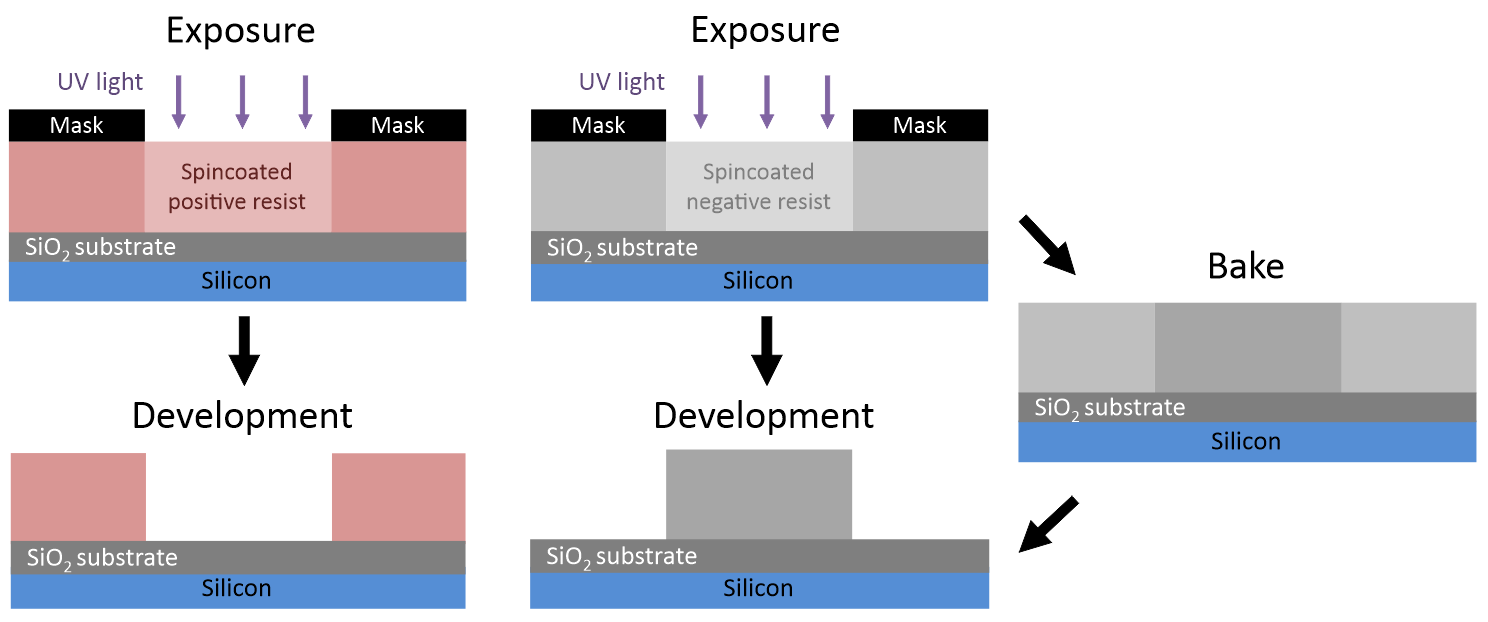
\includegraphics{figures/ch4/positive-negative-photolithography.png}

}

\caption{\label{fig-photolithography-types}A side-view comparison of
generic photolithography processes for positive and negative resists in
the ideal case. Photolithography with a positive resist requires a
single softbake step before exposure, while for negative resists a
second baking step is required after exposure (Thicknesses shown not to
scale).}

\end{figure}

This section details some of the standard photolithography procedures
used in the quarter wafer processing detailed in
Section~\ref{sec-qw-processing}. Photoresists, also referred to here as
``resists'', are UV light-sensitive polymeric resins used for
photolithography. Both positive and negative photoresists were used in
various fabrication processes. Positive resists are made soluble in
alkalines by UV light exposure, meaning exposed areas are removed in the
development process. Conversely, negative resists are cross-linked by
exposure and a post-exposure bake step. The unexposed areas of the
negative resist are then removed in the development process
\autocite{Microchemicals}. Figure~\ref{fig-photolithography-types} gives
a visual representation of these differences.

The specific photoresist selected for photolithography depends on the
specific use case. The types used in this thesis are positive and
negative AZ\(^\circledR\) photoresists (AZ\(^\circledR\) 1518,
Microchemicals GmbH; AZ\(^\circledR\) nLOF 2020, Microchemicals GmbH)
and SU-8 (SU8-2150, Kayaku Advanced Materials, formerly Microchem). The
AZ\(^\circledR\) resists used here have a minimum film thickness of
\(1.5\textrm{ } \mu \textrm{m}\) \autocite{Microchemicals}, while the
SU8-2150 has a minimum film thickness of
\(0.5\textrm{ } \mu \textrm{m}\) \autocite{Kayaku}. Positive resists
which have not been thermally crosslinked will soften at higher
temperatures (\(\gtrsim 100^\circ\)C for AZ\(^\circledR\) 1518), leading
to a rounded profile. This is not the case for negative resists, which
are more thermally stable \autocite{Microchemicals}. Each resist
therefore has a different cross-section profile, as shown in
Figure~\ref{fig-photolithography-profiles}.

\begin{figure}

\begin{minipage}[t]{0.47\linewidth}

{\centering 

\raisebox{-\height}{

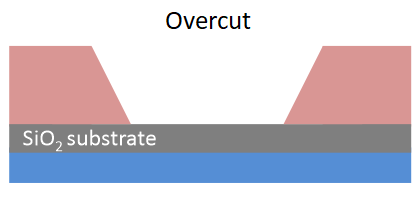
\includegraphics{figures/ch4/overcut-profile.png}

}

}

\subcaption{\label{fig-overcut-profile}}
\end{minipage}%
%
\begin{minipage}[t]{0.05\linewidth}

{\centering 

~

}

\end{minipage}%
%
\begin{minipage}[t]{0.47\linewidth}

{\centering 

\raisebox{-\height}{

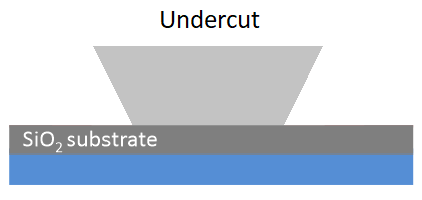
\includegraphics{figures/ch4/undercut-profile.png}

}

}

\subcaption{\label{fig-undercut-profile}}
\end{minipage}%

\caption{\label{fig-photolithography-profiles}The overcut profile of a
positive resist pattern is shown in (a). The undercut profile in (b) is
ideal for thin-film metal deposition and subsequent patterned removal,
known as ``lift-off''. Each profile has had the central region of the
substrate exposed to UV light prior to development.}

\end{figure}

If metal deposition is performed on a positive resist, some metal can
collect on the outwardly-sloped sidewalls of the resist (see
Figure~\ref{fig-photolithography-profiles}) which forms significant
spikes on the edges of the deposited metal upon lift-off. On the other
hand, metal cannot collect on top of the inwardly-sloped negative
profile sidewalls, which avoids the formation of large edge spikes.
Therefore, the negative resist profile is more suited to metal or metal
oxide deposition and lift-off processes, though the process is more
sensitive to human error due to requiring more processing steps than
positive resist \autocite{Microchemicals}. Finally, when it is suitably
processed SU-8 is considered to be more stable and biocompatible than
other photoresists \autocite{Albarghouthi2022}. It is especially
biocompatible when chemically modified via processes such as isopropanol
sonication and O\(_2\) plasma treatment \autocite{Chen2021}.

All photolithographic exposure was performed using a Karl Suss MJB3
Contact Aligner with a USHIO super-high pressure 350 W mercury lamp
(USH-350DS, Japan). When performing photolithography, the intensity
reading from the aligner was \(20.8-24.2\) mW/cm\(^2\) (Note however
that an external photometer reading at 400 nm found an intensity output
of 17.2 mW/cm\(^2\) when the aligner read 21.0 mW/cm\(^2\)).

In general, photolithography procedures should be performed under yellow
lighting, as light wavelengths from \(320-450\) nm can promote reactions
in the photoresist used. Aging of photoresist over time can also
significantly affect the photolithography process, and therefore all
processes should be re-optimised regularly over time to give the desired
result \autocite{Microchemicals}. The range in processing times for some
steps of the processes used here are largely due to the effects of aging
on the photoresist.

The step-by-step processes for each resist are detailed in the
subsequent sections.

\hypertarget{azcircledr-1518-photoresist}{%
\subsection{\texorpdfstring{AZ\(^\circledR\) 1518
photoresist}{AZ\^{}\textbackslash circledR 1518 photoresist}}\label{azcircledr-1518-photoresist}}

\begin{enumerate}
\def\labelenumi{\arabic{enumi}.}
\item
  Spincoat at a final speed of 4000 rotations per minute (rpm) for 1
  minute, with an initial acceleration of 500 rpm/s (notes: clean the
  substrate with acetone, isopropanol (IPA) and nitrogen before
  spincoating; use only the minimum amount of photoresist required to
  fully cover the wafer surface; avoid any gaps or bubbles in the
  photoresist).
\item
  Softbake \(2-4\) minutes at \(95^\circ\)C on the hotplate (2 min for
  individual devices, 4 min for a quarter wafer)
\item
  Mask expose for \(10-12\) s (note: clean mask with acetone/IPA and
  N\(_2\) dry before use)
\item
  Develop with 3 parts AZ\(^\circledR\) 326 (2.38 \% TMAH metal-ion free
  developer, Microchemicals GmbH) in 1 part deionised (DI) water for
  \(30-45\) s (note: rinse for \(10-15\) s in one development solution,
  then perform the rest of the development in clean developer for a
  cleaner profile; lightly agitate the solution throughout the
  development process)
\item
  Rinse device for 30 s in DI water to remove excess developer, then dry
  under nitrogen
\end{enumerate}

\hypertarget{azcircledr-nlof-2020-photoresist}{%
\subsection{\texorpdfstring{AZ\(^\circledR\) nLOF 2020
photoresist}{AZ\^{}\textbackslash circledR nLOF 2020 photoresist}}\label{azcircledr-nlof-2020-photoresist}}

\begin{enumerate}
\def\labelenumi{\arabic{enumi}.}
\item
  Spincoat at final speed of 3000 rotations per minute (rpm) for 1
  minute, with an initial acceleration of 500 rpm/s (notes: clean the
  substrate with acetone, isopropanol (IPA) and nitrogen before
  spincoating; avoid any gaps or bubbles in the photoresist)
\item
  Softbake for precisely 60 s at \(110^\circ\)C on the hotplate
\item
  Mask expose for \(2.7-3\) s (note: clean mask with acetone/IPA and
  N\(_2\) dry before use)
\item
  Post-exposure bake for precisely 60 s at \(110^\circ\)C on the
  hotplate to cross-link exposed resist
\item
  Develop with 3 parts AZ\(^\circledR\) 326 in 1 part DI water for
  \(60-70\) s (note: rinse for 30 s in one development solution, then
  perform the rest of the development in clean developer for a cleaner
  profile; lightly agitate the solution throughout the development
  process)
\item
  Rinse device for 30 s in DI water to remove excess developer, then dry
  under nitrogen
\end{enumerate}

\hypertarget{su8-2150-photoresist}{%
\subsection{SU8-2150 photoresist}\label{su8-2150-photoresist}}

\begin{enumerate}
\def\labelenumi{\arabic{enumi}.}
\item
  SU-8 was diluted in cyclopentanone until viscosity was low enough to
  spincoat on substrate and then sonicated at \(50^\circ\)C for \(3-4\)
  hours (Note: The dilution ratio used was \textasciitilde1 part SU-8 to
  5 parts cyclopentanone. However, the age of the SU-8 may mean that
  significant evaporation had occurred prior to use, and the amount of
  SU-8 actually present is underrepresented by this ratio)
\item
  Spincoat first with a final speed of 500 rpm (acceleration 500 rpm/s)
  for 10 seconds, followed by spincoating at 4000 rpm (acceleration 7500
  rpm/s) for 40 s.
\item
  Softbake for 10 minutes at \(95^\circ\)C on the hotplate
\item
  Mask expose for \(6-8\) s (note: clean mask with acetone/IPA and
  N\(_2\) dry before use)
\item
  Post-exposure bake for 10 minutes at \(95^\circ\)C on the hotplate to
  cross-link exposed resist
\item
  Develop with SU-8 developer (Kayaku Advanced Materials, formerly
  Microchem) for \(10-15\) s, then clean in IPA for 30 s, repeat this
  step once then dry under nitrogen (note: lightly agitate the solution
  throughout the development process)
\end{enumerate}

\hypertarget{sec-qw-processing}{%
\section{Fabrication of Carbon Nanotube and Graphene Field-Effect
Transistors}\label{sec-qw-processing}}

\hypertarget{general-remarks}{%
\subsection{General Remarks}\label{general-remarks}}

\begin{figure}

{\centering 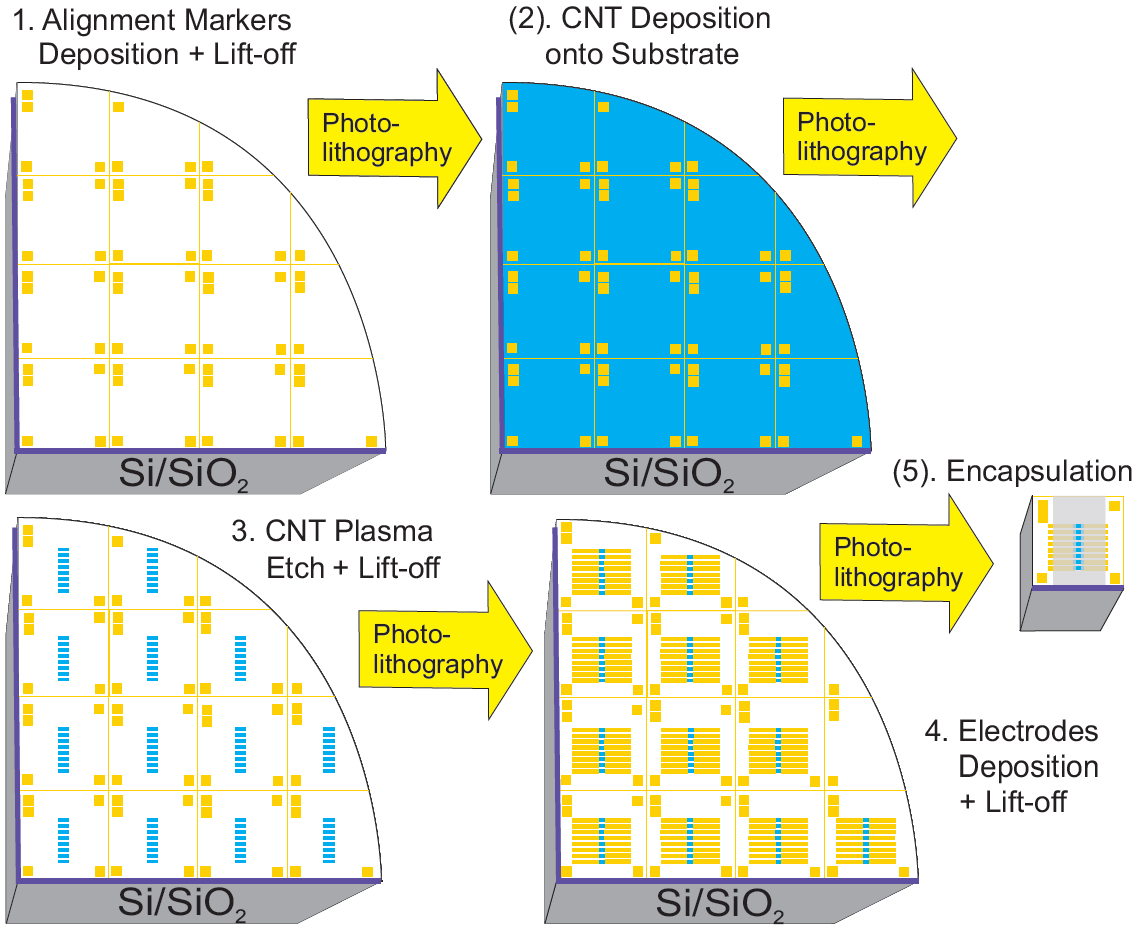
\includegraphics[width=0.9\textwidth,height=\textheight]{figures/ch4/photolithography-cycle.png}

}

\caption{\label{fig-qw-photolithography}The photolithographic processes
used for fabrication of both carbon nanotube and graphene devices
(graphene devices were fabricated individually for every step. Step \#2
is passed over for graphene devices).}

\end{figure}

Photolithography was used to define eight channel regions on each device
and subsequently to define metal contacts for each of these channels. A
schematic demonstrating these photolithography processes on a quarter
wafer is shown in Figure~\ref{fig-qw-photolithography}. Masks for
photolithography were designed in-house using LayoutEditor CAD software
and patterned externally with a UV laser writer.

Thermal evaporation was used when depositing chromium (Cr-plated
tungsten rods, Kurt J. Lesker) and gold (Au wire, 99.99\%, Regal
Castings Ltd.), while electron beam evaporation was used when depositing
titanium (Ti pieces, 99.99\%, Kurt J. Lesker) and metal oxides
(\emph{e.g.} Al\(_2\)O\(_3\) pieces, 99.99\%, Kurt J. Lesker). Metal and
metal oxide deposition was performed using an Angstrom Engineering
Nexdep 200 Vacuum Deposition System. Deposition thickness was monitored
by a Inficon quartz piezoelectric sensor and controlled using an Inficon
Deposition Controller. Electron beam power was provided by a Telemark
TT-6 power supply. For metals, the chamber was initially evacuated to a
pressure \(5 \times 10^{-6}\) mTorr, while for metal oxides the chamber
was initially evacuated to a pressure of \(1 \times 10^{-5}\) mTorr.
After evaporation, the chamber was cooled and vented with nitrogen.

Carbon nanotube network field-effect transistors were fabricated using
4-inch \(p\)-type (B-doped) silicon wafers with either a 100 nm or 300
nm SiO\(_2\) layer (WaferPro LLC) as the substrate. Devices intended for
backgated measurements were fabricated with a 100 nm SiO\(_2\) layer.
Before photolithographic processing, the wafers were spin-coated with
AZ\(^\circledR\) 1518 photoresist, placed photoresist-side down onto a
cleanroom wipe, fixed in place using vacuum suction, then cleaved into
quarters using a diamond-tipped scribe tool. For fabrication performed
before June 2023, the protective photoresist layer was then removed by
soaking the quarter-wafers in acetone for 15 minutes, then rinsed with
isopropyl alcohol (IPA) and dried with N\(_2\) gas. However, for
complete removal of photoresist, we found it was necessary to flood
expose the wafer with the Karl Suss Aligner for 1 min and then place it
in AZ\(^\circledR\) 326 developer for 3 min, as discussed further in
\textbf{?@sec-photoresist-contamination}.

Graphene field-effect transistors were fabricated using 300 nm
SiO\(_2\)/p-type Si substrates covered with a monolayer of mechanically
transferred CVD graphene (Advanced Chemical Supplier). This substrate
was cleaved into equal-sized square chips before photolithography, with
side length between \(11.6-11.7\) mm, subject to variability in wafer
size. The same cleaving process outlined in
Section~\ref{sec-dep-carbon-nanotubes} was used for cleaving the chips,
but the photoresist was not rinsed off after cleaving. Devices were
exposed to a brief burst of N\(_2\) gas to remove any dust from the
cleaving process from the surface of devices. When not being used in
photolithography, graphene-based devices were stored in a vacuum
desiccator to prevent the quality of the graphene deteriorating with
exposure to air over time. The limited adhesion of graphene to the wafer
meant that photolithographic processing had to be performed particularly
carefully when fabricating graphene devices.

From Jul 2023 onwards, after each photolithography step using negative
resist, quarter wafers/chips were placed in AZ\(^\circledR\) 326 or SU8
developer (depending on the type of resist) for 3 min to ensure complete
removal of photoresist residue. For each step with positive resist, the
same procedure was performed but with a flood exposure with UV light for
1 min before being placed in developer. The exception to this rule was
for devices with an aluminium oxide layer present. Tetramethylammonium
hydroxide (TMAH), the active ingredient of AZ\(^\circledR\) 326, etches
through aluminium oxide and causes electrical shorts through the
dielectric layer \autocite{Oh2011,Ali2021}. A further discussion showing
the results of this process is given in
\textbf{?@sec-photoresist-contamination}.

\begin{figure}

\begin{minipage}[t]{0.47\linewidth}

{\centering 

\raisebox{-\height}{

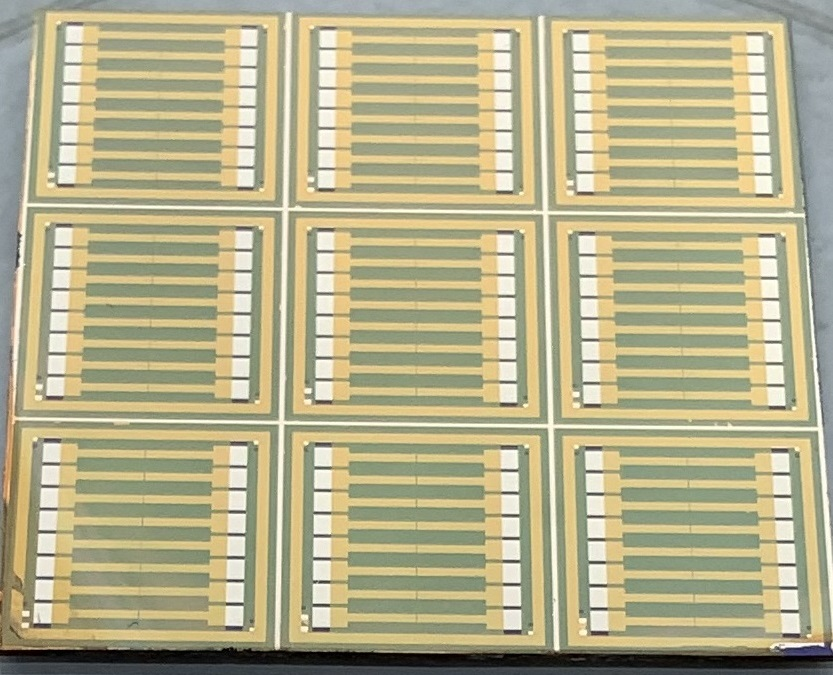
\includegraphics{figures/ch4/IMG_0845.jpg}

}

}

\subcaption{\label{fig-qw-device-photo}}
\end{minipage}%
%
\begin{minipage}[t]{0.05\linewidth}

{\centering 

~

}

\end{minipage}%
%
\begin{minipage}[t]{0.47\linewidth}

{\centering 

}

\end{minipage}%
\newline
\begin{minipage}[t]{0.47\linewidth}

{\centering 

\raisebox{-\height}{

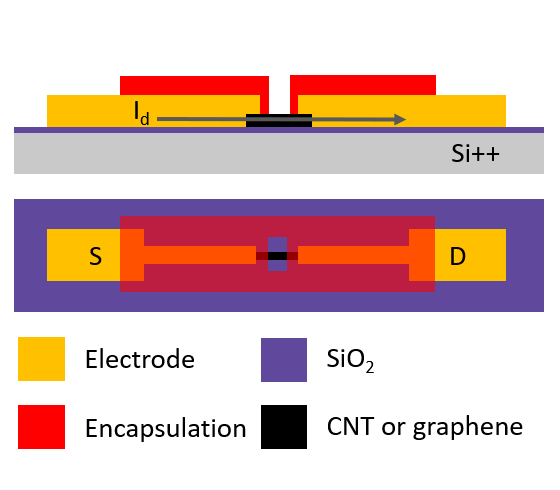
\includegraphics{figures/ch4/fet-schematic.png}

}

}

\subcaption{\label{fig-device-schematic}}
\end{minipage}%
%
\begin{minipage}[t]{0.05\linewidth}

{\centering 

~

}

\end{minipage}%

\caption{\label{fig-field-effect-transistor}A finished quarter-wafer
with the unusable edges cleaved off is shown in (a). Note the double
alignment markers feature in the bottom left corner of each device in
(a), indicating channel 1 `CH1'. The component parts of the field-effect
transistor are labelled on device cross-section and channel top view
schematics in (b).}

\end{figure}

Figure~\ref{fig-qw-device-photo} shows a completed quarter-wafer of
carbon nanotube field-effect transistors, where partial (unusable)
devices at the edges of the wafer have been cleaved off so that only a
square of nine devices remains. An individual FET device after the
completed fabrication process is shown in
\textbf{?@fig-single-device-photo}, and
Figure~\ref{fig-device-schematic} shows cross-section and top view
schematics of the completed device with the component parts labelled.

\hypertarget{sec-align}{%
\subsection{Alignment Markers}\label{sec-align}}

Metal alignment markers were deposited in order to accurately align the
device channels with device electrodes in subsequent photolithography
steps. These alignment markers were asymmetric to indicate the
orientation of the device for subsequent photolithography steps and
electrical characterisation. In later discussion, channel 1 is defined
as the channel placed closest to the large double square alignment
marker feature. For carbon nanotube quarter wafers, alignment markers
were deposited either directly before or after carbon nanotube
deposition (see Section~\ref{sec-dep-carbon-nanotubes} for discussion).
For graphene devices, alignment markers were deposited directly after
cleaving using the protective photoresist layer spincoated prior to
cleaving. AZ\(^\circledR\) 1518 was used for alignment marker
photolithography.

For carbon nanotube devices made before Jun 2022, chromium was used as
an adhesive layer for gold, while for all graphene devices and carbon
nanotube devices made after Jun 2022, titanium was used as the adhesive
layer. Metal layer thickness values quoted here are as stated on the
Inficon controller. Without first corroborating these measurements with
the Dektat profiler, these values should be treated as being strictly
nominal. For chromium/gold depositions, 10 nm of chromium was deposited
followed by a 100 nm Au layer. For titanium/gold depositions, a
\(10-20\) nm of titanium was deposited followed by a 50 nm Au layer.
Devices were then soaked in acetone for at least 2 hours for photoresist
lift-off, washed in IPA and dried with nitrogen. The use of titanium
gave rise to a cleaner lift-off and improved gold adhesion. Using a
relatively thin gold layer (50 nm nominal instead of 100 nm) proved to
still be clearly visible but to a cleaner lift-off. Profiler
measurements of combined metal layer thicknesses after lift-off are
described in Section~\ref{sec-electrodes}.

\hypertarget{sec-dep-carbon-nanotubes}{%
\subsection{Deposition of Carbon
Nanotubes}\label{sec-dep-carbon-nanotubes}}

Carbon nanotubes were deposited before the alignment markers
photolithography step on all wafers fabricated between Aug \(2021-\)Feb
2023, while devices fabricated before Aug 2021 and after Feb 2023 had
the alignment markers photolithography step performed before the
deposition of carbon nanotubes. The process order was first switched in
Aug 2021 as this order led to faster processing times. However, the
order was switched back in Feb 2023 to minimise the exposure of carbon
nanotubes to photolithographic chemical processes.

\hypertarget{solvent-based}{%
\subsubsection*{Solvent-Based}\label{solvent-based}}
\addcontentsline{toc}{subsubsection}{Solvent-Based}

The solvent-based deposition process for the carbon nanotube network in
the second fabrication protocol is as follows. 10 mg of
2-mercaptopyridine (99\%, Sigma-Aldrich) was dissolved in 1 ml ethanol
by sonication until clear. Quarter wafers were sonicated in acetone for
3 min, then exposed to O\(_2\) plasma at 100 W for at least 2 min in a
small plasma cleaner (Plasma Etch, Inc., PE-50 Compact Benchtop Plasma
Cleaning System) or reactive ion etcher (Oxford Instruments,
Plasmalab\(^\circledR\) 80 Plus) under 300 mTorr pressure. The cleaned
SiO\(_2\)/Si surface was then coated with 2-mercaptopyridine for 10
minutes, rinsed with ethanol to remove residual \(2\)-mercaptopyridine,
and then nitrogen dried.

Meanwhile, 5 \(\mu\)g of 99\% semiconducting carbon nanotube bucky paper
(NanoIntegris, IsoNanotubes S-99) was dispersed in 10 mL of anhydrous
1,2-dichlorobenzene (DCB, Sigma Aldrich) by ultrasonication until no
particles were visible to the naked eye. During this time, the
ultrasonic bath temperature was kept between \(20-30^\circ\)C or the
buckypaper would not disperse successfully. The substrates were then
placed into a dish with CNT-DCB suspension and left covered for 1 hour,
dipped into ethanol for 10 min to remove residual solvent and any
unattached carbon nanotube bundles, and then dried with nitrogen.
Devices fabricated using films deposited in this manner are sometimes
referred to here as ``solvent-deposited'' networks.

\hypertarget{surfactant-based}{%
\subsubsection*{Surfactant-Based}\label{surfactant-based}}
\addcontentsline{toc}{subsubsection}{Surfactant-Based}

Two different approaches were used to attach the surfactant-dispersed
carbon nanotubes (CNTs) to the substrate surface. The first approach was
a simple drop-casting method, while the second was performed in the
presence of steam (`steam-assisted'). In both approaches, the quarter
wafers were first rinsed with ultrapure deionised water (DI water),
acetone and IPA. Next, they were placed into a small plasma cleaner
(Plasma Etch, Inc, PE-50 Compact Benchtop Plasma Cleaning System) or
reactive ion etcher (Oxford Instruments, Plasmalab 80 Plus) and exposed
to O\(_2\) plasma at 100 W for at least 2 min under 300 mTorr pressure
to make the surface hydrophilic. 1 mL of poly-L-lysine (PLL) was
immediately deposited onto each quarter wafer and left for 5 minutes.
The quarter wafers were then rinsed for 30 s with DI water and dried
with N\(_2\) gas. The presence of the PLL on the plasma cleaned surface
strengthens the surface adhesion of semiconducting single carbon
nanotubes after the surfactant dispersion has been dropcast onto the
substrate.

For carbon nanotube network films deposited in surfactant without steam
present, 2 mL of IsoNanotubes-S 90\% or 99\% dispersion (NanoIntegris)
was decanted into a small bottle and sonicated for 5 s to break up
bundles of CNTs. (Note: The composition of the surfactant used in the
dispersion is proprietary to NanoIntegris.) An even spread of 400
\(\mu\)L carbon nanotube dispersion was placed in the centre of the
PLL-functionalised quarter wafer, covered with a glass dish and left for
10 minutes. The dispersion was then rinsed off with DI water and IPA,
and the quarter wafer was dried with N\(_2\) gas. Next, the quarter
wafer was annealed in a vacuum oven at 150\(^\circ\) C for 1 hour to
remove residual surfactant. This method would often lead to an
inhomogeneous spread of CNTs across the quarter wafer surface, detailed
further in section \textbf{?@sec-cnt-deposition-effects}.

\begin{figure}

\begin{minipage}[t]{0.47\linewidth}

{\centering 

\raisebox{-\height}{

\includegraphics{figures/ch4/steaming-method-top.png}

}

}

\subcaption{\label{fig-steaming-method-top}}
\end{minipage}%
%
\begin{minipage}[t]{0.05\linewidth}

{\centering 

~

}

\end{minipage}%
%
\begin{minipage}[t]{0.47\linewidth}

{\centering 

\raisebox{-\height}{

\includegraphics{figures/ch4/steaming-method-side.png}

}

}

\subcaption{\label{fig-steaming-method-side}}
\end{minipage}%

\caption{\label{fig-steaming-method}Top view (a) and side view (b) of
the steam-assisted method setup, with and without the glass steam cover
above the quarter wafer.}

\end{figure}

For carbon nanotube network films deposited in surfactant in the
presence of steam, 2 mL of IsoNanotubes-S 90\% or 99\% dispersion
(NanoIntegris) was decanted into a small bottle and burst-sonicated once
(on then off again) to break up bundles of carbon nanotubes. 75 mL of
95\(^\circ\) C water was then placed into a glass dish on a hotplate
held at 95\(^\circ\) C. After this, the PLL-functionalised quarter wafer
was placed in the centre of an insulating surface on the same hotplate.
The carbon nanotube dispersion was carefully spread across the surface
of the wafer without spilling any over the wafer edges. The wafer on the
insulating surface and glass dish were then left under the same glass
dish for 2 minutes to expose the wafer to steam from the glass dish. The
use of an insulating surface meant that the wafer and dispersion were
not heated from below while exposed to steam. The steam-assisted
deposition setup is shown in Figure~\ref{fig-steaming-method}.

The carbon nanotube dispersion was then rinsed off the wafer with DI
water, ethanol, acetone and IPA, and then the quarter wafer was dried
with N\(_2\) gas. As in the original method, the quarter wafer was then
annealed in a vacuum oven at 150\(^\circ\) C for 1 hour to remove
residual surfactant. This method gave an even spread of CNTs across the
quarter wafer surface, leading to a greater consistency in performance
between devices. Further details can be found in
\textbf{?@sec-cnt-deposition-effects}. Devices fabricated using films
deposited in this manner are sometimes referred to here as
``steam-deposited'' or ``steam-assisted surfactant-deposited'' networks
(rather than simply ``surfactant-deposited'', to avoid confusion with
the steam-free method).

\hypertarget{channel-etching}{%
\subsection{Channel Etching}\label{channel-etching}}

\begin{figure}

\begin{minipage}[t]{0.47\linewidth}

{\centering 

\raisebox{-\height}{

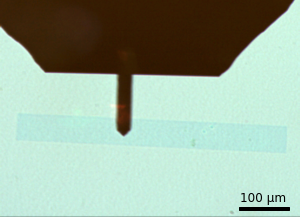
\includegraphics{figures/ch4/channel-area.png}

}

}

\subcaption{\label{fig-graphene-channel-etch}}
\end{minipage}%
%
\begin{minipage}[t]{0.05\linewidth}

{\centering 

~

}

\end{minipage}%
%
\begin{minipage}[t]{0.47\linewidth}

{\centering 

\raisebox{-\height}{

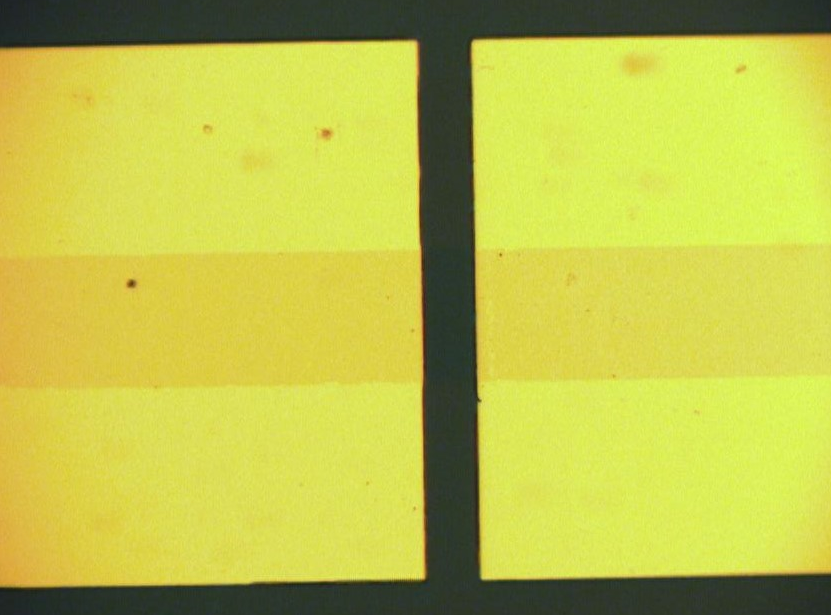
\includegraphics{figures/ch4/graphene-channel-electrodes.png}

}

}

\subcaption{\label{fig-graphene-channel-electrodes}}
\end{minipage}%

\caption{\label{fig-microscope-graphene-channel}A graphene channel after
the plasma etch step is shown in (a), and (b) shows another graphene
channel after the metal electrode deposition and liftoff step.}

\end{figure}

Eight channel features, each 1000 \(\mu\)m in length and 100 \(\mu\)m in
width with a pitch of 1200 \(\mu\)m, were patterned using
AZ\(^\circledR\) 1518 photolithography on each carbon nanotube or
graphene-covered substrate. Unwanted nanomaterial not covered with
photoresist was then etched away with 200 W oxygen plasma at 600 mTorr
using a reactive ion etcher or RIE (Plasmalab\(^\circledR\) 80 Plus,
Oxford Instruments). The etch time was 3 minutes for carbon nanotube
quarter wafers, and 1 minute for graphene chips. The protective
photoresist was then removed by soaking in acetone for at least 5
minutes.

\hypertarget{sec-electrodes}{%
\subsection{Source and Drain Electrodes}\label{sec-electrodes}}

\begin{figure}

\begin{minipage}[t]{0.47\linewidth}

{\centering 

\raisebox{-\height}{

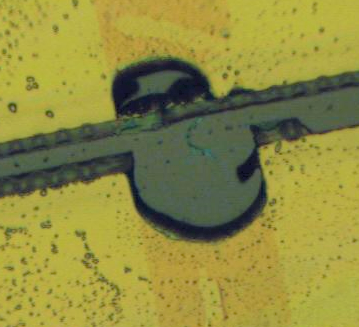
\includegraphics{figures/ch4/apr-21-dmso-damage.png}

}

}

\subcaption{\label{fig-electrode-dmso-damage}}
\end{minipage}%
%
\begin{minipage}[t]{0.05\linewidth}

{\centering 

~

}

\end{minipage}%
%
\begin{minipage}[t]{0.47\linewidth}

{\centering 

\raisebox{-\height}{

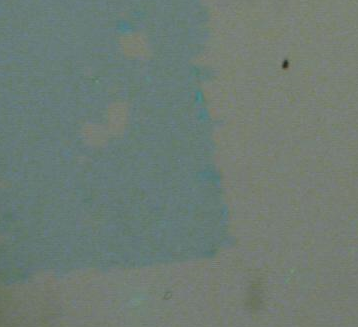
\includegraphics{figures/ch4/may-21-dmso-damage.png}

}

}

\subcaption{\label{fig-graphene-dmso-damage}}
\end{minipage}%

\caption{\label{fig-dmso-damage}Damage to the gold electrode in the
graphene channel region after dimethyl sulfoxide lift-off is shown in
(a), while (b) shows damage to a graphene film (blue-green region) after
dimethyl sulfoxide lift-off.}

\end{figure}

\begin{figure}

\begin{minipage}[t]{0.47\linewidth}

{\centering 

\raisebox{-\height}{

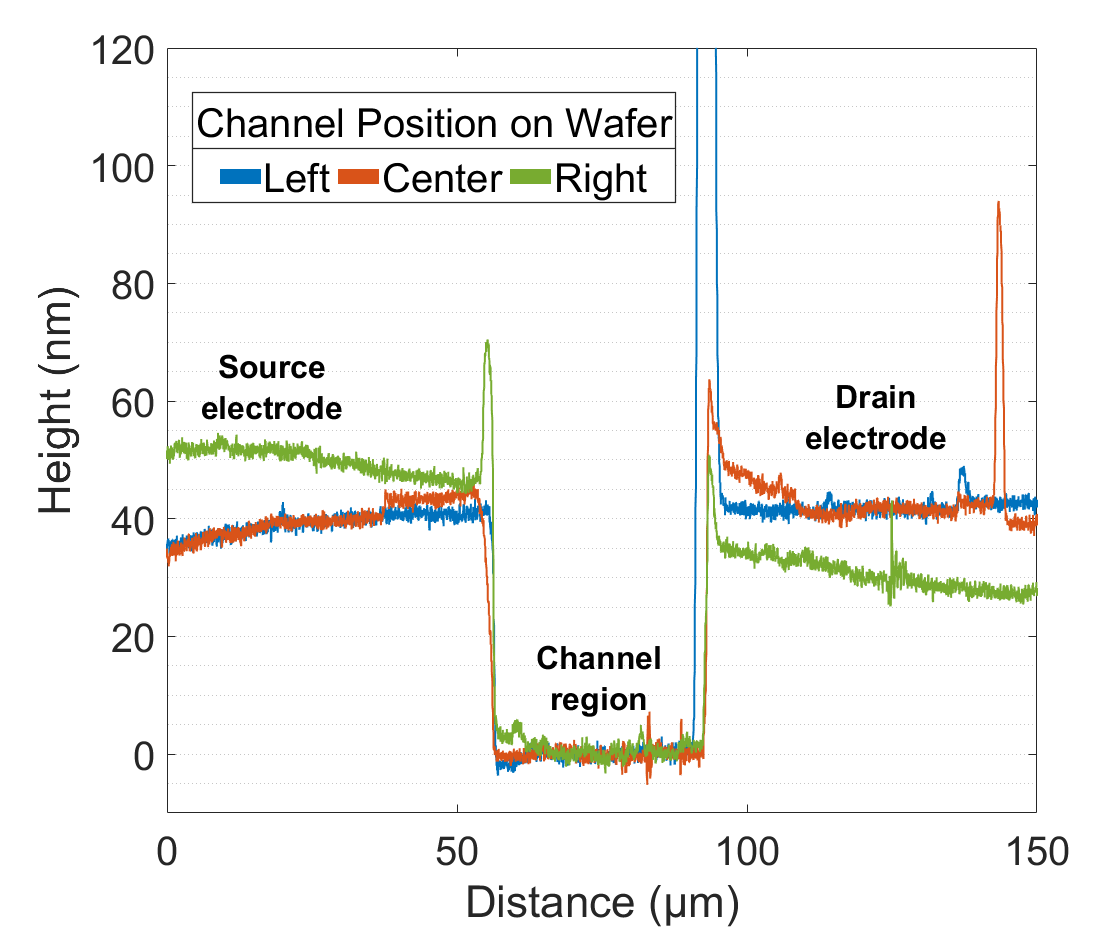
\includegraphics{figures/ch4/dektat_cr_electrodes.png}

}

}

\subcaption{\label{fig-dektat-cr}}
\end{minipage}%
%
\begin{minipage}[t]{0.05\linewidth}

{\centering 

~

}

\end{minipage}%
%
\begin{minipage}[t]{0.47\linewidth}

{\centering 

\raisebox{-\height}{

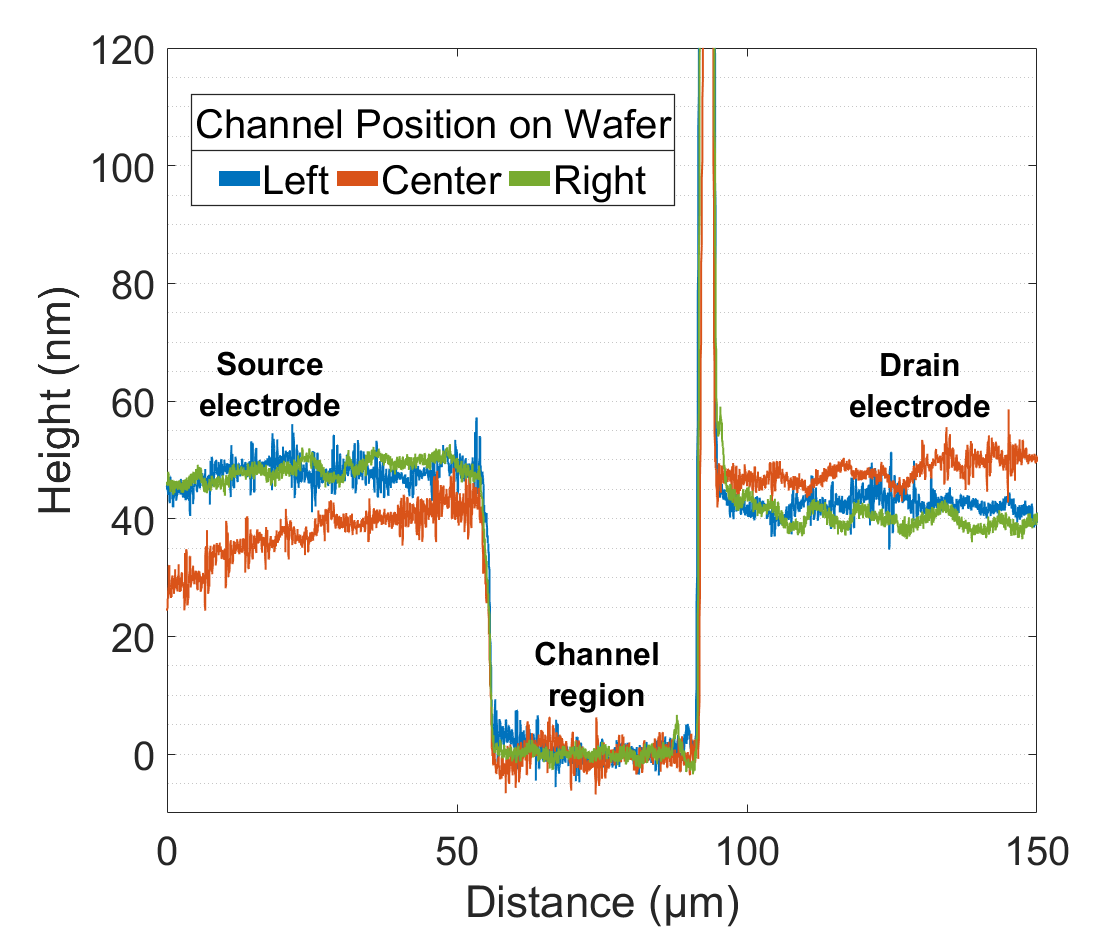
\includegraphics{figures/ch4/dektat_ti_electrodes.png}

}

}

\subcaption{\label{fig-dektat-ti}}
\end{minipage}%
\newline
\begin{minipage}[t]{0.47\linewidth}

{\centering 

\raisebox{-\height}{

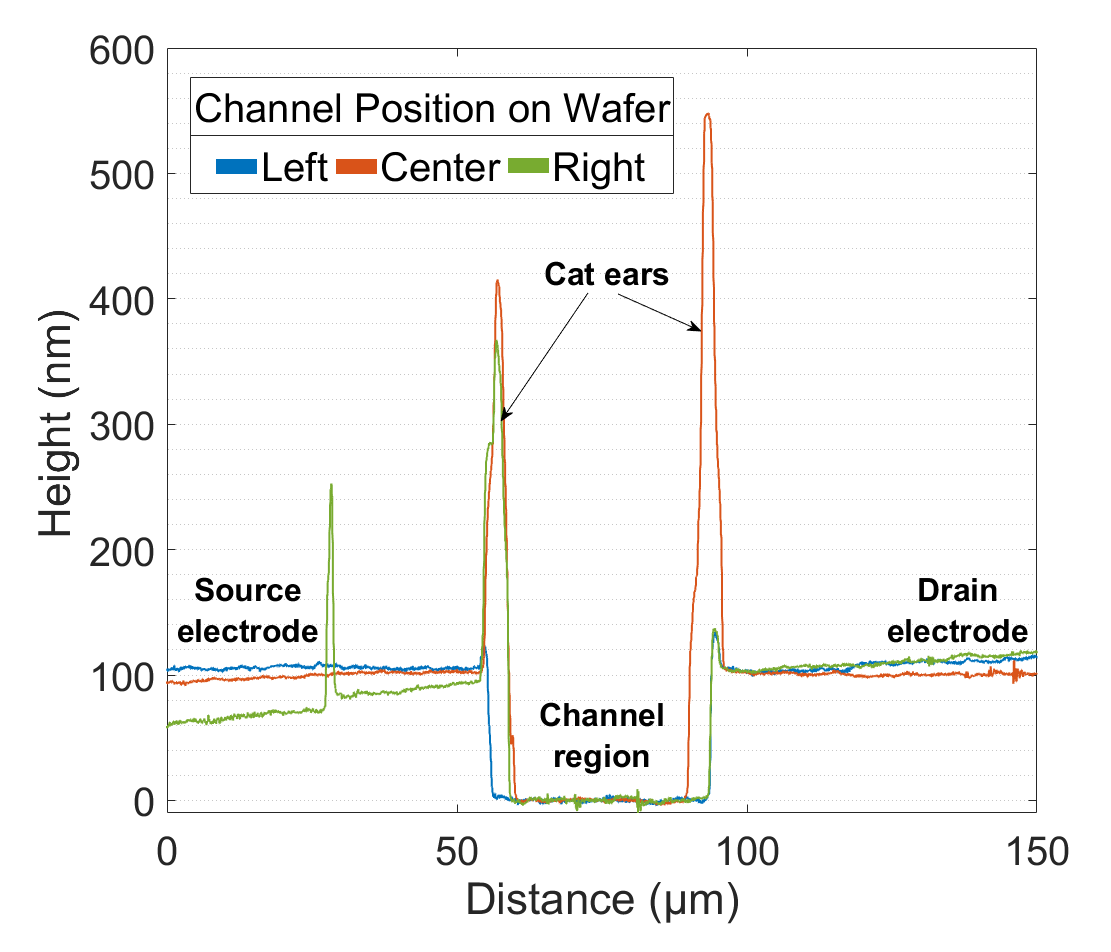
\includegraphics{figures/ch4/dektat_1518_electrode_profile.png}

}

}

\subcaption{\label{fig-dektat-AZ1518-electrode}}
\end{minipage}%
%
\begin{minipage}[t]{0.05\linewidth}

{\centering 

~

}

\end{minipage}%
%
\begin{minipage}[t]{0.47\linewidth}

{\centering 

\raisebox{-\height}{

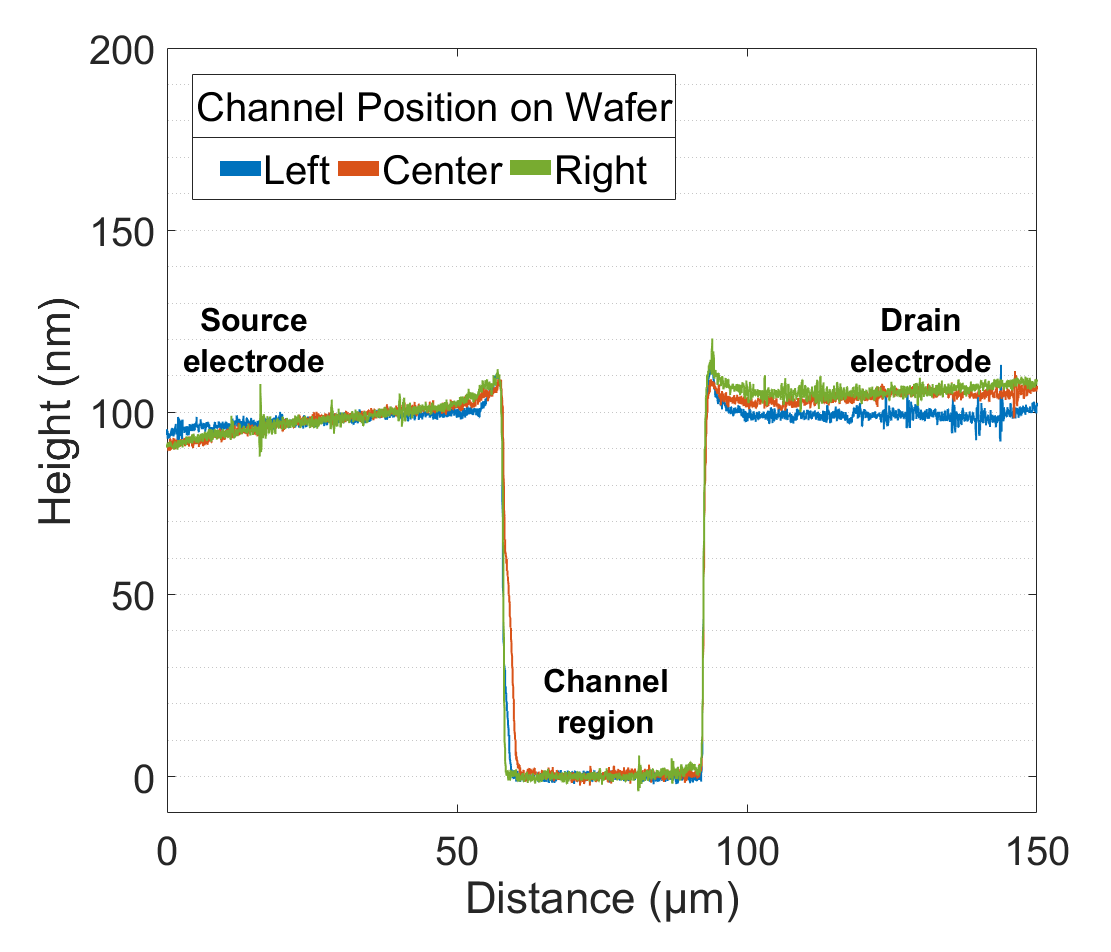
\includegraphics{figures/ch4/dektat_nlof_electrode_profile_2.png}

}

}

\subcaption{\label{fig-dektat-nLOF-electrode}}
\end{minipage}%

\caption{\label{fig-electrodes-dektat}The Dektat height profile
measurements for source and drain electrodes taken at different
locations on four different quarter wafers are shown here. A 10 nm
adhesion layer and 100 nm Au layer were used for the wafers in (a) and
(b), with chromium as the adhesion layer for (a) and titanium for (b). A
20 nm titanium adhesion layer and 100 nm Au layer were used for both (c)
and (d). AZ\(^\circledR\) 1518 photolithography was used for patterning
before metal deposition in (a)-(c), which led to the formation of edge
features or ``cat ears'', with (c) illustrating the full height of these
features. In comparison, (d) shows the profile of electrodes from a
quarter wafer patterned with AZ\(^\circledR\) nLOF2020, where edge
features are greatly reduced.}

\end{figure}

The source and drain electrodes for each channel were patterned using
photolithography with either AZ\(^\circledR\) 1518 photoresist (pre-Mar
2023) or AZ\(^\circledR\) nLOF 2020 photoresist (post-Mar 2023). Before
metal deposition, the developed photoresist pattern was exposed to
O\(_2\) plasma at 50 W for up to 5 s or at 20 W for \(20-25\) s in a
PE-50 plasma cleaner (Plasma Etch, Inc.) to remove residual photoresist
on the developed regions and ensure a clean lift-off. After metal,
wafers/devices were soaked in acetone for at least 2 hours for
photoresist lift-off, washed in IPA and dried with nitrogen.

As with the alignment markers deposition (see Section~\ref{sec-align}),
before Jun 2022 chromium was used for the gold adhesion layer, and after
Jun 2022 titanium was used. Adhesion layers are required to stick metals
such as gold and platinum to silicon dioxide \autocite{Guarnieri2014}. A
20 nm nominal titanium layer instead of 10 nm nominal was found to give
better electrode adhesion, and devices after Feb 2023 were made using
this thicker adhesion layer. Good electronic contact could be made with
electrodes with a nominal gold layer thickness of \(60-100\) nm, and a
Au layer nominally 100 nm thick was most commonly used.

Dimethyl sulfoxide (DMSO) was sometimes used in electrodes lift-off
instead of acetone between Jul 2021 and Feb 2023 because of its
effectiveness as a photoresist stripping agent. However, it was
abandoned due to some indications it was unsuitable for the devices
being fabricated, as shown in Figure~\ref{fig-dmso-damage} and also as
detailed in \textbf{?@sec-cnt-deposition-effects}. It is possible that
heat from the electrodes deposition sometimes crosslinked residual
photoresist on the nanomaterial, and then during lift-off was removed
together with any attached nanomaterial by the DMSO. However, it is also
possible that prolonged exposure to DMSO alone was sufficient to detach
nanomaterial from the substrate. Therefore, acetone was the preferred
agent for lift-off despite being a less efficient stripping agent than
DMSO.

Example height profiles of quarter wafer channels taken using a Veeco
Dektat 150 profiler are shown in Figure~\ref{fig-electrodes-dektat}.
AZ\(^\circledR\) 1518 photoresist was used in Figure~\ref{fig-dektat-cr}
and Figure~\ref{fig-dektat-ti} for photolithographic patterning. A 10 nm
adhesion layer and 100 nm Au layer were used for each quarter wafers to
ensure a consistent comparison. From these figures, we find an measured
Cr/Au electrode height of \(42\pm1\) nm and an measured Ti/Au electrode
height of \(48\pm2\) nm, slightly less than half the respective heights
stated on the Inficon Deposition Controller.

Although using AZ\(^\circledR\) nLOF 2020 photolithography involves more
processing steps, it gave rise to more cleanly-defined electrodes with a
more consistent height profile. Often electrode deposition using
AZ\(^\circledR\) 1518 photoresist would lead to sharp vertical spikes
along the edge of the electrode, as seen in
Figure~\ref{fig-dektat-AZ1518-electrode}. These edge spikes or ``cat
ears'' can partially or fully protrude through thin encapsulation
materials such as SU8 and Al\(_2\)O\(_3\), leading to significant
leakage currents from the electrodes into the FET top gate. This effect
is due to the profile of positive resists being suboptimal for lift-off
processes, as discussed in Section~\ref{sec-photolithography}.

The height profile corresponding to a wafer with electrodes fabricated
using AZ\(^\circledR\) nLOF 2020 is shown in
Figure~\ref{fig-dektat-nLOF-electrode}. A 20 nm titanium adhesion layer
and 100 nm Au layer were used for both
Figure~\ref{fig-dektat-AZ1518-electrode} and
Figure~\ref{fig-dektat-nLOF-electrode} to ensure a consistent
comparison, resulting in a measured electrode height of \(103\pm2\) nm
for both wafers. By comparing these figures, we see AZ\(^\circledR\)
nLOF 2020 photoresist has a more consistent electrode height profile
across the wafer surface than the wafer which used AZ\(^\circledR\) 1518
resist. The measured edge features for the AZ\(^\circledR\) 1518 resist
electrodes vary in size from 20 nm to 450 nm above the bulk electrode
surface, whereas the edge features for the AZ\(^\circledR\) nLOF 2020
resist do not exceed 14 nm in height.

\hypertarget{sec-encapsulation}{%
\subsection{Encapsulation}\label{sec-encapsulation}}

Several different approaches were used for the encapsulation, or contact
protection, of devices. The encapsulation of graphene and
carbon-nanotube transistors for biosensing is essential to improve
transistor characteristics, passivate the electrodes and ensure only the
nanomaterial region is active during biosensing, as discussed in
\textbf{?@sec-biosensor-methods}.

Before encapsulation photolithography the carbon-nanotube network
quarter wafers were cleaved into individual 11 mm \(\times\) 11 mm
chips, using the cleaving process outlined in
Section~\ref{sec-dep-carbon-nanotubes}. Cleaving the devices at this
step simplified mask alignment and ensured consistent thickness across
photoresist encapsulated devices.

Two different photolithography masks were used for encapsulation
photolithography in this work, with different exposed areas of active
nanomaterial. The first mask was used for devices made before Jan 2023,
and was designed to leave a region of 500 \(\mu\)m \(\times\) 10
\(\mu\)m unencapsulated for each channel. The second mask was used
exclusively after Jan 2023, and was designed to leave a region of 200
\(\mu\)m \(\times\) 20 \(\mu\)m unencapsulated for each channel. This
change was made to double the area of carbon nanotubes exposed to
electrolyte while halving the area of SiO\(_2\) dielectric exposed to
electrolyte during aqueous sensing.

\begin{figure}

\begin{minipage}[t]{0.47\linewidth}

{\centering 

\raisebox{-\height}{

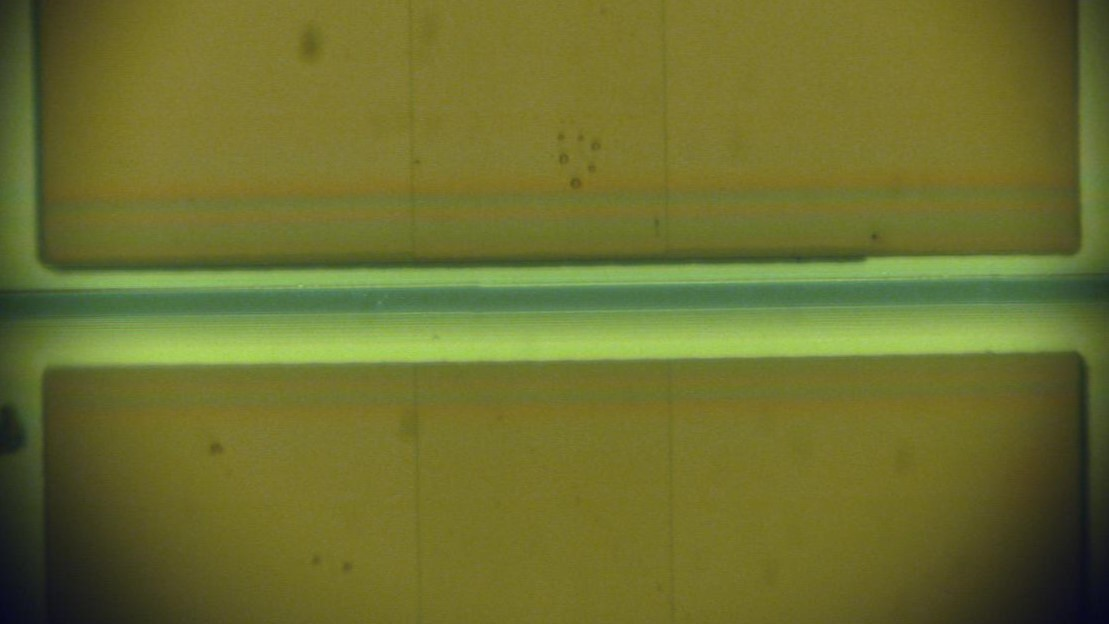
\includegraphics{figures/ch4/encapsulation_old.png}

}

}

\subcaption{\label{fig-encapsulation-old}}
\end{minipage}%
%
\begin{minipage}[t]{0.05\linewidth}

{\centering 

~

}

\end{minipage}%
%
\begin{minipage}[t]{0.47\linewidth}

{\centering 

\raisebox{-\height}{

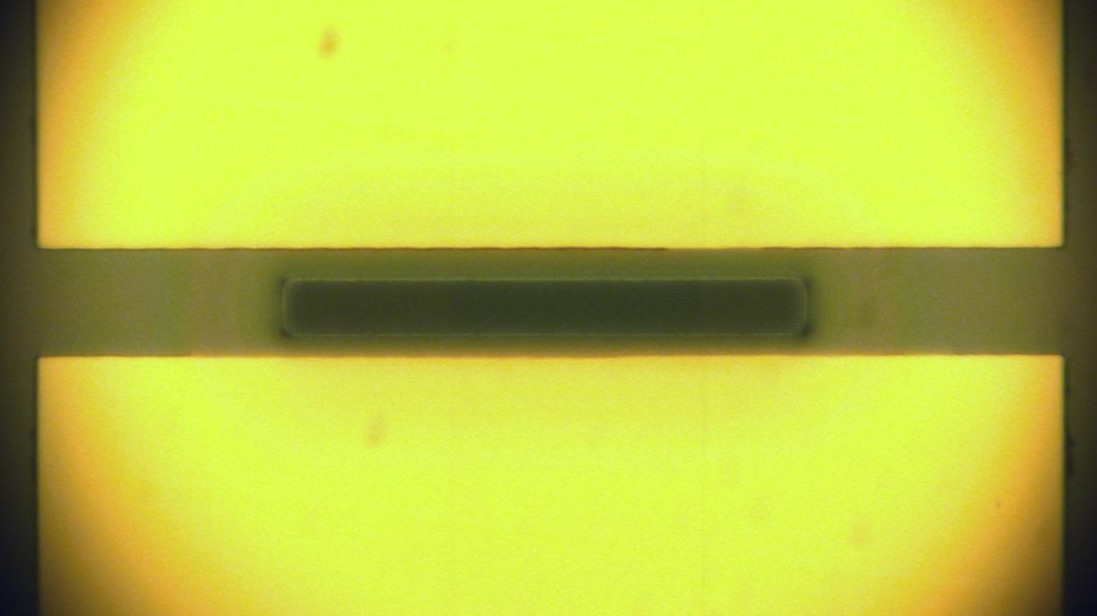
\includegraphics{figures/ch4/encapsulation_new.png}

}

}

\subcaption{\label{fig-encapsulation-new}}
\end{minipage}%

\caption{\label{fig-microscope-encapsulation}Figures showing
encapsulation with hardbaked AZ\(^\circledR\) 1518 using the pre-2023
mask in (a), and the 2023 mask in (b).}

\end{figure}

A side-by-side microscope comparison of hardbaked AZ\(^\circledR\) 1518
processed with each mask is given in
Figure~\ref{fig-microscope-encapsulation}, while a Dektat profile
comparison corresponding to Figure~\ref{fig-microscope-encapsulation} is
shown in \textbf{?@fig-old-new-mask}. The profiles corresponding to the
mask used after Jan 2023 clearly exhibit greater device-to-device
consistency, partly due to the mask requiring a greater level of
accuracy when aligning the encapsulation pattern with the electrode
channel. The larger feature size also means development time has less of
an impact on the quality of the encapsulation opening.

\hypertarget{photoresist-encapsulation}{%
\subsubsection*{Photoresist
encapsulation}\label{photoresist-encapsulation}}
\addcontentsline{toc}{subsubsection}{Photoresist encapsulation}

\begin{figure}

\begin{minipage}[t]{0.47\linewidth}

{\centering 

\raisebox{-\height}{

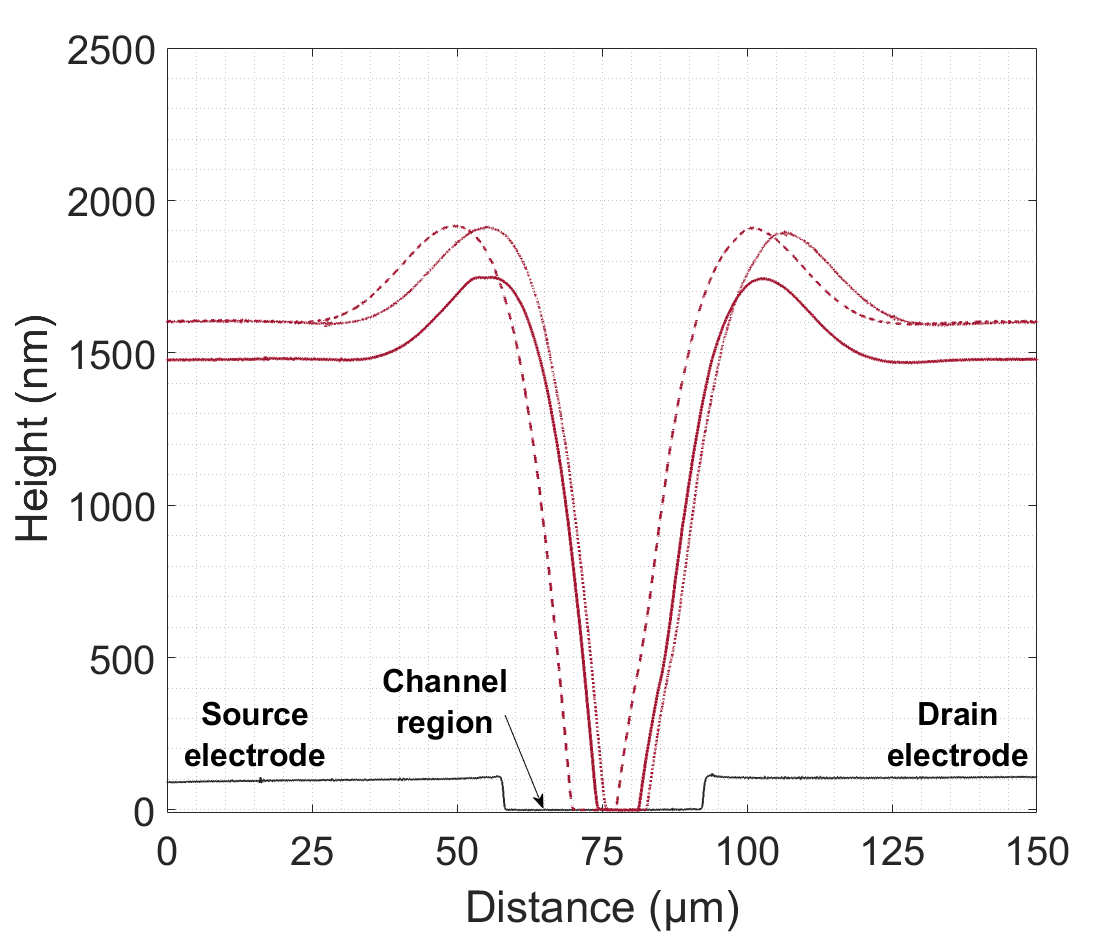
\includegraphics{figures/ch4/dektat_AZ1518_oldmask.png}

}

}

\subcaption{\label{fig-AZ1518-old}}
\end{minipage}%
%
\begin{minipage}[t]{0.05\linewidth}

{\centering 

~

}

\end{minipage}%
%
\begin{minipage}[t]{0.47\linewidth}

{\centering 

\raisebox{-\height}{

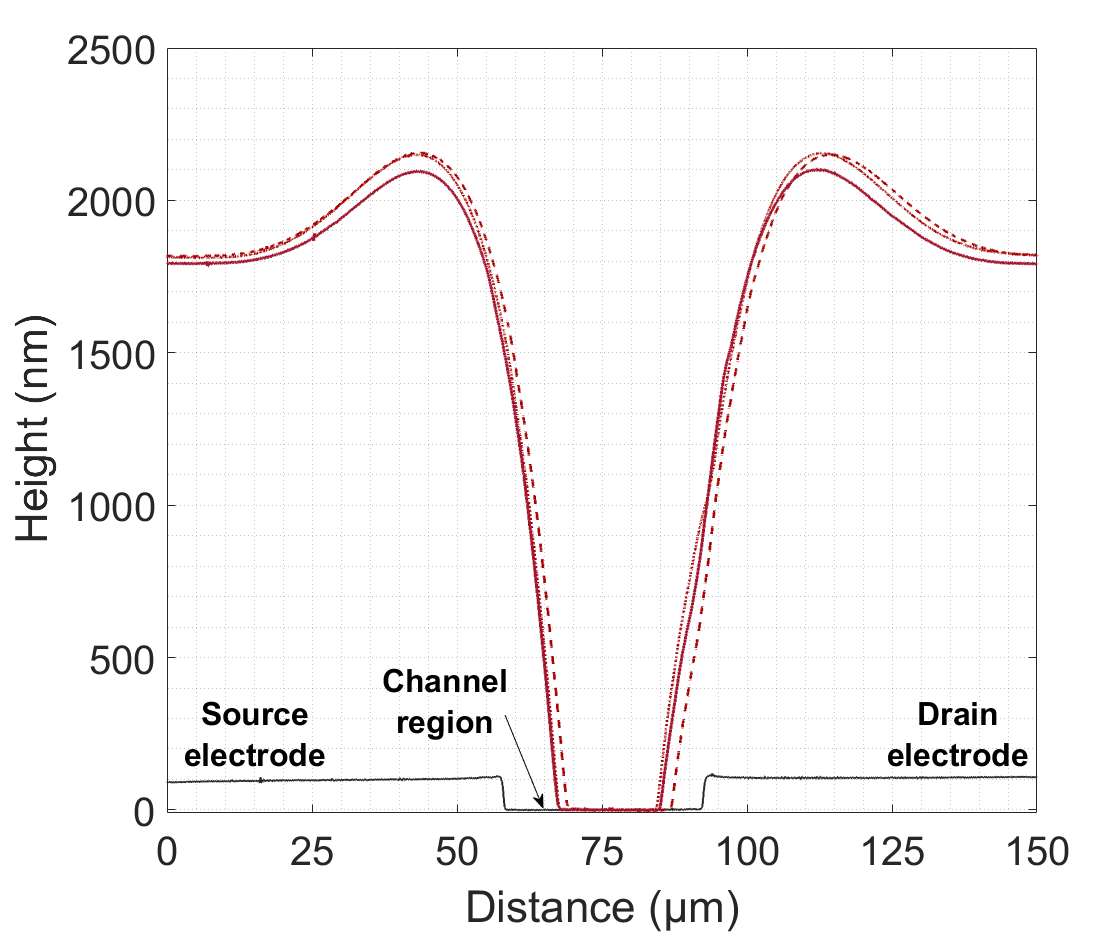
\includegraphics{figures/ch4/dektat_AZ1518_newmask.png}

}

}

\subcaption{\label{fig-AZ1518-new}}
\end{minipage}%
\newline
\begin{minipage}[t]{0.47\linewidth}

{\centering 

\raisebox{-\height}{

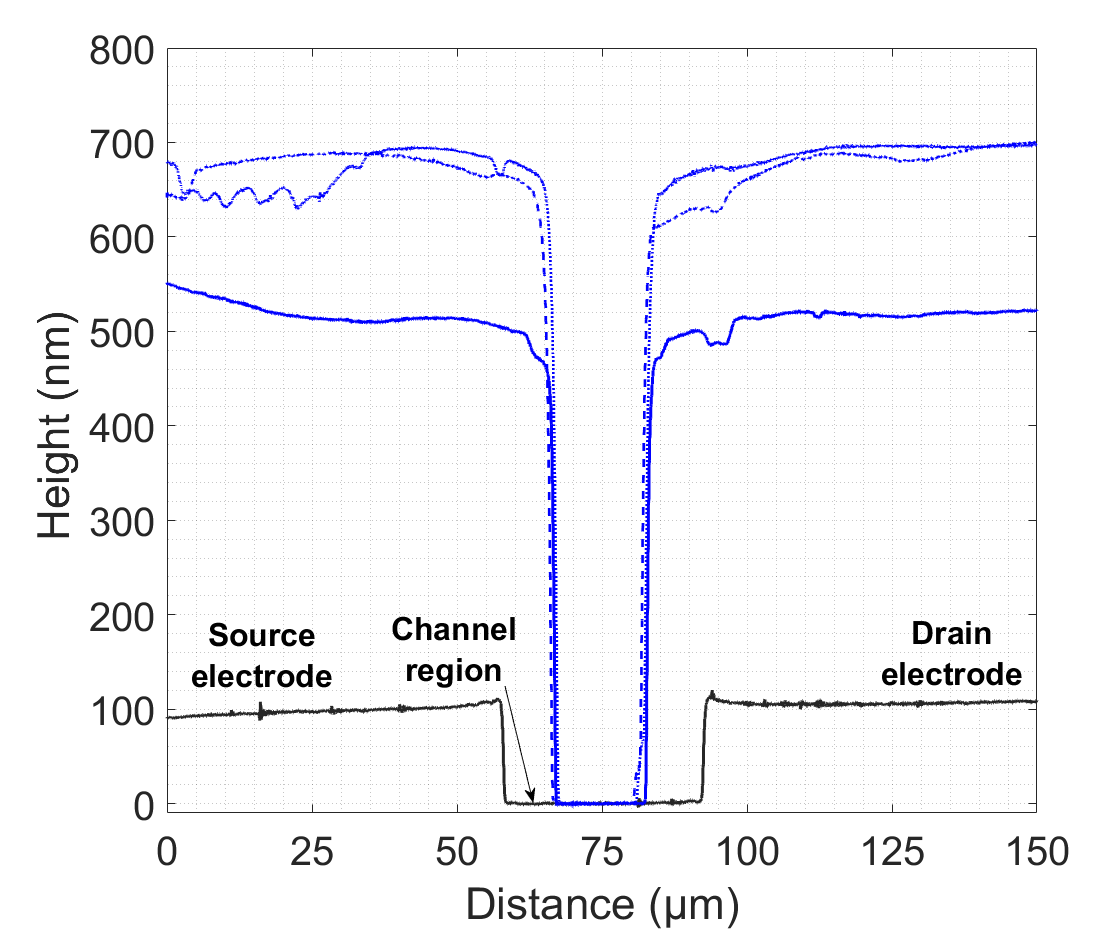
\includegraphics{figures/ch4/dektat_SU8_newmask.png}

}

}

\subcaption{\label{fig-SU8-new}}
\end{minipage}%
%
\begin{minipage}[t]{0.05\linewidth}

{\centering 

~

}

\end{minipage}%
%
\begin{minipage}[t]{0.47\linewidth}

{\centering 

\raisebox{-\height}{

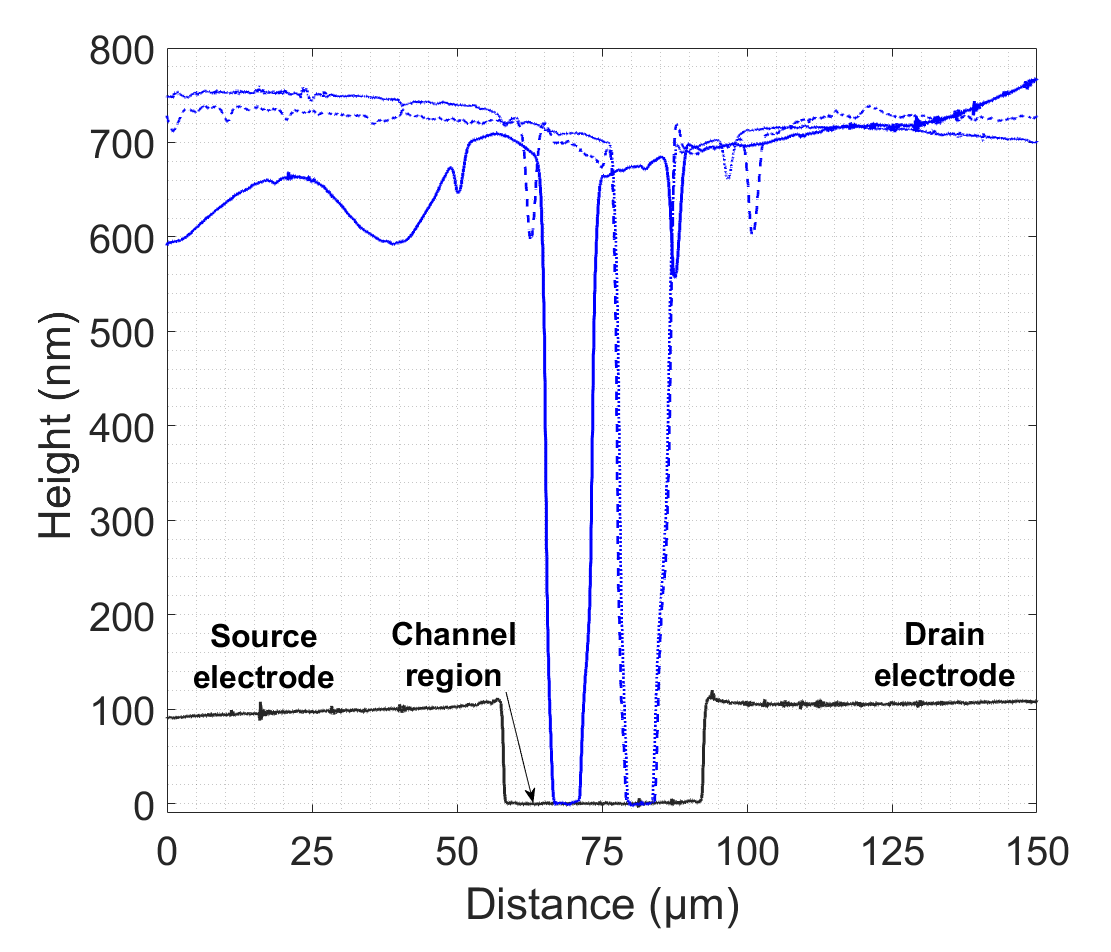
\includegraphics{figures/ch4/dektat_SU8_oldmask.png}

}

}

\subcaption{\label{fig-SU8-old}}
\end{minipage}%

\caption{\label{fig-dektat-encapsulation}Dektat of carbon nanotube
devices after encapsulation photolithography using hardbaked
AZ\(^\circledR\) 1518 and SU-8 2150, taken from various devices. (a) and
(c) show photolithography performed with the old, pre-2023 mask, using
AZ\(^\circledR\) 1518 and SU-8 2150 respectively. (b) and (d) show
photolithography performed with the new mask from 2023 onwards, using
AZ\(^\circledR\) 1518 and SU-8 2150 respectively.}

\end{figure}

Two types of photoresist were initially trialled for encapsulation of
carbon nanotube network devices, AZ\(^\circledR\) 1518 and SU8-2150.
Both AZ\(^\circledR\) 1518
\autocite{Murugathas2018,Murugathas2019b,Shkodra2021} and SU-8 have been
previously used for device encapsulation, with SU-8 noted for being
particularly stable and biocompatible
\autocite{Lee2006,Chen2021,Albarghouthi2022}.

Once developed, the photoresist pattern was exposed to O\(_2\) plasma at
50 W for up to 5 s or at 20 W for \(20-25\) s to remove excess
photoresist from the encapsulation opening. Devices were then hardbaked
at 200\(^\circ\)C for 1 hour to fully crosslink the encapsulation layer.
This crosslinking ensured subsequent device exposure to solvent did not
remove the photoresist encapsulation.

The exposed region clear of AZ \(^\circledR\) 1518 resist was
\(6.8 \pm 0.3\) \(\mu\)m in width when using the old, pre-2023 mask,
while the exposed region was \(16.6 \pm 0.4\) \(\mu\)m when using
AZ\(^\circledR\) 1518 with the new mask from 2023, as seen in
Figure~\ref{fig-AZ1518-old} and Figure~\ref{fig-AZ1518-new}. However,
the exposed region was reduced for the SU-8 encapsulation relative to
the AZ\(^\circledR\) 1518, with an width of only 3.6 \(\pm\) 0.5
\(\mu\)m for the pre-2023 mask, as seen in Figure~\ref{fig-SU8-old}.
Photoresist development using SU-8 was significantly more time-sensitive
than for the AZ\(^\circledR\) 1518. This meant when the development time
was increased to create a wider encapsulation opening, it was difficult
to avoid removing large areas of photoresist across the entire surface
of the encapsulation. This meant using the new mask from 2023 was
especially important for maximising the exposed channel region of SU-8
devices. From Figure~\ref{fig-SU8-new}, we see the new mask from 2023
with the SU-8 resist gave a significantly improved width of 13.8 \(\pm\)
1.0 \(\mu\)m for the exposed region.

A relatively thin SU-8 encapsulation layer could be deposited when
compared to the AZ\(^\circledR\) 1518 encapsulation profile. From
Figure~\ref{fig-dektat-encapsulation}, we see that the AZ\(^\circledR\)
1518 encapsulation layer had a average height of 1.7 \(\pm\) 0.2
\(\mu\)m, while the SU-8 encapsulation layer had a average height of 680
\(\pm\) 20 nm. The SU-8 also had much less significant edge features
than the AZ\(^\circledR\) 1518, regardless of the profiles of the source
and drain electrodes.

As noted previously, for both resists the overall profile was more
consistent for the new, 2023 mask from device to device than for the old
pre-2023 mask.

AZ\(^\circledR\) 1518 encapsulation was used for all graphene devices
fabricated.

\hypertarget{dielectric-encapsulation}{%
\subsubsection*{Dielectric
encapsulation}\label{dielectric-encapsulation}}
\addcontentsline{toc}{subsubsection}{Dielectric encapsulation}

Another approach taken was encapsulation of electrode channels with a
dielectric metal oxide/ceramic layer. A electron beam deposition process
was used to deposit a \(100-150\) nm nominal metal oxide layer on
devices patterned with the 2023 mask using AZ\(^\circledR\) nLOF 2020
photoresist. As in Section~\ref{sec-electrodes}, the developed
photoresist pattern was exposed to O\(_2\) plasma at 50 W for up to 5 s
or at 20 W for \(20-25\) s in a PE-50 plasma cleaner (Plasma Etch, Inc.)
before ceramic deposition. Before May 2023, devices were left in
TechniStrip\(^\circledR\) MLO 07 (MicroChemicals) for \(5-10\) min for
lift-off. However, due to concerns over the impact of the constituent
chemical DMSO on the nanomaterial region (see
Figure~\ref{fig-dmso-damage}), the lift-off process was altered from May
2023 onwards. After May 2023, devices were soaked in acetone for at
least 4 hours and sonicated in clean acetone for \(30-60\) s to lift-off
the photoresist, then washed in IPA and dried with nitrogen.

\begin{figure}

\begin{minipage}[t]{0.50\linewidth}

{\centering 

\raisebox{-\height}{

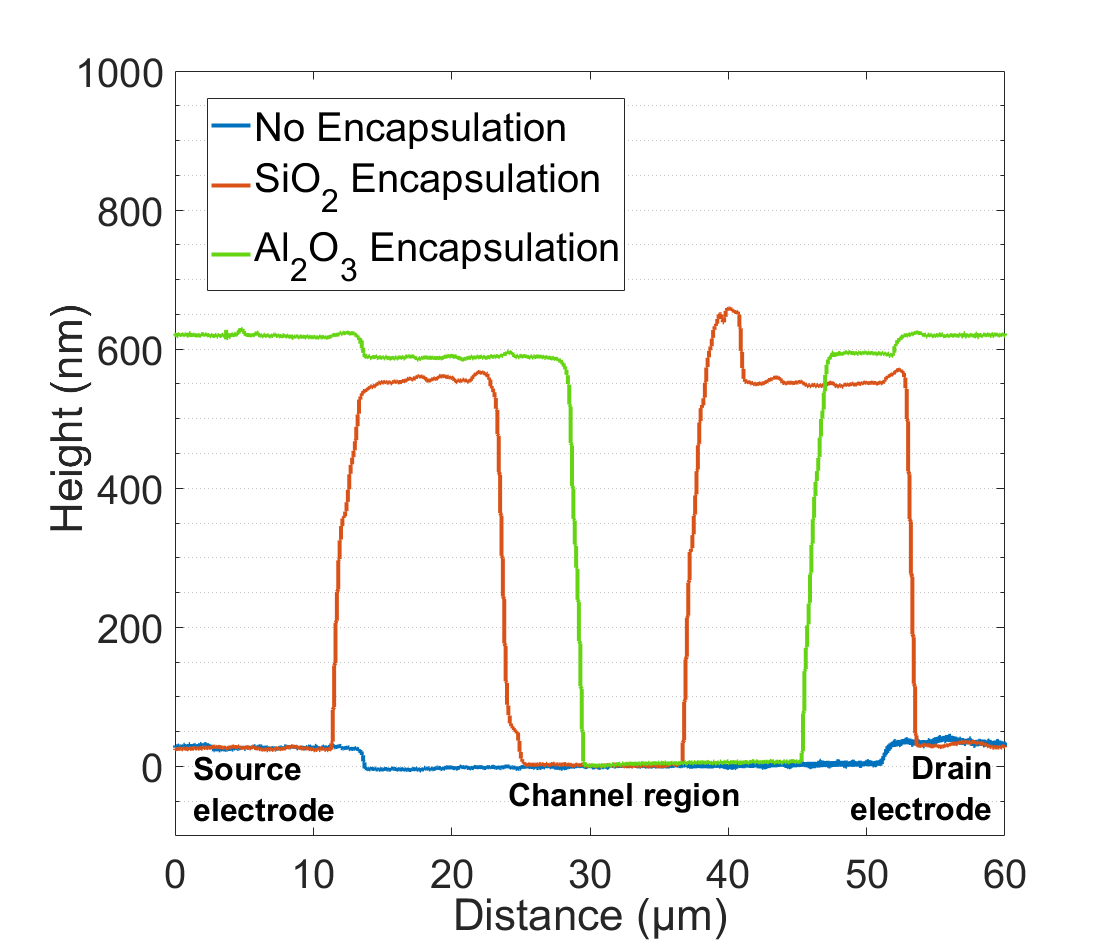
\includegraphics{figures/ch4/Dielectric_Profile_comparison.png}

}

}

\subcaption{\label{fig-dielectric-comparison}}
\end{minipage}%
%
\begin{minipage}[t]{0.05\linewidth}

{\centering 

~

}

\end{minipage}%
%
\begin{minipage}[t]{0.45\linewidth}

{\centering 

\raisebox{-\height}{

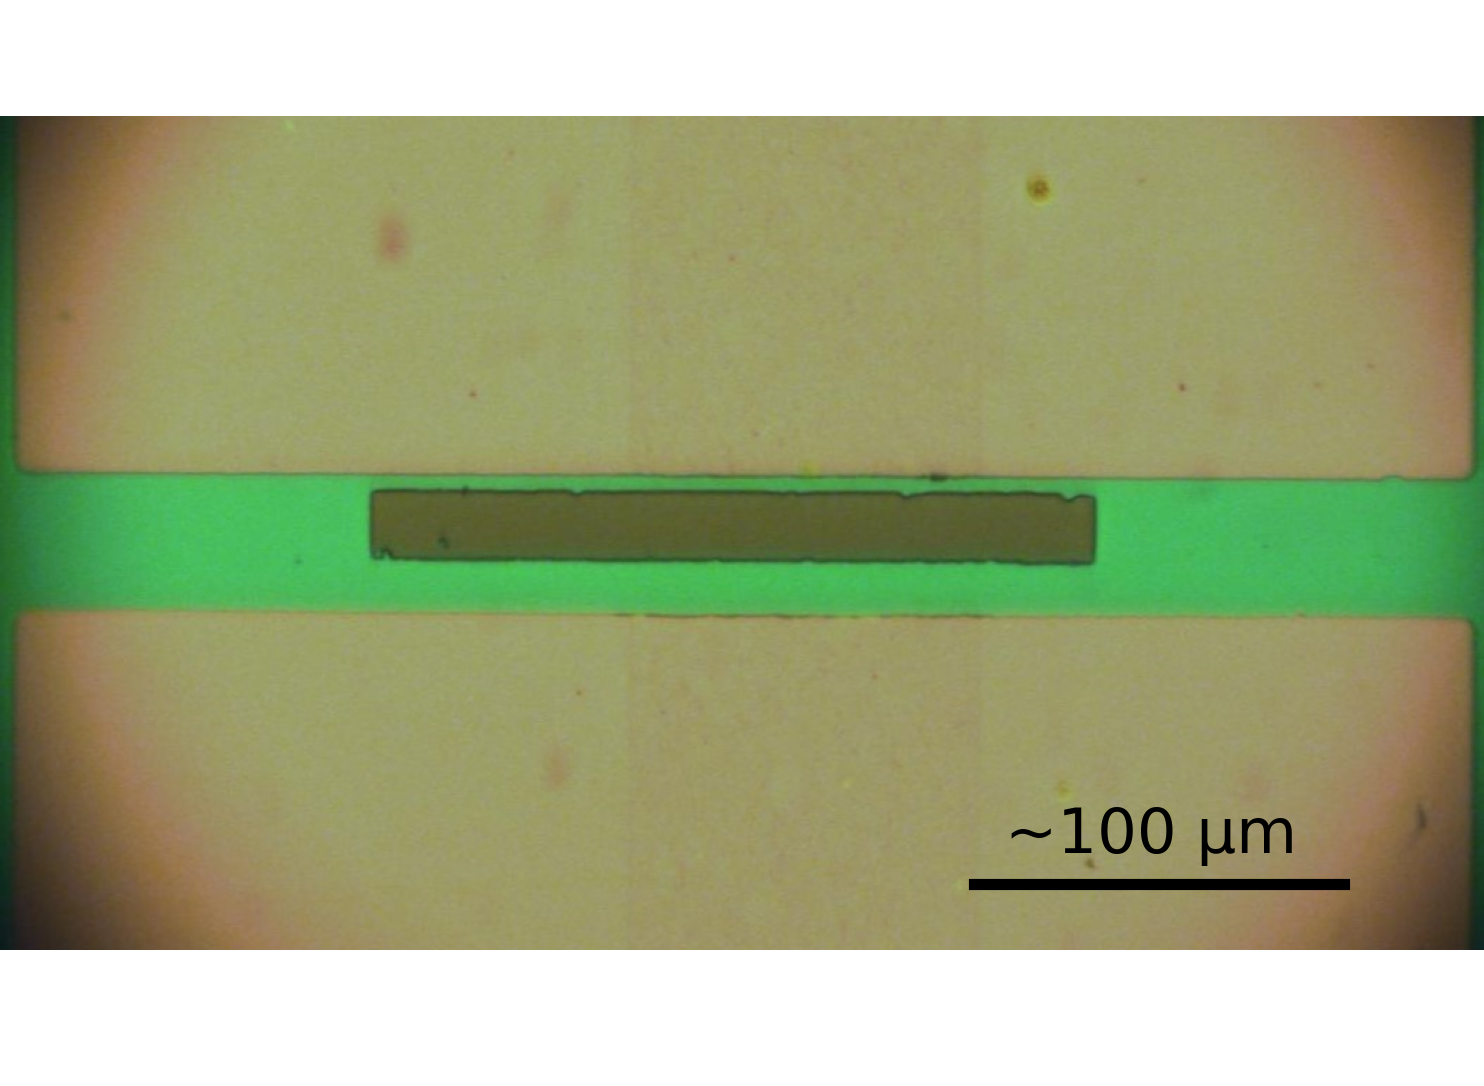
\includegraphics{figures/ch4/al2o3_encapsulation.png}

}

}

\subcaption{\label{fig-al2o3-encapsulation}}
\end{minipage}%

\caption{\label{fig-dektat-dielectric-layer}A profile comparison of
dielectric materials used for encapsulation is shown in (a), alongside a
microscope image of a device encapsulated with aluminium oxide in (b).
Note that the layer thicknesses in (a) were from initial tests of the
process and are used for illustrative purposes.}

\end{figure}

The initial attempt at fabricating a dielectric encapsulation layer used
silicon dioxide as the dielectric. However, silicon dioxide adheres
poorly to gold without an metallic adhesive layer present, as shown in
Figure~\ref{fig-dielectric-comparison}. Aluminium oxide was chosen as an
alternative as it sticks well to bulk electrode materials, is heat and
chemical resistant, has a relatively high dielectric constant and is
bio-compatible \autocite{Guarnieri2014,Albarghouthi2022,Kolodzey2000}.
Figure~\ref{fig-dektat-dielectric-layer} shows the aluminium oxide
successfully adhered to the electrodes and had a clean profile
comparable to that of the SU-8 encapsulation layer after lift-off.

Unfortunately, when aluminium oxide layers which were thicker than
\(\sim\) 100 nm were deposited, there was found to be a significant drop
in current relative to the unencapsulated device. This drop was
signficant enough to make devices unsuitable for sensing. Meanwhile,
devices with encapsulation \(\sim\) 100 nm thick had significant gate
current leakage through the encapsulation layer when liquid-gated. This
leakage was present even when AZ\(^\circledR\) nLOF 2020 was used for
electrode patterning to avoid edge spikes (as discussed in
Section~\ref{sec-electrodes}). Furthermore, aluminium oxide should not
be subsequently exposed to its etchant TMAH, meaning it was difficult to
completely remove residual photoresist from device channels after
encapsulation. Possible future approaches to ceramic encapsulation are
discussed in \textbf{?@sec-future-work}.

\hypertarget{sec-afm-characterisation}{%
\section{Characterisation via Atomic Force
Microscopy}\label{sec-afm-characterisation}}

Atomic force microscopy in this thesis was taken using a Nanosurf
NaioAFM in dynamic force mode (also known as tapping mode, oscillating
mode, acoustic AC mode or intermittent-contact mode). An ACLA probe
(AppNano) was used with a tip diameter of 12 nm, height of \(14-16\)
\(\mu\)m and a nominal cantilever spring constant of 58 N/m. All atomic
force microscopy was performed with the Nanosurf NaioAFM on a stablising
table under a Faraday cage to minimise mechanical and electromagnetic
interference. A 256 \(\times\) 256 pixel resolution was typically used.
Imaging was performed in air at room temperature.

Atomic force microscope (AFM) images could not be taken from the small
exposed channel region on the encapsulated devices, so were instead
taken on a representative carbon nanotube or graphene film sample
fabricated on the same wafer as the device being tested. Moisture
adversely affected the AFM imaging process. Therefore, films
functionalised with biological materials were washed with DI water and
gently dried with N\(_2\) before atomic force microscope images were
taken.

The open source data analysis software Gwyddion (version 2.59) was used
to analyse AFM images. This included levelling the background with the
polynomial background removal function, removing scarring and zeroing
the z-scale.

\hypertarget{sec-fluorescence-characterisation}{%
\section{Characterisation via Fluorescence
Microscopy}\label{sec-fluorescence-characterisation}}

Fluorescence microscopy was performed using an Olympus BX63 fluorescence
microscope controlled using cellSens imaging software. Microscope
objectives used were all Olympus UPLSAPO/UPlanSApo, apochromat
objectives which compensate for spherical and chromatic aberrations.
Objectives had infinite aperture and a field number of 26.5. Filter
cubes used included the Olympus FITC filter (excitation wavelength
range: \(467-498\) nm, emission wavelength range: \(513-556\) nm), Texas
Red (excitation wavelength range: \(542-582\) nm, emission wavelength
range: \(604-644\) nm) and GFP (excitation wavelength range: \(604-644\)
nm, emission wavelength range: \(502-538\) nm). The ISO was kept at the
lowest available setting, ISO200. All microscopy was performed in
darkness with the screen turned away from the microscope. To ensure
photobleaching did not adversely affect imaging, images were taken soon
after initial exposure to fluorescence and taking repeated photos of the
same region was avoided. Various useful and thorough introductions to
fluorescence microscopy can be found online \autocite{Nikon,Zeiss}.

\hypertarget{sec-raman-characterisation}{%
\section{Characterisation via Raman
Spectroscopy}\label{sec-raman-characterisation}}

Raman spectroscopy was performed with a HORIBA Jobin Yvon LabRAM HR800
Raman spectrometer. The wavelength and power used for laser excitation
of samples were 514 nm and 1 mW respectively. Spectra were taken with a
1800 line holographic grating with a hole size of 300 \(\mu\)m. A
accumulation time of 20 seconds was used when taking spectra. Each
spectrum was recorded twice at nine positions on device film, with a
minimum distance of 10 \(\mu\)m between each position. Spectra were
collected over two wavenumber ranges at each position, with the first
range between 100 cm\(^{-1}\) and 650 cm\(^{-1}\), and the second
between 1300 cm\(^{-1}\) and 1650 cm\(^{-1}\).

\hypertarget{sec-electrical-characterisation}{%
\section{Electrical
Characterisation}\label{sec-electrical-characterisation}}

\begin{figure}

{\centering 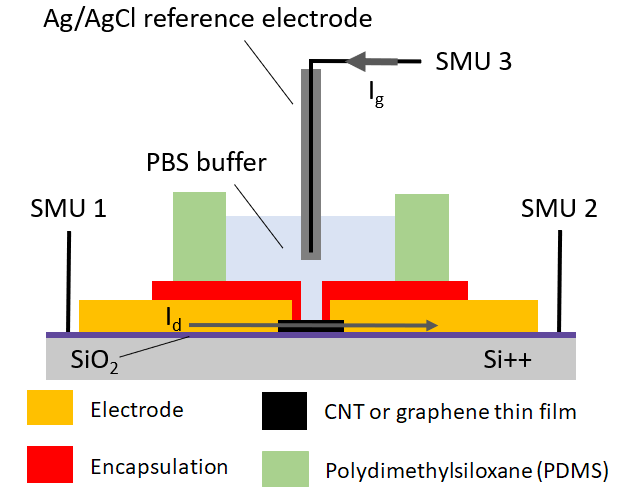
\includegraphics[width=0.9\textwidth,height=\textheight]{figures/ch4/liquid-gate-schematic.png}

}

\caption{\label{fig-liquid-gate-schematic}Liquid-gated device schematic
showing electrical connections to the three source measure units.
V\(_{\mathrm{ds}}\) is applied between the source SMU (SMU 1) and the
drain SMU (SMU 2), while V\(_{\mathrm{lg}}\) is applied between the gate
SMU (SMU 3) and the drain SMU. The drain SMU is held at 0 V or connected
to a ground plane. Drain current I\(_{\mathrm{d}}\) is measured at the
drain SMU, and gate leakage current I\(_{\mathrm{g}}\) is measured at
the gate SMU.}

\end{figure}

Both liquid-gated and back-gated measurements were taken of carbon
nanotube and graphene devices. Liquid-gated measurements were taken
using the configuration shown in Figure~\ref{fig-liquid-gate-schematic}.
Back-gated measurements were taken with a copper plane placed underneath
the Si/SiO\(_2\) wafer and connected to SMU 3 instead of the reference
electrode.

All measurement setups used had the same basic configuration, with two
source measure units (SMUs) attached to the source and gate. Voltage
from the source and gate SMUs was either kept constant or varied, with
only one SMU varied at a time. Three different measurement setups were
used for taking these measurements, the Agilent (Keysight/HP) 4156C
Semiconductor Parameter Analyser, the Keysight B1500A Semiconductor
Device Analyser, and a National Instruments NI-PXIe modular measurement
system with a 8 GB PXIe-8821 controller and two NI-4138 source measure
units. For measurements with the Keysight instruments, a third, drain
SMU was attached and kept at a constant 0 V (as shown in
Figure~\ref{fig-liquid-gate-schematic}).

\begin{figure}

\begin{minipage}[t]{0.25\linewidth}

{\centering 

~

}

\end{minipage}%
%
\begin{minipage}[t]{0.50\linewidth}

{\centering 

\raisebox{-\height}{

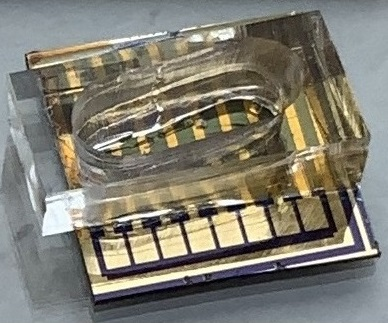
\includegraphics{figures/ch4/IMG_0845_3.jpg}

}

}

\subcaption{\label{fig-PDMS-device-photo}}
\end{minipage}%
%
\begin{minipage}[t]{0.25\linewidth}

{\centering 

~

}

\end{minipage}%
\newline
\begin{minipage}[t]{0.47\linewidth}

{\centering 

\raisebox{-\height}{

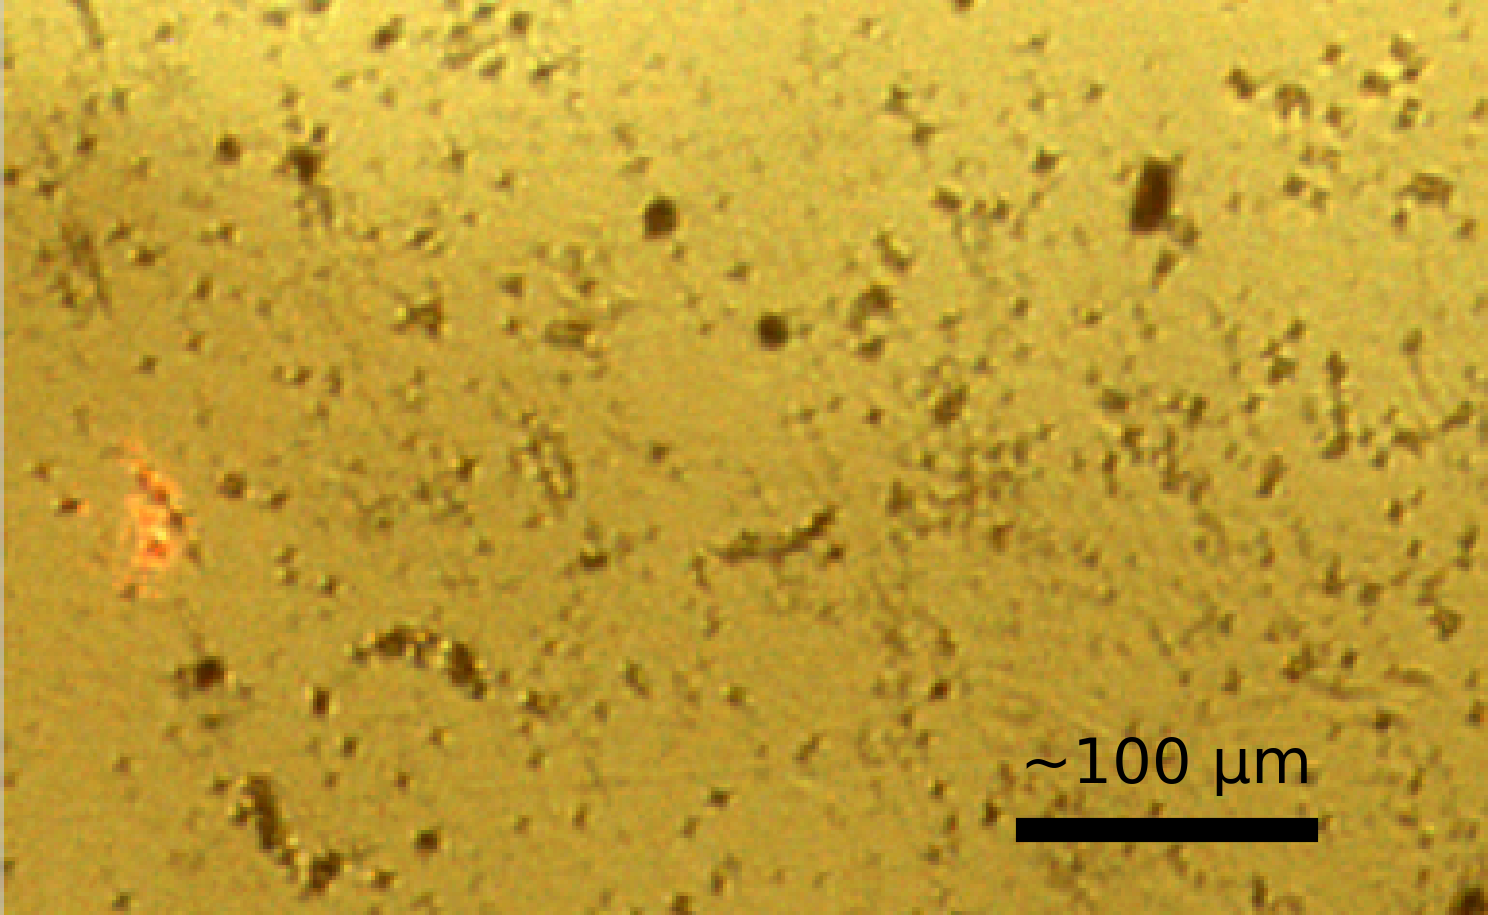
\includegraphics{figures/ch4/PDMS_dirty.png}

}

}

\subcaption{\label{fig-PDMS_dirty}}
\end{minipage}%
%
\begin{minipage}[t]{0.05\linewidth}

{\centering 

~

}

\end{minipage}%
%
\begin{minipage}[t]{0.47\linewidth}

{\centering 

\raisebox{-\height}{

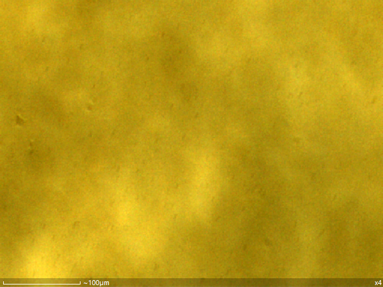
\includegraphics{figures/ch4/PDMS_clean.png}

}

}

\subcaption{\label{fig-PDMS_clean}}
\end{minipage}%

\caption{\label{fig-PDMS-clean}A carbon nanotube field-effect transistor
device with a polydimethylsiloxane (PDMS) `well' placed on the device
surface is seen in (a), followed by microscope images of the surface of
a well before (b) and after (c) isopropanol (IPA) sonication for 10
minutes.}

\end{figure}

When using the Agilent 4156C Semiconductor Parameter Analyser or
Keysight B1500A Semiconductor Device Analyser for liquid-gated
measurements, a Rucker and Kolls with micromanipulators was used to
contact the devices; when using the National Instruments NI-PXIe for
liquid-gated measurements, a custom-made chip carrier with
spring-loaded, pointed-tip, gold-coated pogo pins was used. Ag/AgCl
standard electrodes were used as the liquid-gate electrode. The
electrode was submerged in 80 \(\mu\)L of PBS buffer in a
polydimethylsiloxane (PDMS) `well' \(-\) a flexible structure used to
contain the electrolyte solution \(-\) with outer dimensions of 12 mm
\(\times\) 6 mm \(\times\) 6 mm. This PDMS well was sonicated in
isopropanol for 10 min and thoroughly N\(_2\) dried before use. The
microscope images seen in Figure~\ref{fig-PDMS-clean} show the PDMS
surface before and after this cleaning step. The end of Ag/AgCl standard
electrode to be submerged should be rinsed in DI water and left to sit
in DI water for 15 minutes before characterisation is performed.

The Agilent 4156C Semiconductor Parameter Analyser and Keysight B1500A
Semiconductor Device Analyser were also used for back-gated measurements
of devices within the vapour delivery system device chamber. When the
lid of this chamber was tightly sealed, it acted a Faraday cage for
another custom-made chip carrier with spring-loaded gold-coated pogo
pins, able to contact four channel electrode pairs at once. The silicon
back of the device was pressed by the pins against a copper block,
connected to the gate SMU.

Custom programs for National Instruments LabView 2017 were used for
measurements from the Agilent 4156C Semiconductor Parameter Analyser and
the National Instruments NI-PXIe. Keysight EasyEXPERT software was used
for characterisation with the Keysight B1500A Semiconductor Device
Analyser.

Liquid-gated transfer characteristics of carbon nanotube FETs were
measured at V\(_{\mathrm{ds}}\) = 100 mV and liquid-gated transfer
characteristics of graphene FETs were measured at V\(_{\mathrm{ds}}\) =
1 V, where V\(_{\mathrm{lg}}\) was swept between -0.5 V and 1 V in both
the forward and reverse direction with a step size of either 10 or 20
mV. Backgated transfer characteristics of carbon nanotube FETs were
either measured at V\(_{\mathrm{ds}}\) = 100 mV or V\(_{\mathrm{ds}}\) =
1 V, where V\(_{\mathrm{bg}}\) was swept between -5 V and 5 V or -10 V
and 10 V in the forward and reverse directions with a step size of 50 mV
or 100 mV.

\hypertarget{sensing-measurements}{%
\subsection{Sensing Measurements}\label{sensing-measurements}}

A liquid-gated setup was used for aqueous-phase sensing and a back-gated
setup in the vapour delivery system was used for vapour-phase sensing,
as described above.

Sensing measurements were performed with constant source-drain and gate
voltages. The gate voltage used was chosen by locating the subthreshold
region of the device transfer characteristics and choosing a voltage
that fell within this region, usually V\(_{\mathrm{g}}\) = 0 V.

Using the NI-PXIe with the PXIe-2737 module, eight-channel multiplexed
current measurements could be taken in rapid succession. An integration
time of 200 or 400 ms was used for sampling with each channel, with the
actual sampling rate set by the NI-PXIe. In practice this meant a
sampling rate of 1.81 s (for 200 ms integration time) or 3.41 s (for 400
ms integration time) for any given channel. A 200 ms integration time
meant the time between samples from successive channels varied between
\(220 ms-230\) ms, while a 400 ms integration time meant the time
between samples was consistently 426 ms. The Keysight equipment used a
constant 1 s sampling interval.

\hypertarget{aqueous-sensing}{%
\subsubsection*{Aqueous Sensing}\label{aqueous-sensing}}
\addcontentsline{toc}{subsubsection}{Aqueous Sensing}

Before the sensing process, 200 \(\mu\)L of PBS was added to the PDMS
well and 100-120 \(\mu\)L of PBS was removed. This initial step was
performed to wet the sides of the PDMS well, and check that the
attachment of the PDMS well to the device would not unseal when larger
volumes of PBS were added during sensing. Before any sensing
measurement, a transfer characteristic curve was taken of the
liquid-gated device. The initial amount of buffered electrolyte in the
well was 100\(\mu\)L, unless specified otherwise.

From Feburary 2022 onwards, the standard sensing addition series used
comprised of a `control series' and an `analyte sensing series'. The
control series was performed as part of each sensing experiment to test
for unwanted responses to electrolyte and to allow baseline drift to
settle. The total control series interval was 1800 s. Electrolyte
additions of 20\(\mu\)L were made at 100 s, 200 s and 300 s, while
electrolyte subtractions of 20\(\mu\)L were made at 400 s, 500 s and 600
s. Immediately after the control series, a sensing sequence was
performed as part of the same continuous measurement set. An initial
electrolyte addition was performed at 2100s, to confirm no changes
occurred during the control series that would interfere with sensing.
Unless specified otherwise, five analyte additions were then made with a
time spacing of 300 s, at 2400 s, 2700 s, 3000 s, 3300 s and 3600 s. The
experimental series was set to finish at 4000 s. The exact timings,
analyte concentrations and gate voltage used in a given sensing sequence
are discussed alongside the relevant experimental results.

\hypertarget{vapour-sensing}{%
\subsubsection*{Vapour Sensing}\label{vapour-sensing}}
\addcontentsline{toc}{subsubsection}{Vapour Sensing}

A variety of vapour sensing sequences were used in this work, which are
discussed in \textbf{?@sec-vapour-sensing-biosensors} in detail.

\hypertarget{summary}{%
\section{Summary}\label{summary}}

A variety of approaches were trialled when depositing a carbon nanotube
network for the fabrication of transistor devices, and the resulting
morphologies of these networks are discussed in the next chapter.
Standard photolithographic methods were used to successfully fabricate
carbon nanotube and graphene field effect transistor devices. A range of
photolithography types and electrode/encapsulation materials were
trialled to find the optimal device composition for sensing, also
discussed in the next chapter. Atomic force microscopy, fluorescence
microscopy and a variety of electrical measurement setups were used to
characterise the devices.

\bookmarksetup{startatroot}

\hypertarget{characteristics-of-pristine-carbon-nanotube-graphene-field-effect-transistors}{%
\chapter{Characteristics of Pristine Carbon Nanotube \& Graphene Field
Effect
Transistors}\label{characteristics-of-pristine-carbon-nanotube-graphene-field-effect-transistors}}

\hypertarget{introduction-1}{%
\section{Introduction}\label{introduction-1}}

A range of methods were followed to fabricate carbon nanotube network
and graphene field-effect transistors for biosensor use. This chapter
therefore looks to use the characterisation techniques outlined in the
previous chapter to compare and contrast the device channel morphologies
and electrical characteristics resulting from various methods.

The three carbon nanotube film types used for devices were the
solvent-deposited, surfactant-deposited and steam-assisted
surfactant-deposited (steam-deposited) films discussed in the previous
chapter. As minor changes were made to fabrication processes throughout
the thesis, the fabrication dates of devices used are stated, which can
be cross-referenced with Chapter~\ref{sec-fabrication} to identify the
specific process used. Atomic force microscopy and Raman spectroscopy
was performed on the carbon nanotube networks to identify the
distribution of carbon nanotube diameters and the defects present on the
carbon nanotube networks. Electrical characterisation was then used to
see how the morphology of each film type affects the performance of the
completed devices. Both back-gated and liquid-gated transfer
characteristics were compared, as well as key parameters taken from the
liquid-gated characteristics. The electrical behaviour of liquid-gated
graphene devices was also examined, as well as the impact of water on
the performance of back-gated devices for vapour sensing use.

Finally, as a control measurement for liquid-gated sensing and to verify
the behaviour of the pristine device as a sensor, a salt concentration
sensing series was performed with a steam-deposited carbon nanotube
network device. The device characteristics were taken and device drift
was examined and modelled. The sensing series was performed by
successively diluting 1XPBS electrolyte in the polydimethylsiloxane
`well' (electrolyte container) while passing a current through the
device, and measuring the current response to dilutions. Various filters
were applied to the collected data to better understand the signal
change.

\hypertarget{sec-pristine-morphology}{%
\section{Carbon Nanotube Network Morphology and
Composition}\label{sec-pristine-morphology}}

\hypertarget{sec-pristine-AFM}{%
\subsection{Atomic Force Microscopy}\label{sec-pristine-AFM}}

Figure~\ref{fig-afm-morphology} shows a side-by-side comparison of the
surface morphology of carbon nanotube films fabricated using the methods
described in Section~\ref{sec-dep-carbon-nanotubes}. These images were
collected using an atomic force microscope and processed in the manner
described in Section~\ref{sec-afm-characterisation}.
Figure~\ref{fig-bundled-network} shows a film of carbon nanotubes
deposited in solvent, Figure~\ref{fig-dropcast-network} shows a film of
carbon nanotubes dropcast in surfactant, and
Figure~\ref{fig-steaming-network} shows carbon nanotubes dropcast in
surfactant in the presence of steam. As discussed in previous works
using solvent-based deposition techniques for depositing carbon
nanotubes, in each network multi-tube bundles form due to strong mutual
attraction between nanotubes
\autocite{Zheng2017,Murugathas2018,Murugathas2019a,Nguyen2021}. However,
when surfactants are present, they adsorb onto the carbon nanotubes and
form a highly repulsive structure able to overcome the strong attraction
between nanotubes. This repulsion keeps the individual carbon nanotubes
more isolated
\autocite{Wenseleers2004,Gavrel2013,Hermanson2013-16,Shimizu2013,DiCrescenzo2014}.
The diameter range provided by the supplier for the individual carbon
nanotubes used is \(1.2-1.7\) nm, while the length range is \(0.3-5.0\)
\(\mu\)m (Nanointegris).

\begin{figure}

\begin{minipage}[t]{0.47\linewidth}

{\centering 

\raisebox{-\height}{

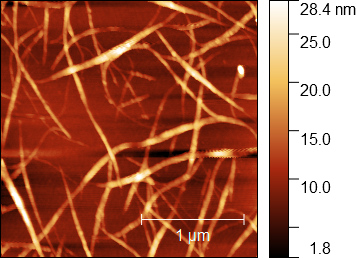
\includegraphics{figures/ch5/Ned_NTQ24_20220125_00235.png}

}

}

\subcaption{\label{fig-bundled-network}}
\end{minipage}%
%
\begin{minipage}[t]{0.05\linewidth}

{\centering 

~

}

\end{minipage}%
%
\begin{minipage}[t]{0.47\linewidth}

{\centering 

\raisebox{-\height}{

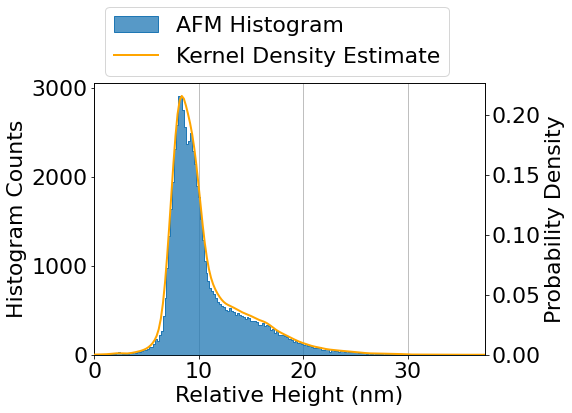
\includegraphics{figures/ch5/Ned_NTQ24_20220125_00235_histogram_initialguess.png}

}

}

\subcaption{\label{fig-bundled-network-histogram}}
\end{minipage}%
\newline
\begin{minipage}[t]{0.47\linewidth}

{\centering 

\raisebox{-\height}{

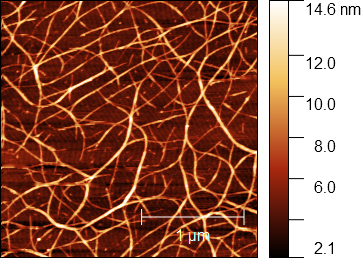
\includegraphics{figures/ch5/Ned_NTQ8C7_w4_pristine_00084_20210428(2).png}

}

}

\subcaption{\label{fig-dropcast-network}}
\end{minipage}%
%
\begin{minipage}[t]{0.05\linewidth}

{\centering 

~

}

\end{minipage}%
%
\begin{minipage}[t]{0.47\linewidth}

{\centering 

\raisebox{-\height}{

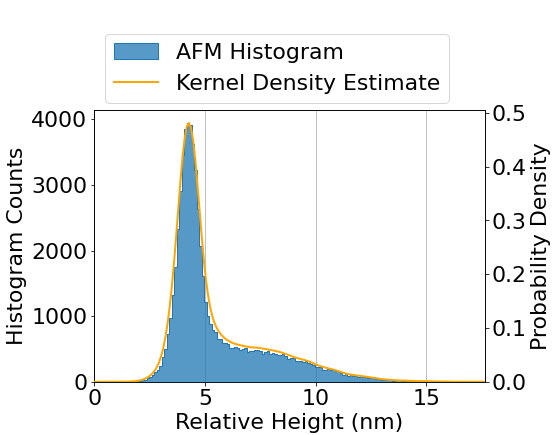
\includegraphics{figures/ch5/Ned_NTQ8C7_w4_pristine_00084_20210428(2)_histogram_initialguess.png}

}

}

\subcaption{\label{fig-dropcast-network-histogram}}
\end{minipage}%
\newline
\begin{minipage}[t]{0.47\linewidth}

{\centering 

\raisebox{-\height}{

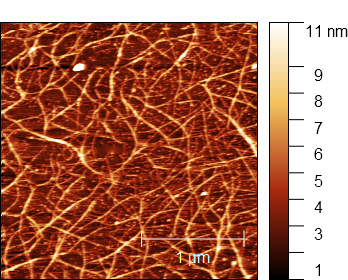
\includegraphics{figures/ch5/Ned_NGQ14D2_W4_pristine_20220713_00567.png}

}

}

\subcaption{\label{fig-steaming-network}}
\end{minipage}%
%
\begin{minipage}[t]{0.05\linewidth}

{\centering 

~

}

\end{minipage}%
%
\begin{minipage}[t]{0.47\linewidth}

{\centering 

\raisebox{-\height}{

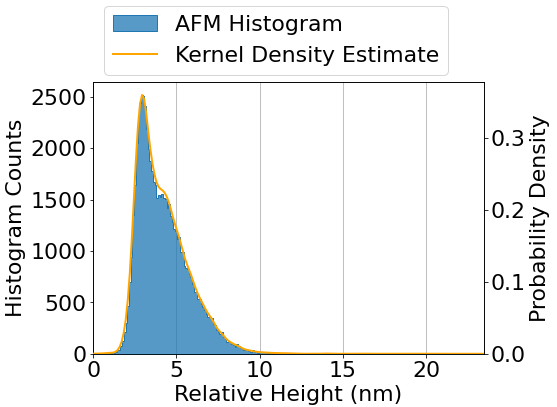
\includegraphics{figures/ch5/Ned_NGQ14D2_W4_pristine_20220713_00567_histogram_initialguess.png}

}

}

\subcaption{\label{fig-steaming-network-histogram}}
\end{minipage}%

\caption{\label{fig-afm-morphology}2.5 \(\mu\)m \(\times\) 2.5 \(\mu\)m
atomic force microscope (AFM) images of carbon nanotube films deposited
using various methods, shown side-by-side with histogram height
distributions and kernel density estimate (KDE) plots corresponding to
each image. The network shown in (a) with height distribution shown in
(b) was deposited in solvent, the network shown in (c) with height
distribution shown in (d) was dropcast in surfactant, and the network
shown in (e) with height distribution shown in (f) was dropcast in
surfactant with steam present.}

\end{figure}

It has previously been demonstrated that the diameter range of deposited
single-walled carbon nanotubes can be modelled via a normal or Gaussian
distribution \autocite{LeMieux2008,Liu2013,Vobornik2023}. However, when
we directly extract and bin the height profiles from the 2.5 \(\mu\)m
\(\times\) 2.5 \(\mu\)m AFM images, plotted in black in
Figure~\ref{fig-afm-morphology}, we obtain histograms which do not
follow a normal distribution. One reason for this result is the surface
roughness of the silicon dioxide substrate. The carbon nanotubes do not
lie perfectly level on a perfectly level silicon oxide substrate. In
practice, both the SiO\(_2\) substrate and the surface of the carbon
nanotubes both have a degree of roughness. To find the contribution of
surface roughness to the height profile histogram corresponding to each
network deposition method, silicon dioxide substrates were modified
using the same processes as in Figure~\ref{fig-afm-morphology} but
without carbon nanotubes present in the solutions used. 2.5 \(\mu\)m
\(\times\) 2.5 \(\mu\)m AFM images of the modified surfaces are shown in
Figure~\ref{fig-afm-substrate}.

\begin{figure}

\begin{minipage}[t]{0.47\linewidth}

{\centering 

\raisebox{-\height}{

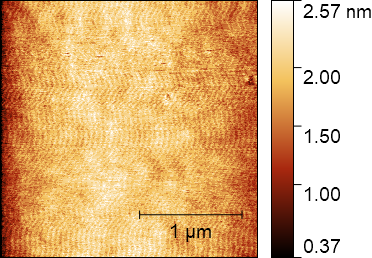
\includegraphics{figures/ch5/Ned_SiO2_00351_20231016.png}

}

}

\subcaption{\label{fig-sio2-only}}
\end{minipage}%
%
\begin{minipage}[t]{0.05\linewidth}

{\centering 

~

}

\end{minipage}%
%
\begin{minipage}[t]{0.47\linewidth}

{\centering 

\raisebox{-\height}{

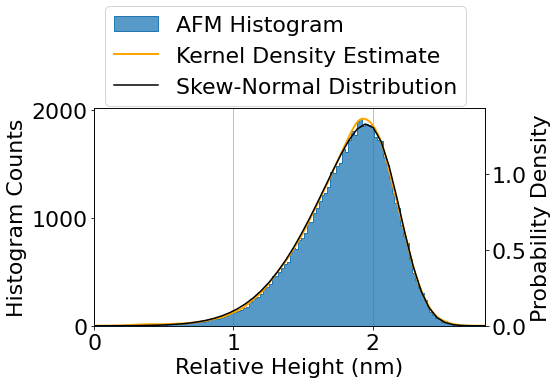
\includegraphics{figures/ch5/Ned_SiO2_00351_20231016_histogram_initialguess.png}

}

}

\subcaption{\label{fig-sio2-histogram}}
\end{minipage}%
\newline
\begin{minipage}[t]{0.47\linewidth}

{\centering 

\raisebox{-\height}{

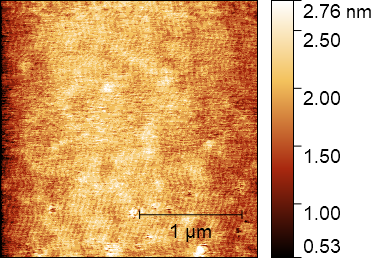
\includegraphics{figures/ch5/Ned_SiO2_s_surfactant_nosteam_00355_20231016.png}

}

}

\subcaption{\label{fig-surfactant-afm}}
\end{minipage}%
%
\begin{minipage}[t]{0.05\linewidth}

{\centering 

~

}

\end{minipage}%
%
\begin{minipage}[t]{0.47\linewidth}

{\centering 

\raisebox{-\height}{

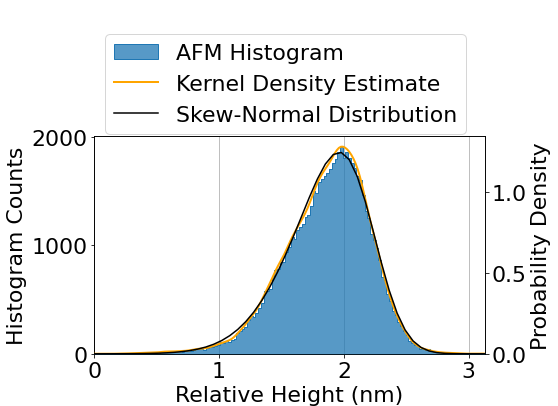
\includegraphics{figures/ch5/Ned_SiO2_s_surfactant_nosteam_00355_20231016_histogram_initialguess.png}

}

}

\subcaption{\label{fig-surfactant-histogram}}
\end{minipage}%
\newline
\begin{minipage}[t]{0.47\linewidth}

{\centering 

\raisebox{-\height}{

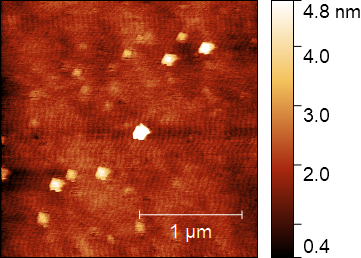
\includegraphics{figures/ch5/Ned_SiO2_s_surfactant_steam_00357_20231016.png}

}

}

\subcaption{\label{fig-steamed-surfactant}}
\end{minipage}%
%
\begin{minipage}[t]{0.05\linewidth}

{\centering 

~

}

\end{minipage}%
%
\begin{minipage}[t]{0.47\linewidth}

{\centering 

\raisebox{-\height}{

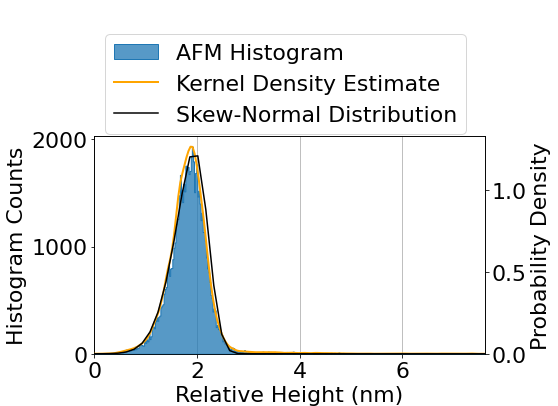
\includegraphics{figures/ch5/Ned_SiO2_s_surfactant_steam_00357_20231016_histogram_initialguess.png}

}

}

\subcaption{\label{fig-steamed-surfactant-histogram}}
\end{minipage}%

\caption{\label{fig-afm-substrate}2.5 \(\mu\)m \(\times\) 2.5 \(\mu\)m
atomic force microscope (AFM) images of silicon dioxide substrates
alongside histogram height distributions and KDE plots corresponding to
each image. The substrate in (a) and (b) was exposed to solvent, the
substrate in (c) and (d) was exposed to surfactant, and the substrate in
(e) and (f) was exposed to surfactant with steam present.}

\end{figure}

In Figure~\ref{fig-afm-substrate}, we see that each substrate surface
has a roughness that follows a normal distribution with some degree of
skewness. Figure~\ref{fig-sio2-histogram} and
Figure~\ref{fig-surfactant-histogram} are negatively skewed
distributions. The fitted skew-normal distribution in
Figure~\ref{fig-sio2-histogram} has a skew parameter \(\alpha\) (or
shape parameter) of -3.2, a location parameter \(\xi\) of 2.2 nm and a
scale parameter \(\omega\) of 0.5 nm, while in
Figure~\ref{fig-surfactant-histogram} \(\alpha = -2.2\), \(\xi = 2.2\)
nm and \(\omega = 0.5\) nm. \(\xi\) and \(\omega\) correspond to the
mean and standard deviation of the skew-free normal distribution when
\(\alpha\) is set equal to zero \autocite{Azzalini1999}. The close
correspondence between \(\xi\) and \(\omega\) for these distributions
but not \(\alpha\) implies that the skewness is a variable imaging or
processing artifact rather than a physical property of the surface.
Without distortion, the roughness of a clean SiO\(_2\) surface should
follow a normal distribution \autocite{Velicky2015}.

However, Figure~\ref{fig-steamed-surfactant-histogram} has a pronounced
positive skew with a long tail. The tail appears to result from the
contribution of residual surfactant aggregates to surface morphology,
observed in Figure~\ref{fig-steamed-surfactant} and recently discussed
elsewhere in the literature \autocite{Christensen2022,Vobornik2023}.
Attempting to fit a skew-normal distribution to this histogram fails
when all three variables are allowed to vary due to the presence of the
tail. Instead, we fix \(\xi\) and \(\omega\) at 2.2 nm and 0.5 nm
respectively to mimic the silicon dioxide distributions previously
obtained, and only \(\alpha\) is allowed to vary during the fitting
process. The result is shown in
Figure~\ref{fig-steamed-surfactant-histogram}. The fitted distribution
has an \(\alpha\) of -2.4. The distribution closely fits the negative
tail of the histogram, but deviates slightly from the positive tail due
to the presence of surfactant. Since this deviation is small, the
quality of the fit is still reasonably high, with an R-squared value of
0.98. Surfactant contamination could have negative effects on both
sensitivity of carbon nanotubes and also could damage attached
biological elements.

\begin{figure}

\begin{minipage}[t]{0.47\linewidth}

{\centering 

\raisebox{-\height}{

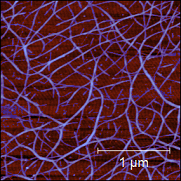
\includegraphics{figures/ch5/Ned_NTQ8C7_w4_pristine_00084_20210428(2)_mask.png}

}

}

\subcaption{\label{fig-mask}}
\end{minipage}%
%
\begin{minipage}[t]{0.05\linewidth}

{\centering 

~

}

\end{minipage}%
%
\begin{minipage}[t]{0.47\linewidth}

{\centering 

\raisebox{-\height}{

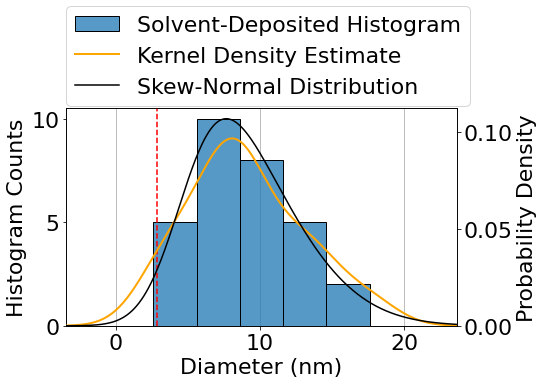
\includegraphics{figures/ch5/NTQ24_20220125_00235_cnt_histogram.png}

}

}

\subcaption{\label{fig-solvent-cnt-histogram}}
\end{minipage}%
\newline
\begin{minipage}[t]{0.47\linewidth}

{\centering 

\raisebox{-\height}{

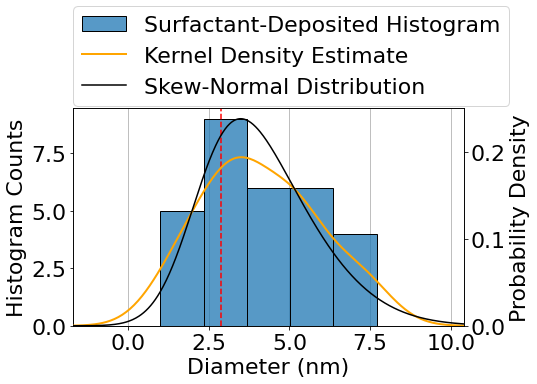
\includegraphics{figures/ch5/NTQ8C7_w4_pristine_cnt_histogram.png}

}

}

\subcaption{\label{fig-surfactant-cnt-histogram}}
\end{minipage}%
%
\begin{minipage}[t]{0.05\linewidth}

{\centering 

~

}

\end{minipage}%
%
\begin{minipage}[t]{0.47\linewidth}

{\centering 

\raisebox{-\height}{

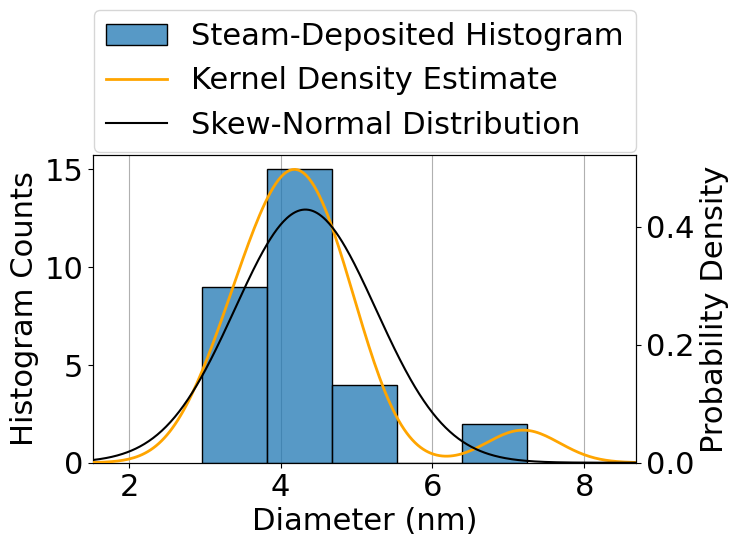
\includegraphics{figures/ch5/NT14D2_W4_pristine_cnt_histogram.png}

}

}

\subcaption{\label{fig-steamed-surfactant-cnt-histogram}}
\end{minipage}%

\caption{\label{fig-cnt-histogram}An masked AFM image is shown in (a),
where the masked carbon nanotube bundles are shaded blue. The mask sets
a height threshold so that masked features are excluded from the height
dataset. Histogram height distributions with corresponding KDE plots
collected via the morphology analysis method outlined by Vobornik
\emph{et al.} \autocite{Vobornik2023} are shown in (b)-(d). The
substrate in (b) was exposed to solvent, the substrate in (c) was
exposed to surfactant, and the substrate in (d) was exposed to
surfactant with steam present.}

\end{figure}

Using the morphology analysis technique outlined by Vobornik \emph{et
al.} \autocite{Vobornik2023}, we collected five successive diameter
measurements of 30 carbon nanotube bundles using Gwyddion. Measurements
were not taken at bundle junctions. A height threshold `mask' was
defined in Gwyddion to determine average substrate height, as shown in
Figure~\ref{fig-mask}. This background value was subtracted from our
diameter measurements to determine the actual bundle height. The means
of the solvent-deposited, surfactant-deposited and steam-assisted
surfactant-deposited bundle diameter histograms are \(8.8 \pm 4.0\) nm,
\(4.2 \pm 1.8\) nm and \(3.3 \pm 1.0\) nm respectively. We see that an
increased maximum feature height leads to an increased mean background
height, and by examining the AFM images in
Figure~\ref{fig-afm-morphology} we see that this may be due to deep
artifacts on the surface of the substrate in the vicinity of large
features. The average of the five height-adjusted values for each carbon
nanotube bundle was then calculated, and these 30 averages were sorted
into six equal-sized bins. The binned bundle diameter measurements,
alongside estimated probability density, are shown in
Figure~\ref{fig-cnt-histogram}.

We notice from Figure~\ref{fig-cnt-histogram} that each histogram
appears to follow a positively skewed normal distribution, different to
the skew-free normal distribution we expect from previous works
\autocite{LeMieux2008,Liu2013,Vobornik2023}. The skew is likely another
artifact from imaging the network with the atomic force microscope. The
force of the atomic force microscope tip is known to cause larger
bundles to undergo some degree of compression, and the resulting
systematic underestimation of their height may be responsible for the
distribution skewness \autocite{Vobornik2023}. The fitted skew-normal
distribution in Figure~\ref{fig-solvent-cnt-histogram} has
\(\alpha = 2.7\), \(\xi = 4.3\) nm, \(\omega = 5.9\) nm, the
distribution in Figure~\ref{fig-surfactant-cnt-histogram} has
\(\alpha = 2.4\), \(\xi = 2.2\) nm, \(\omega = 2.6\) nm, and the
distribution in Figure~\ref{fig-steamed-surfactant-cnt-histogram} has
\(\alpha = 3.6\), \(\xi = 2.2\) nm and \(\omega = 1.5\) nm. We notice
that the probability density for the carbon nanotube bundle histogram
drops to approximately zero at or before 0 nm, as is physically
appropriate.

\hypertarget{tbl-circle-packing}{}
\begin{longtable}[]{@{}
  >{\raggedright\arraybackslash}p{(\columnwidth - 16\tabcolsep) * \real{0.1053}}
  >{\raggedright\arraybackslash}p{(\columnwidth - 16\tabcolsep) * \real{0.1228}}
  >{\raggedright\arraybackslash}p{(\columnwidth - 16\tabcolsep) * \real{0.0965}}
  >{\raggedright\arraybackslash}p{(\columnwidth - 16\tabcolsep) * \real{0.0965}}
  >{\raggedright\arraybackslash}p{(\columnwidth - 16\tabcolsep) * \real{0.1228}}
  >{\raggedright\arraybackslash}p{(\columnwidth - 16\tabcolsep) * \real{0.1228}}
  >{\raggedright\arraybackslash}p{(\columnwidth - 16\tabcolsep) * \real{0.1228}}
  >{\raggedright\arraybackslash}p{(\columnwidth - 16\tabcolsep) * \real{0.1228}}
  >{\raggedright\arraybackslash}p{(\columnwidth - 16\tabcolsep) * \real{0.0877}}@{}}
\caption{\label{tbl-circle-packing}The first eight optimised ratios of
2D packed circle diameter to encompassing circle diameter, given to 3
s.f. (encompassing circle diameter = \(d\), number of packed circles =
\(n\), approximate packed circle diameter = \(d_n\)).\\
}\tabularnewline
\toprule\noalign{}
\endfirsthead
\endhead
\bottomrule\noalign{}
\endlastfoot
\(n\) & \text{2} & \text{3} & \text{4} & \text{5} & \text{6} & \text{7}
& \text{8} & \text{9} \\
\(d\)/\(d_n\) & \text{2.00} & 2.15 & 2.41 & \text{2.70} & \text{3.00} &
\text{3.00} & \text{3.30} & 3.61 \\
\end{longtable}

If we model carbon nanotube bundles as cylinders, and we assume the
component nanotubes follow 2D packing and are of equal diameter, we can
state the mean bundle size for each deposition type in terms of number
of nanotubes \emph{n} \autocite{Graham1998,Murugathas2018,Specht2023}.
Table~\ref{tbl-circle-packing} shows the relationship between the
diameter of a bundle and the constituent diameters of up to nine 2D
packed carbon nanotubes within that bundle. Assuming an average carbon
nanotube diameter of 1.45 nm, we can use the \(d\)/\(d_n\) packing
ratios to obtain an estimate of the number of nanotubes in the mean
bundle size for each deposition \autocite{Specht2023}. These estimates
are shown in Table~\ref{tbl-histogram-parameters}. Also shown in
Table~\ref{tbl-histogram-parameters} is an estimate of the ratio of
single- to multi-tube bundles for each deposition. This estimate was
obtained by taking the integral of each distribution with a lower bound
of 2.9 nm, the minimum multi-tube bundle size for 1.45 nm diameter
nanotubes. As the area under the curve represents the probability a
bundle will have a particular diameter, this integral should give a good
estimate of the relative proportion of multi-tube bundles.
Table~\ref{tbl-histogram-parameters} should be interpreted as
lower-limit estimates of the size and relative proportion of bundles,
recalling that the distribution skewness indicates underestimation of
the true bundle height.

\hypertarget{tbl-histogram-parameters}{}
\begin{table}
\caption{\label{tbl-histogram-parameters}The mean of histogram distributions for carbon nanotube films deposited
using various methods, alongside estimates for the number of nanotubes
present per mean bundle and the estimated proportion of multi-tubed
bundles present across the network. }\tabularnewline

\centering
\begin{tabular}{>{\raggedright\arraybackslash}p{4cm}>{\centering\arraybackslash}p{3cm}>{\centering\arraybackslash}p{3cm}>{\centering\arraybackslash}p{3cm}}
\toprule
 & Mean Bundle Diameter (nm) & Tubes per Average Bundle & \% Multi-Tube Bundles\\
\midrule
Solvent deposited & 8.8 ± 4.0 & 28 & > 96\%\\
Surfactant deposited & 4.2 ± 1.8 & 5 & > 75\%\\
Surfactant deposited with steam & 3.3 ± 1.0 & 3 & > 65\%\\
\bottomrule
\end{tabular}
\end{table}

Both the carbon nanotube bundle diameter mean and standard deviation are
small for surfactant-deposited films when compared to the mean and
standard deviation of solvent-deposited films. However, despite the
presence of surfactant, it is apparent both from
Figure~\ref{fig-afm-morphology} and Table~\ref{tbl-histogram-parameters}
that not all surfactant-dispersed carbon nanotubes are deposited
individually. Bundling may occur during the process of deposition onto
the substrate, which could disrupt the repulsive forces from the
surfactant coating and allow attractive forces to temporarily dominate.
It is possible that the bundling of surfactant-dispersed carbon
nanotubes is a consequence of dynamics introduced by the coffee-ring
effect \autocite{Deegan1997,VanGaalen2021}. The coffee-ring effect
refers to a build-up of dispersed solid forming around the edges of a
dispersion evaporating on a surface. This process occurs due to the
dispersion edges being fixed by surface forces, leading to capillary
flow outwards to replace liquid evaporating at the edges, bringing solid
material along with it. The presence of vapour is known to disrupt this
capillary effect \autocite{Bishop2020}, which may explain why mean
bundle diameter is lower for the films deposited in surfactant with
steam present relative to films deposited in surfactant without steam.

From this discussion, we can conclude that the histograms shown in
Figure~\ref{fig-afm-morphology} are linear combinations of skewed normal
distributions corresponding to both the substrate surface, with a
negative skew, and the carbon nanotube bundles, with a positive skew. X
and Y junctions between overlapping nanotubes may also form a similarly
skewed normal distribution as part of the full histogram
\autocite{Murugathas2018}. The complete linear combination could be
modelled mathematically in order to rapidly extract key parameters from
atomic force microscope images \autocite{Marchenko2010}, but
implementing this approach is outside of the scope of this thesis. The
prevalence of carbon nanotube bundling on the surface is lowered by the
presence of surfactant during deposition. Introducing steam when
depositing with surfactant lowers bundling even further, but also leads
to residual surfactant pooling and attaching to the substrate surface.
These results may both be explained by the presence of steam enabling
surfactant to follow carbon nanotubes to the substrate surface, which
keeps them from bundling during the attachment process. The unwanted
persistence of surfactant means that higher temperature vacuum annealing
may be required for robust biosensors \autocite{Kane2014}.

\hypertarget{sec-pristine-raman}{%
\subsection{Raman Spectroscopy}\label{sec-pristine-raman}}

\begin{figure}

\begin{minipage}[t]{0.47\linewidth}

{\centering 

\raisebox{-\height}{

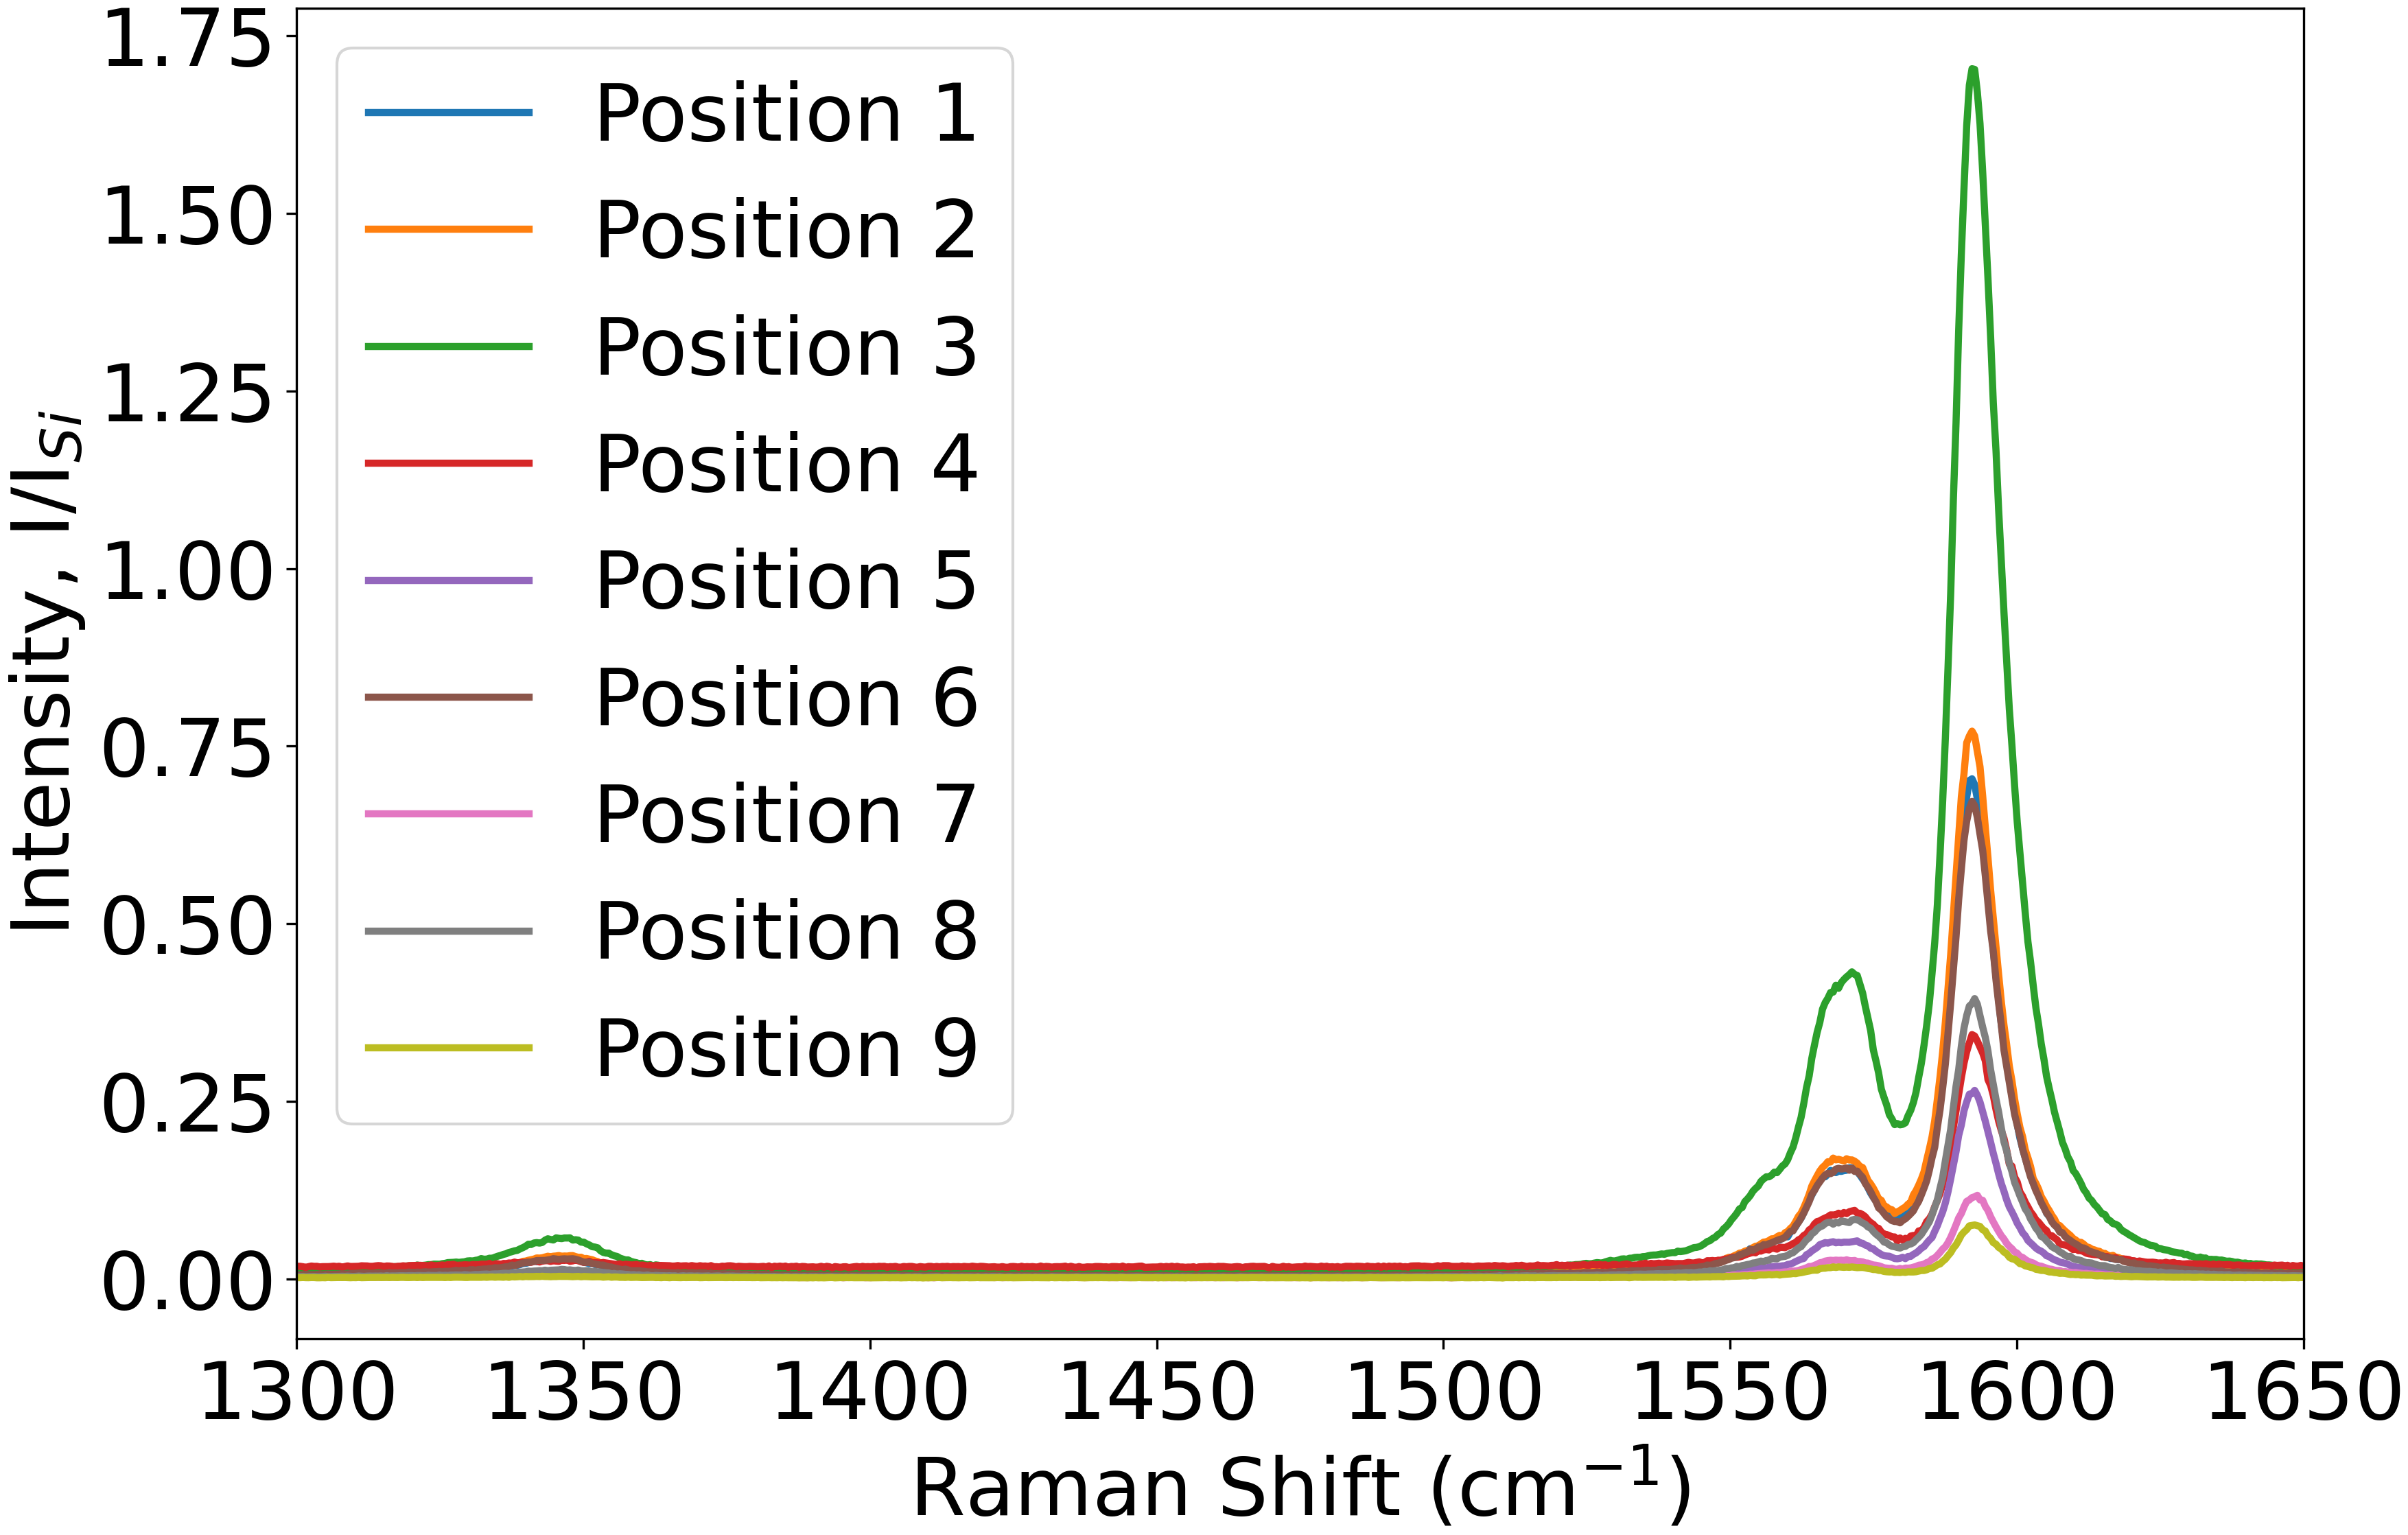
\includegraphics{figures/ch5/bundled_raman.png}

}

}

\subcaption{\label{fig-solvent-deposited}}
\end{minipage}%
%
\begin{minipage}[t]{0.05\linewidth}

{\centering 

~

}

\end{minipage}%
%
\begin{minipage}[t]{0.47\linewidth}

{\centering 

\raisebox{-\height}{

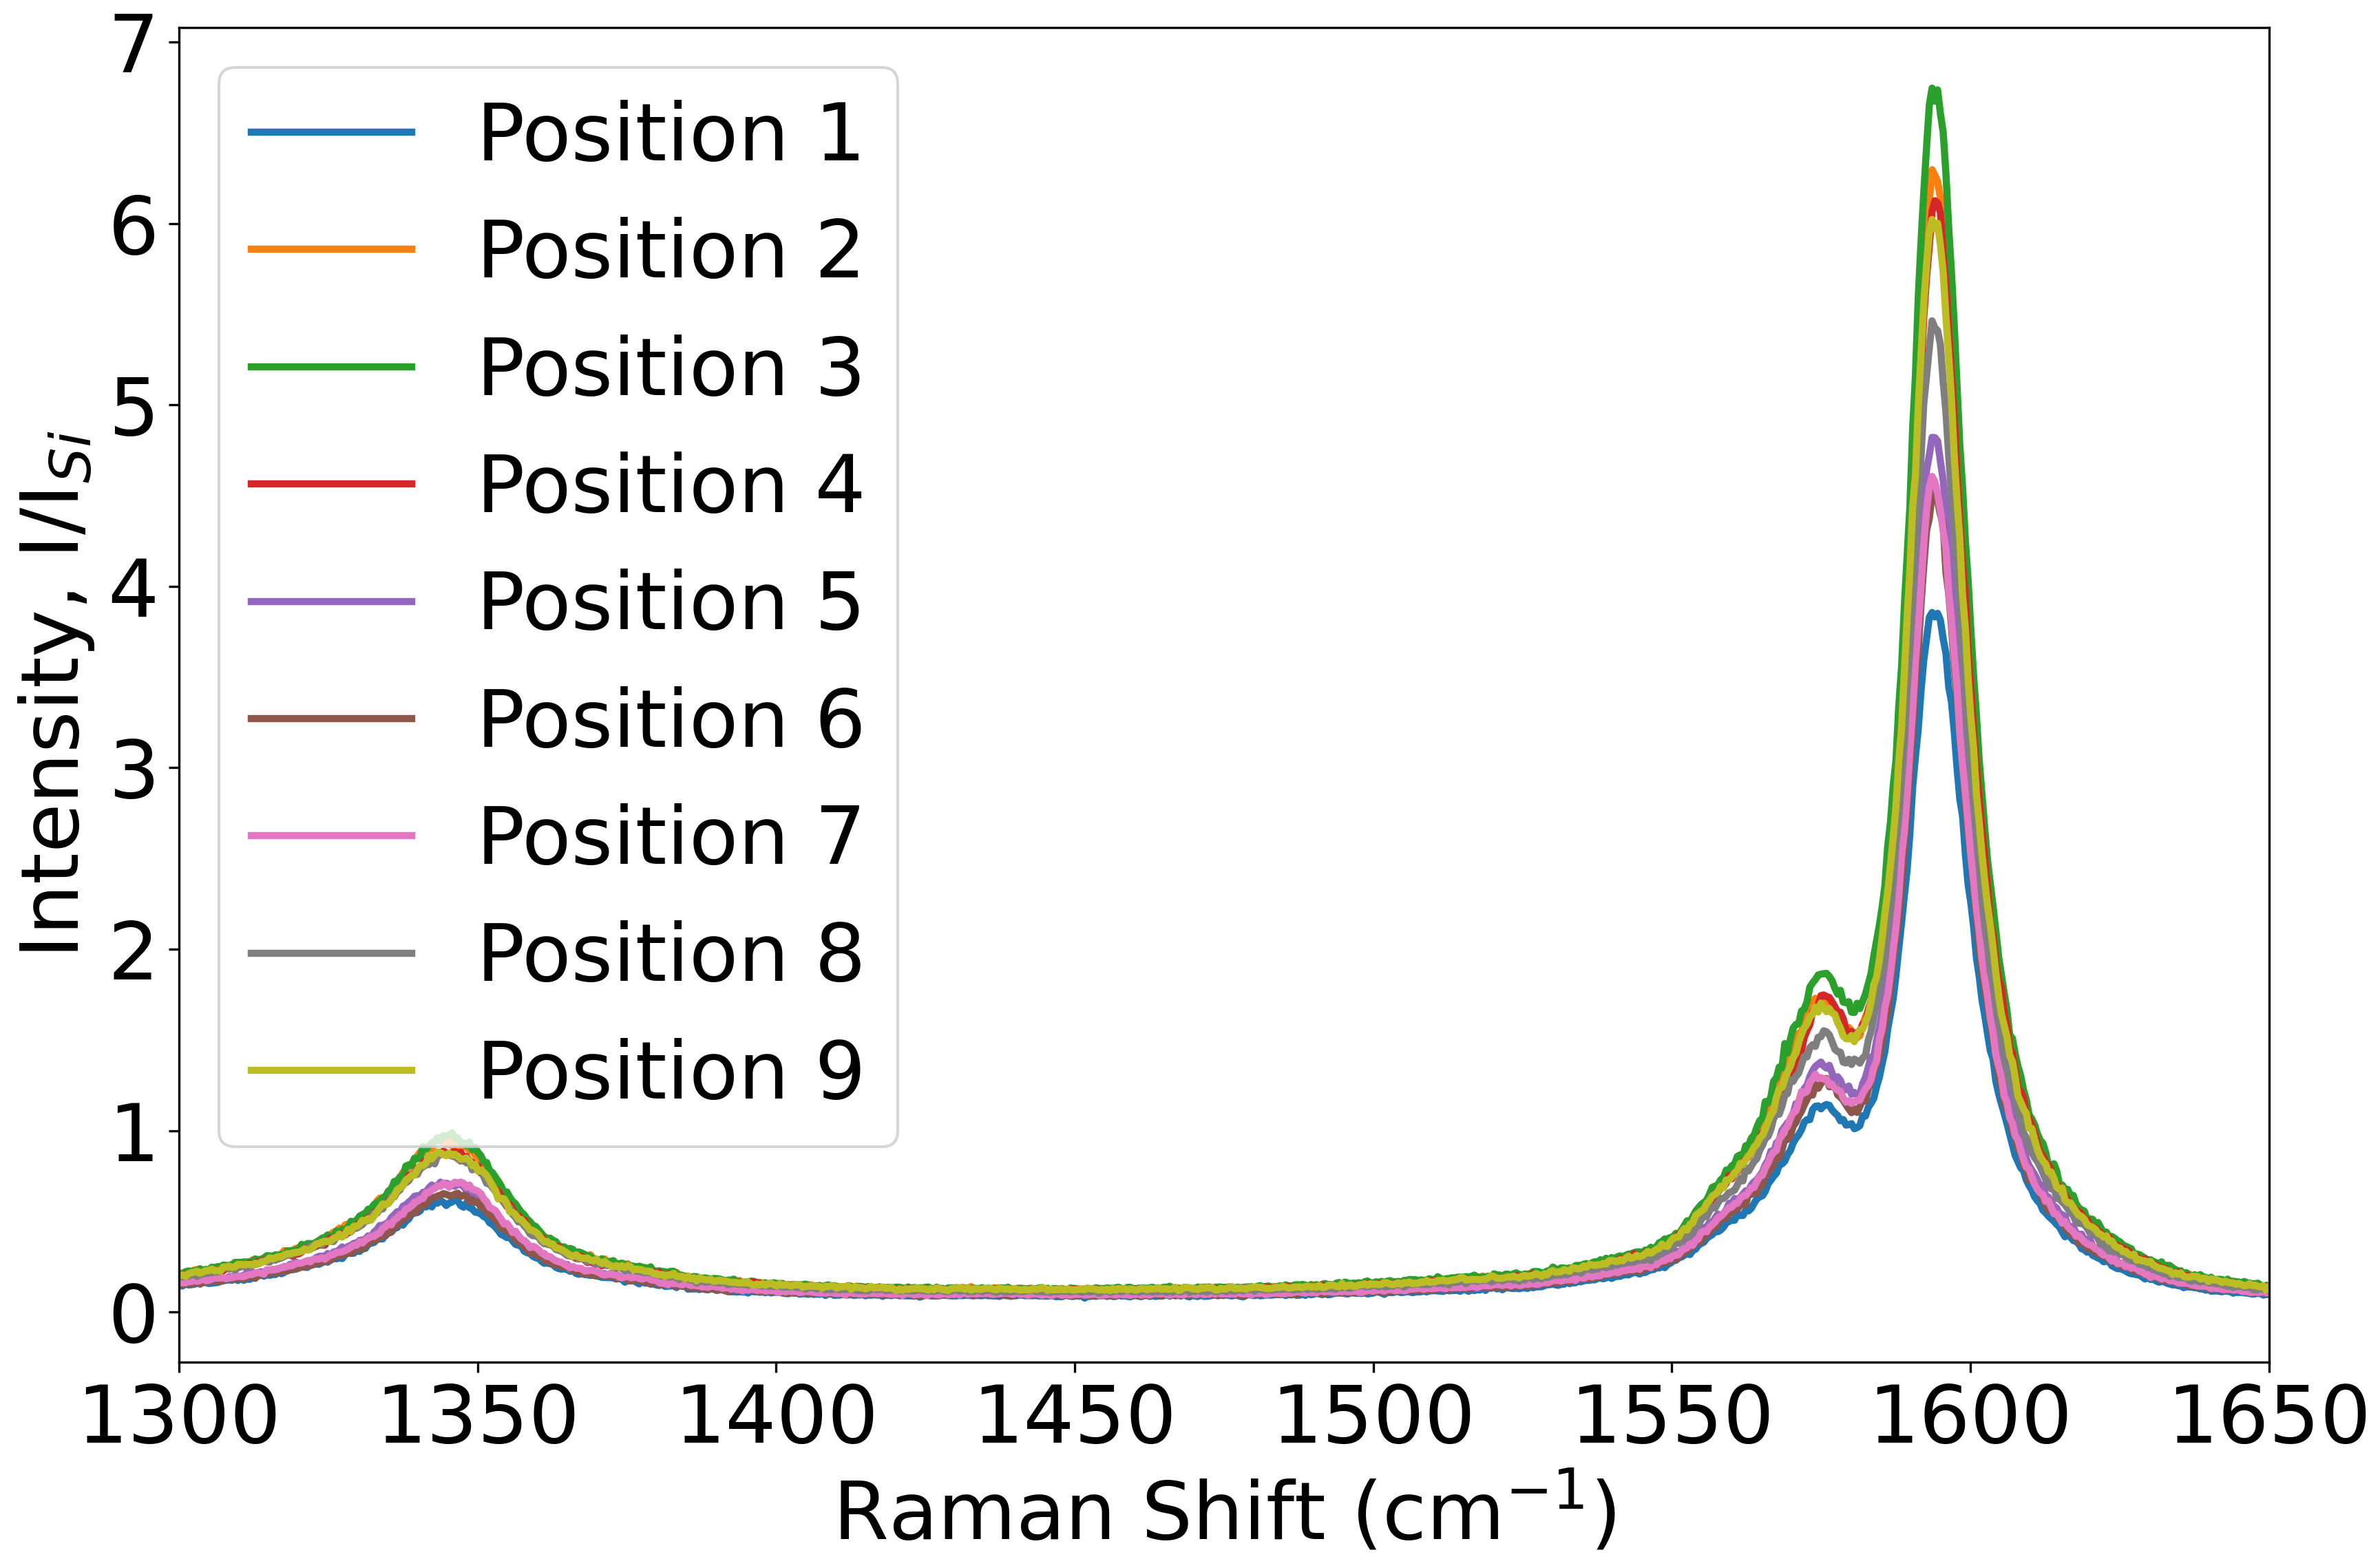
\includegraphics{figures/ch5/singletube_raman.png}

}

}

\subcaption{\label{fig-surfactant-deposited}}
\end{minipage}%
\newline
\begin{minipage}[t]{0.33\linewidth}

{\centering 

~

}

\end{minipage}%
%
\begin{minipage}[t]{0.35\linewidth}

{\centering 

\raisebox{-\height}{

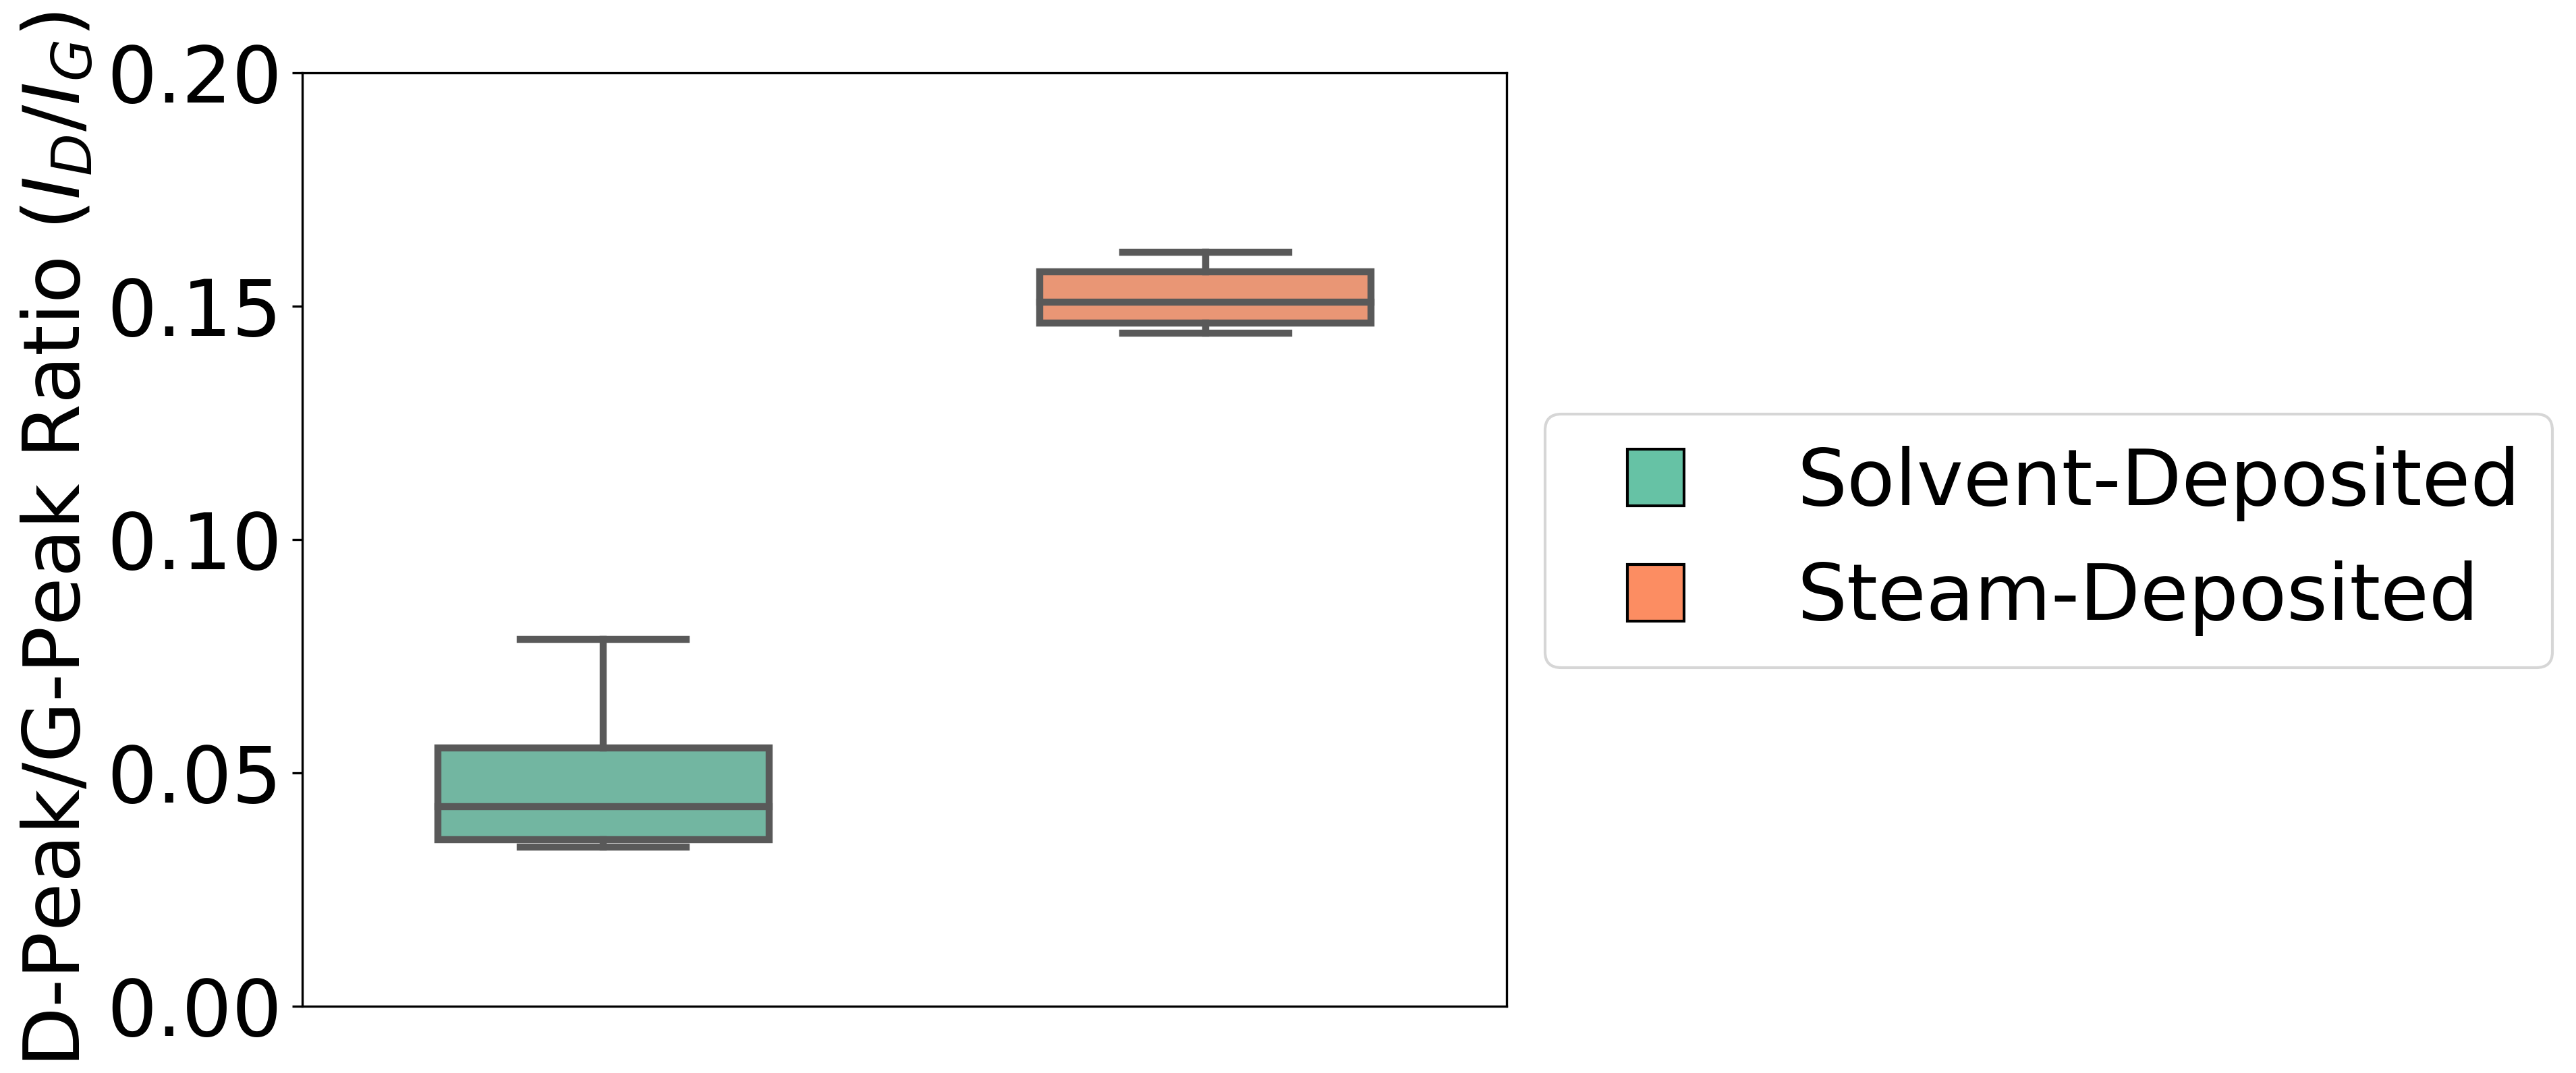
\includegraphics{figures/ch5/comparison-raman.png}

}

}

\subcaption{\label{fig-dg-peak-comparison}}
\end{minipage}%
%
\begin{minipage}[t]{0.33\linewidth}

{\centering 

~

}

\end{minipage}%

\caption{\label{fig-pristine-raman}A series of nine Raman spectra at
different locations across a 10 \(\mu\)m \(\times\) 50 \(\mu\)m carbon
nanotube film region, spaced at least 10 \(\mu\)m apart, with (a)
showing spectra from a film deposited in solvent and (b) showing spectra
from a film deposited in surfactant with steam present. (c) shows the
spread of the D-peak/G\(^+\)-peak spectral ratios corresponding to each
film.}

\end{figure}

Raman spectroscopy was also used to analyse and compare the deposited
carbon nanotube networks. Raman spectra were collected from a
solvent-deposited carbon nanotube film and a steam-assisted
surfactant-deposited film, both on silicon dioxide, in the manner
described in Section~\ref{sec-raman-characterisation}. These spectra
were then processed using the Python script mentioned in
Section~\ref{sec-raman-analysis}. For each location, spectra over two
wavenumber ranges were collected. A peak corresponding to the silicon
dioxide substrate, found in the range between 100 cm\(^{-1}\) and 650
cm\(^{-1}\), was used as a reference peak for the normalisation of
intensities across the range between 1300 cm\(^{-1}\) and 1650
cm\(^{-1}\). These normalised spectra are shown in
Figure~\ref{fig-pristine-raman}. In all spectra, a D-band comprising a
single D-peak is observed at \(\sim\) 1320 cm\(^{-1}\), and a G-band
comprising two G-peaks, G\(^-\) and G\(^+\) is observed between \(\sim\)
1525 cm\(^{-1}\) and \(\sim\) 1650 cm\(^{-1}\). These features are
characteristic of networks of semiconducting carbon nanotubes
\autocite{Dresselhaus2005,King2014}.

Closer inspection of the D peak and G peaks can give us important
information about network composition. G\(^-\) is a minor peak found at
\(\sim\) 1570 cm\(^{-1}\), while G\(^+\) is a larger feature at \(\sim\)
1590 cm\(^{-1}\). The G\(^+\) feature describes the in-plane vibration
of carbon bonds along the length of the carbon nanotubes, while the
G\(^-\) feature describes the in-plane vibration of bonds about the
nanotube circumference \autocite{King2014,Swiniarski2021}. The splitting
between the wavenumber location of the G\(^-\) and G\(^+\) local maxima
is lower in Figure~\ref{fig-surfactant-deposited} than in
Figure~\ref{fig-solvent-deposited}, indicating more metallic nanotubes
are present in the surfactant-deposited network
\autocite{Swiniarski2021}. The D-peak gives an indication of the defects
present in the carbon nanotube atomic structure
\autocite{King2014,Swiniarski2021}. We notice that the size of the
normalised D-peak is much lower in Figure~\ref{fig-solvent-deposited}
than in Figure~\ref{fig-surfactant-deposited}, indicating the solvent
deposition process introduces less defects to the carbon nanotubes than
surfactant-mediated deposition.

It is also possible to compare the relative magnitude of the D-peak and
G\(^+\)-peak intensity to quantify carbon nanotube structural disorder,
which disrupts in-plane lattice vibration
\autocite{Dresselhaus2005,King2014}. Figure~\ref{fig-dg-peak-comparison}
gives a summary of the ratios between the D-peak and G\(^+\)-peak across
all nine positions for the solvent-deposited and surfactant-deposited
film. It is immediately observed that I\(_{D}\)/I\(_{G}\) is
significantly larger for the steam-assisted, surfactant-deposited films
than for the solvent-deposited films. This is a further indication of
the presence of defects across the steam-deposited network. These
defects are likely introduced through the introduction of charge
impurites by surfactant aggregates present around the carbon nanotubes
\autocite{Christensen2022}. However, we also notice that the range of
values for the I\(_{D}\)/I\(_{G}\) ratio is lower for the
steam-deposited network. This spatially homogeneous vibrational
behaviour implies the steam-deposited network is more evenly distributed
than the solvent-deposited network, which matches the discussion in
Section~\ref{sec-pristine-morphology}.

\hypertarget{sec-pristine-electrical-characterisation}{%
\section{Electrical Characteristics of Pristine
Devices}\label{sec-pristine-electrical-characterisation}}

\hypertarget{carbon-nanotube-network-devices}{%
\subsection{Carbon Nanotube Network
Devices}\label{carbon-nanotube-network-devices}}

\begin{figure}

\begin{minipage}[t]{0.49\linewidth}

{\centering 

\raisebox{-\height}{

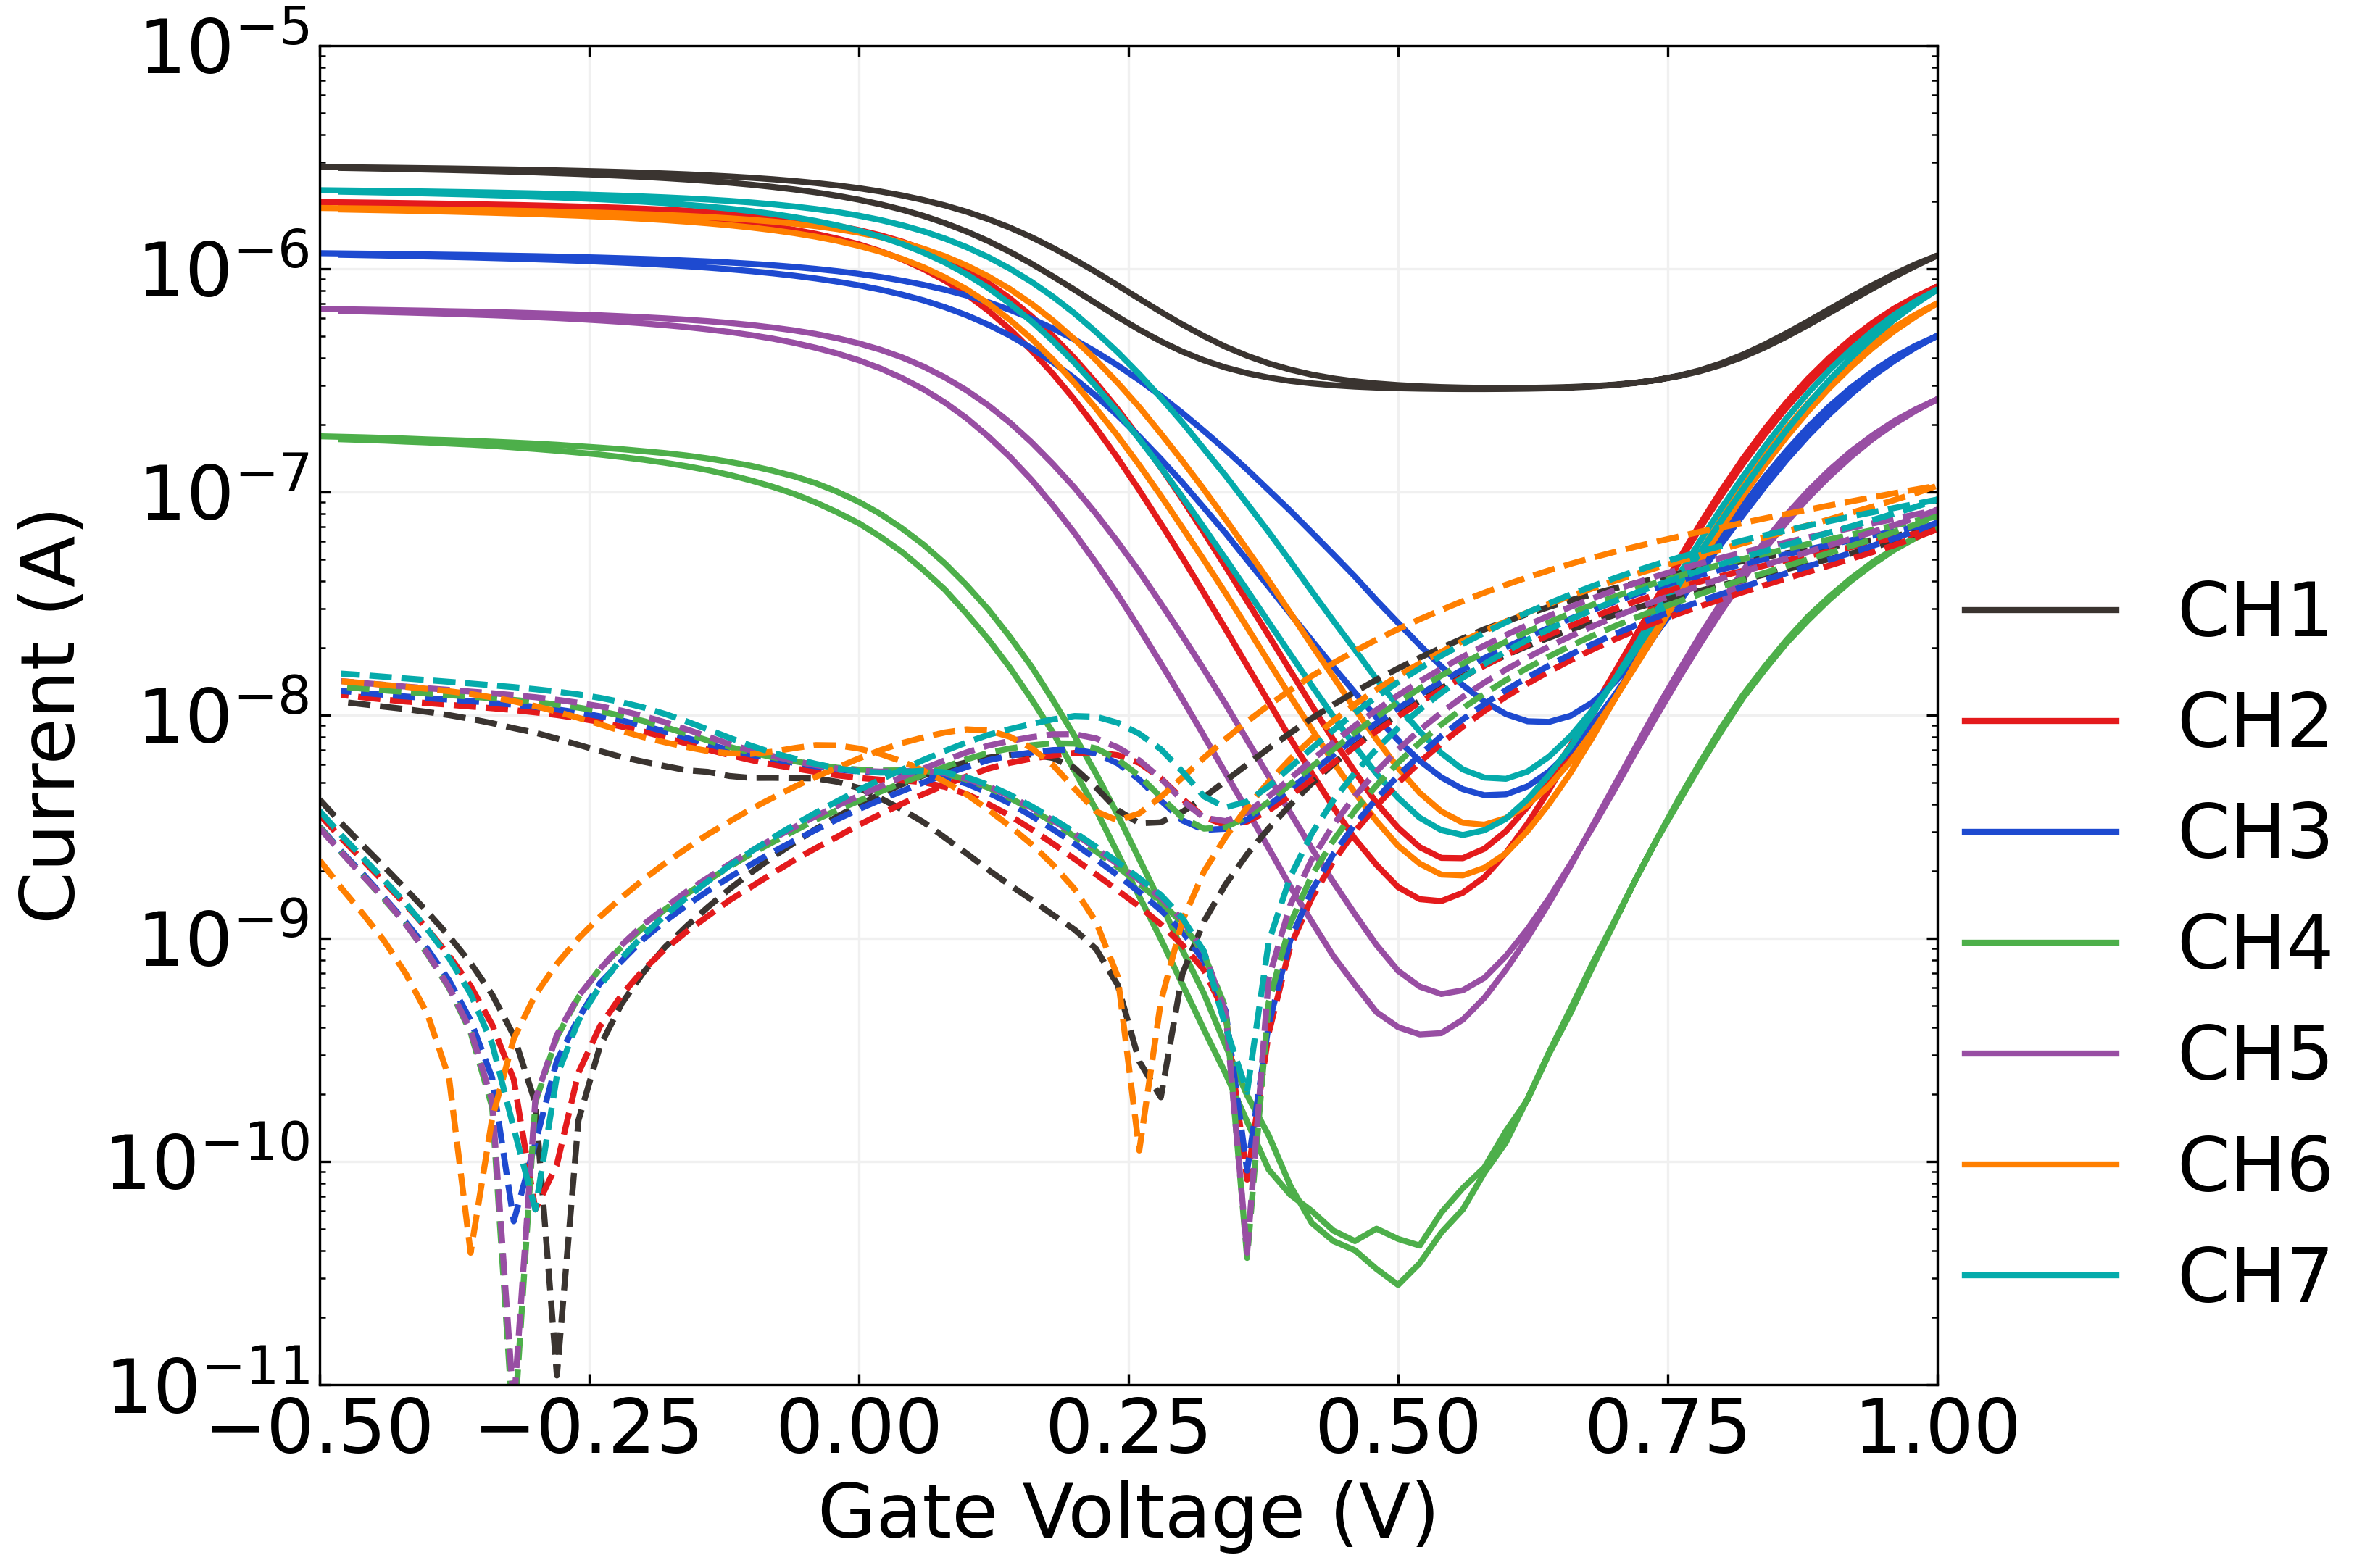
\includegraphics{figures/ch5/NTQ24C8_pristine_TXLG01_220211_solvent_gate.png}

}

}

\subcaption{\label{fig-solvent-tx-lg}}
\end{minipage}%
%
\begin{minipage}[t]{0.02\linewidth}

{\centering 

~

}

\end{minipage}%
%
\begin{minipage}[t]{0.49\linewidth}

{\centering 

\raisebox{-\height}{

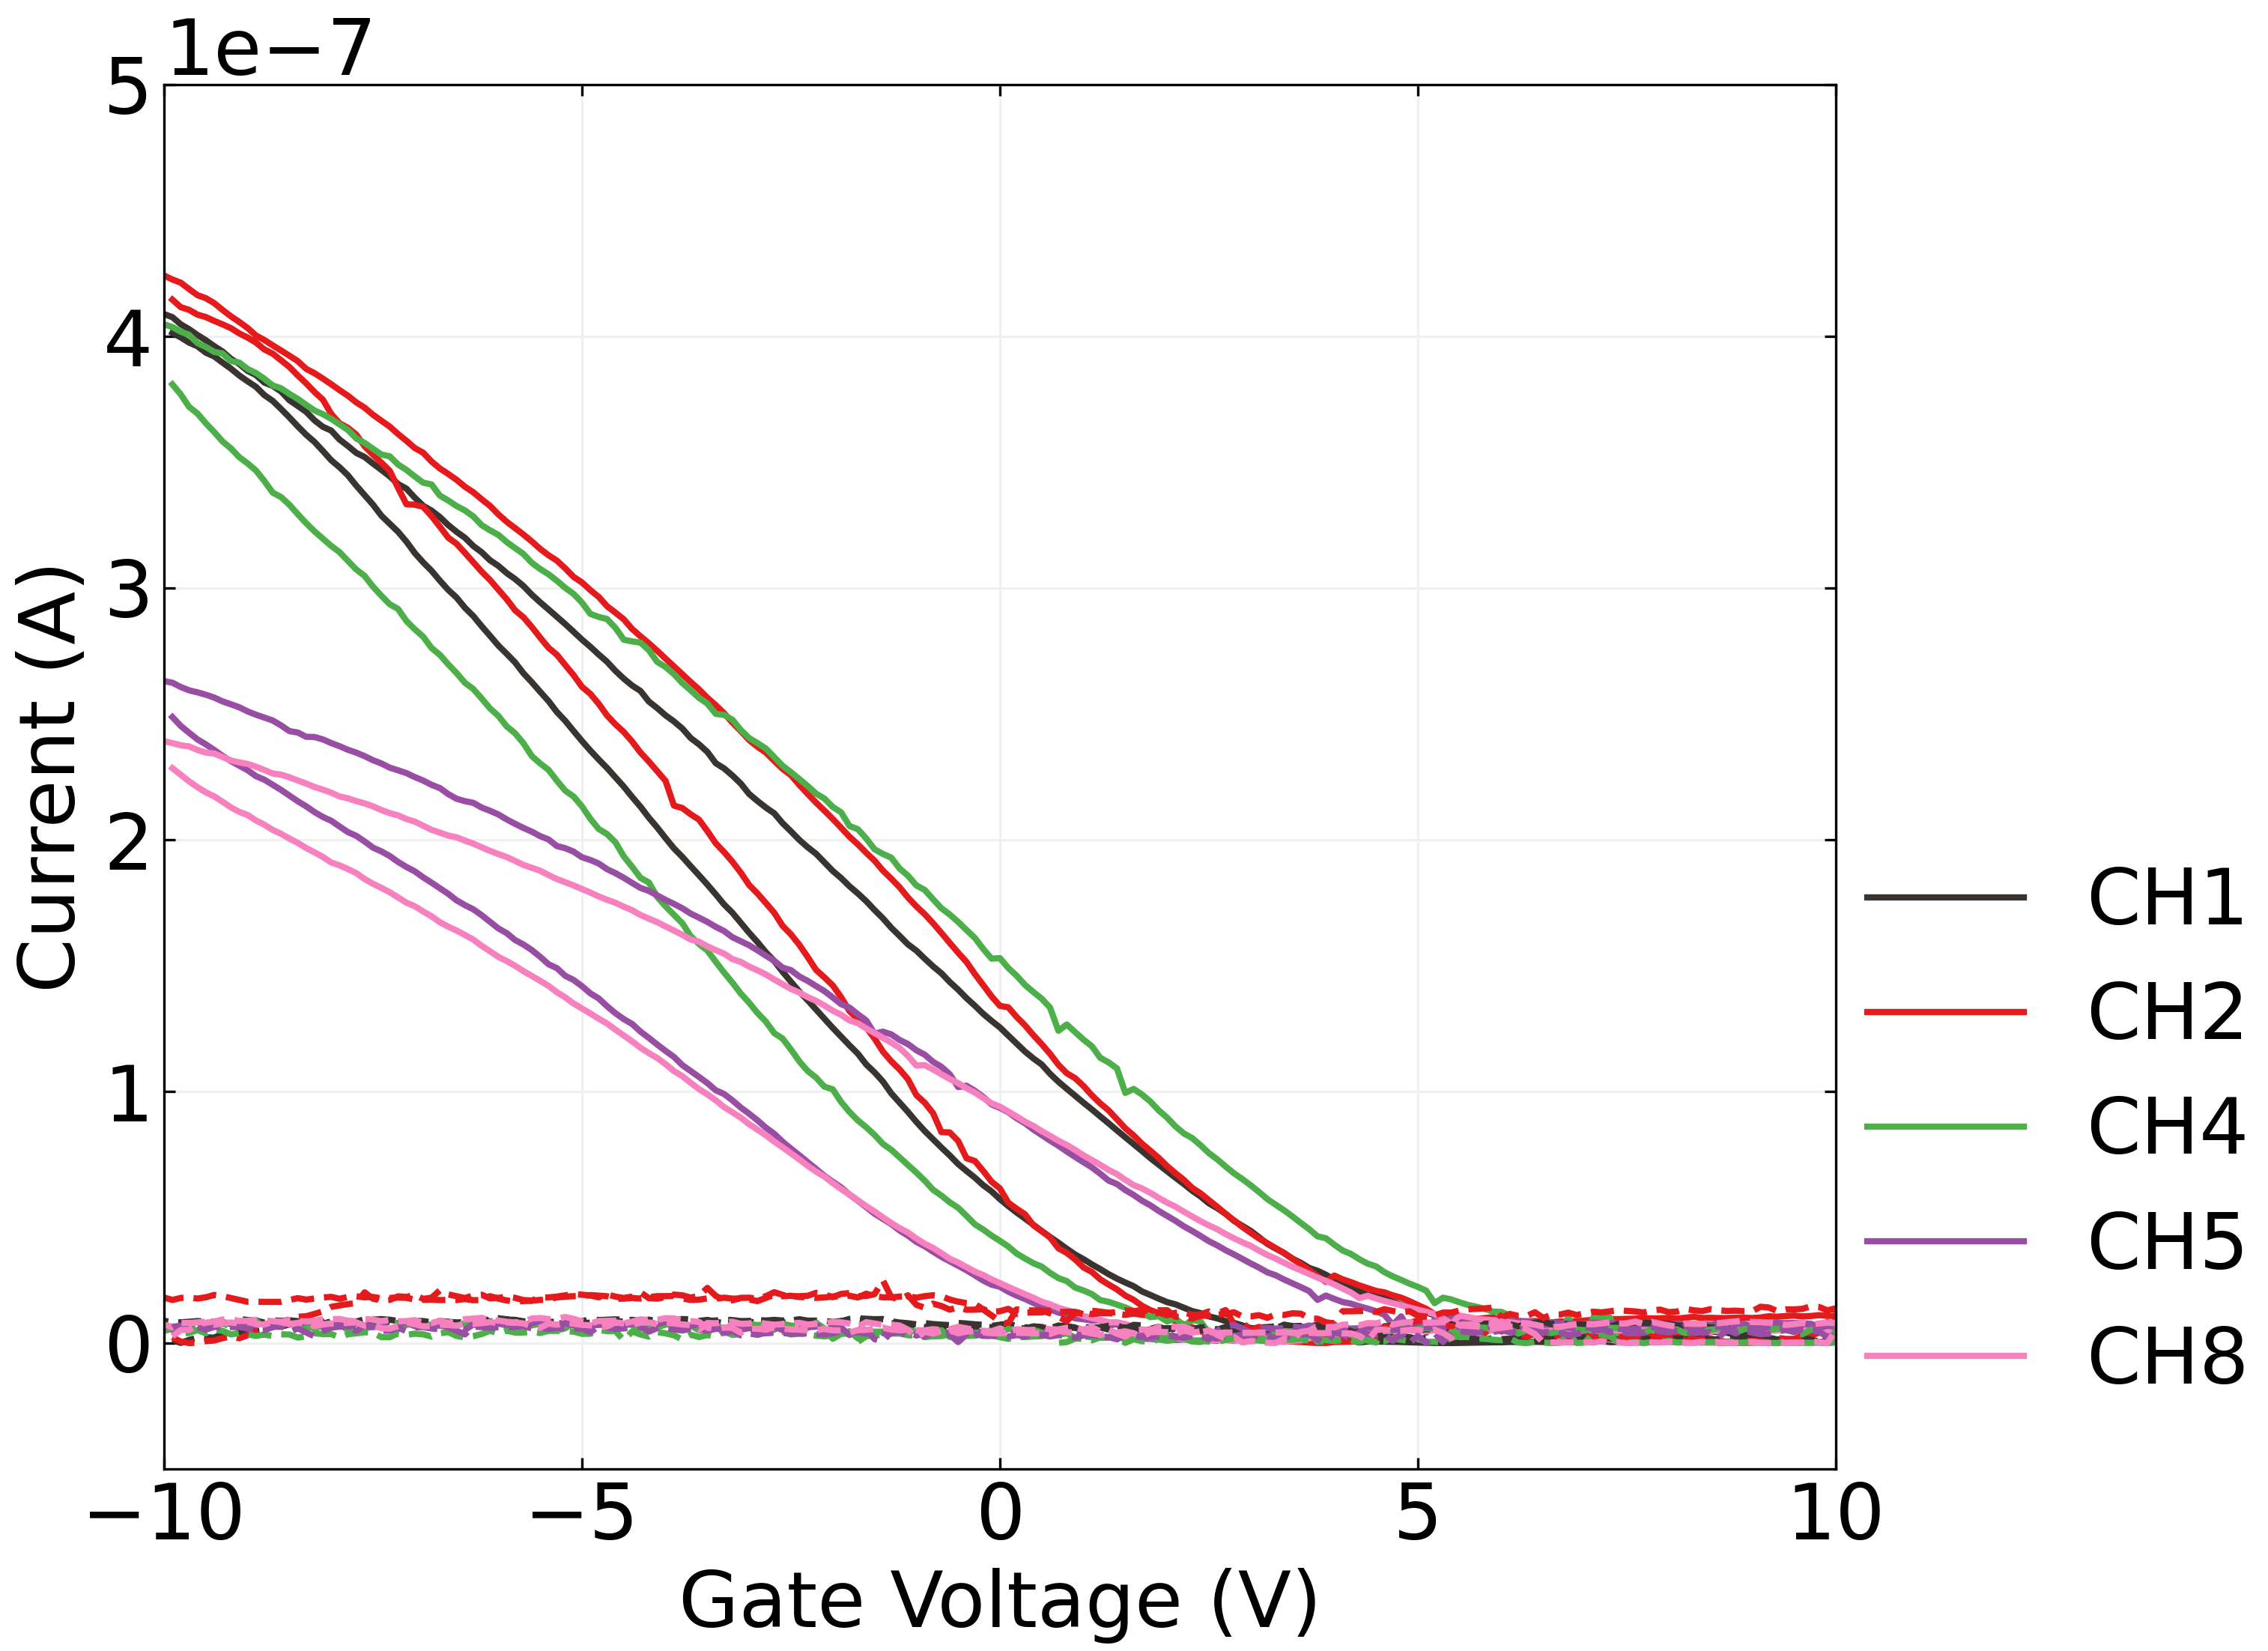
\includegraphics{figures/ch5/NTQ22C2_solvent_backgate.png}

}

}

\subcaption{\label{fig-solvent-tx-bg}}
\end{minipage}%
\newline
\begin{minipage}[t]{0.49\linewidth}

{\centering 

\raisebox{-\height}{

\includegraphics{figures/ch5/NTQ5C3_pristine_TXLG01_210602_nosteam_gate.png}

}

}

\subcaption{\label{fig-surf-tx-lg}}
\end{minipage}%
%
\begin{minipage}[t]{0.02\linewidth}

{\centering 

~

}

\end{minipage}%
%
\begin{minipage}[t]{0.49\linewidth}

{\centering 

\raisebox{-\height}{

\includegraphics{figures/ch5/Q5C10_nosteam_backgate.png}

}

}

\subcaption{\label{fig-surf-tx-bg}}
\end{minipage}%
\newline
\begin{minipage}[t]{0.49\linewidth}

{\centering 

\raisebox{-\height}{

\includegraphics{figures/ch5/NTQ31C6_pristine_TXLG01_230330_steam_gate.png}

}

}

\subcaption{\label{fig-steam-tx-lg}}
\end{minipage}%
%
\begin{minipage}[t]{0.02\linewidth}

{\centering 

~

}

\end{minipage}%
%
\begin{minipage}[t]{0.49\linewidth}

{\centering 

\raisebox{-\height}{

\includegraphics{figures/ch5/Q18C6_steam_backgate.png}

}

}

\subcaption{\label{fig-steam-tx-bg}}
\end{minipage}%

\caption{\label{fig-pristine-cnt-characteristics}Liquid-gated (left) and
back-gated (right) transfer characteristics of AZ\(^\circledR\) 1518
encapsulated field-effect transistors, where the film was deposited with
solvent in (a) and (b), deposited with surfactant in (c) and (d), and
deposited with surfactant in the presence of steam in (e) and (f). A
step size of 100 mV was used for the backgated sweeps in (a), (c) and
(e), while a step size of 20 mV was used for the liquid-gated sweeps in
(b), (d) and (f). Gate current (leakage current) is shown with a dashed
line. The source-drain voltage used for all sweeps was
\(V_{ds} = 100 \textrm{mV}\), and 1XPBS was used as the buffer for the
liquid-gated measurements here.}

\end{figure}

Each carbon nanotube device fabricated was electrically characterised as
described in Section~\ref{sec-electrical-characterisation}, and
electrical data was analysed using the Python code discussed in
Section~\ref{sec-field-effect-transistor-analysis}. Devices with a 100
nm or 300 nm SiO\(_2\) layer were used for liquid gated measurements,
and devices with a 100 nm SiO\(_2\) layer were used for backgated
measurements. Figure~\ref{fig-pristine-cnt-characteristics} displays
multi-channel measurements of representative devices fabricated as
described in Chapter~\ref{sec-fabrication}. To ensure a consistent
comparison, each device here was encapsulated with AZ\(^\circledR\) 1518
encapsulation before measurements were taken. The channels which did not
exhibit reliable transistor characteristics are not shown. These
`non-working' channels were either shorted, due to metal remaining on
the channel after lift-off, or were very low current, due to a very
sparse carbon nanotube network. Devices shown here with a
solvent-deposited carbon nanotube network were fabricated prior to Jan
2022; devices with a surfactant-deposited network without steam present
were fabricated prior to Jun 2021; devices with a surfactant-deposited
network without steam were fabricated prior to Sep 2022.

\begin{figure}

\begin{minipage}[t]{0.47\linewidth}

{\centering 

\raisebox{-\height}{

\includegraphics{figures/ch5/onoff_CNT.png}

}

}

\subcaption{\label{fig-on-off-ratio}}
\end{minipage}%
%
\begin{minipage}[t]{0.05\linewidth}

{\centering 

~

}

\end{minipage}%
%
\begin{minipage}[t]{0.47\linewidth}

{\centering 

\raisebox{-\height}{

\includegraphics{figures/ch5/SS.png}

}

}

\subcaption{\label{fig-subthreshold-slope}}
\end{minipage}%
\newline
\begin{minipage}[t]{0.26\linewidth}

{\centering 

~

}

\end{minipage}%
%
\begin{minipage}[t]{0.47\linewidth}

{\centering 

\raisebox{-\height}{

\includegraphics{figures/ch5/threshold_V.png}

}

}

\subcaption{\label{fig-threshold-voltage}}
\end{minipage}%
%
\begin{minipage}[t]{0.26\linewidth}

{\centering 

~

}

\end{minipage}%

\caption{\label{fig-sweep-parameters}These boxplots illustrate the
statistical distribution of (a) the on-off ratio, (b) the subthreshold
slope, and (c) the threshold voltage of AZ\(^\circledR\) 1518
encapsulated liquid-gated transistor channels corresponding to each type
of carbon nanotube film deposition. For each deposition type, electrical
characteristics were taken of 21 channels of at least three separate
devices. The boxes indicate the 25th and 75th percentile of the
distribution.}

\end{figure}

\hypertarget{liquid-gated-cntfets}{%
\subsubsection*{Liquid-Gated CNTFETs}\label{liquid-gated-cntfets}}
\addcontentsline{toc}{subsubsection}{Liquid-Gated CNTFETs}

The liquid-gated devices in Figure~\ref{fig-solvent-tx-lg},
Figure~\ref{fig-surf-tx-lg} and Figure~\ref{fig-steam-tx-lg} each
exhibited ambipolar characteristics, commonly observed in liquid-gated
carbon nanotube network FETs
\autocite{Kauffman2008,Heller2009,JongYu2009,Derenskyi2014,Murugathas2018,Albarghouthi2022}.
When devices were appropriately configured, leakage current (shown by
the dashed traces) did not exceed \(\sim 1 \times 10^{-7}\) V across the
forward and reverse sweep. The devices shown which used steam-deposited
carbon nanotube films showed the least hysteresis. From
Section~\ref{sec-pristine-AFM}, we know the mean diameter of the bundles
in these films is about 0.9 nm less than the mean bundles in films
deposited without steam present, and 5.5 nm less than those in films
deposited in solvent. Hysteresis is known to scale roughly linearly with
bundle diameter, due to trapped charge increasing as bundle density of
states is increased \autocite{Pop2009}. Steam-deposited devices also
showed significantly less channel-to-channel variation in electrical
characteristics more generally. Channel 1 in
Figure~\ref{fig-solvent-tx-lg} has a much higher off-current than the
other channels of the same device, which appears to be due to a
uncommonly high proportion of metallic carbon nanotubes present in the
network conduction pathways of this channel
\autocite{Rouhi2011,Zaumseil2015}.

A summary of key parameters of pristine liquid-gated devices is shown in
Figure~\ref{fig-sweep-parameters}. The full dataset consists of three
sets of 21 liquid-gated transfer characteristics of working channels,
with each set corresponding to the use of a particular method of carbon
nanotube network deposition in the device fabrication. Measurements from
at least three devices are included in each set. Each entry in the
summary corresponds to the average of the specific parameter in the
forward and reverse sweep direction. When steam was used for surfactant
deposition of films, the resulting devices showed highly consistent
channel-to-channel electrical properties. As the carbon nanotube films
on these devices are relatively dense, as seen in
Figure~\ref{fig-steaming-network}, we know that the network is well
above the percolation threshold. As many carbon nanotube pathways
connect across the channel in parallel, small variations in the network
morphology have less of an impact on the overall channel behaviour
\autocite{Murugathas2018}.We also see from
Figure~\ref{fig-cnt-histogram} and Table~\ref{tbl-histogram-parameters}
that the range of bundle sizes is relatively low in the steam-deposited
films used in these devices, meaning the electrical behaviour of
dominant conduction pathways is more spatially consistent. The
repeatable subthreshold regime behaviour between channels seen for
steam-deposited devices is a desirable attribute for reliable real-time
multiplexed biosensing \autocite{Kauffman2008,Heller2009,Gao2010}.

Channels from surfactant-deposited film devices usually showed a larger
on-off ratio and subthreshold slope than those from solvent-deposited
devices. Decreasing the ratio of gate-sensitive semiconducting carbon
nanotubes to metallic nanotubes tends to decrease the on-off ratio
\autocite{LeMieux2008,Rouhi2011,Zaumseil2015,Murugathas2018}.
Section~\ref{sec-pristine-raman} seems to indicate there are more
metallic nanotubes present in the surfactant-deposited films than in the
solvent-deposited films. However, percolating conduction pathways
dominate device behaviour and nanotube pathways across the channel with
a lower degree of bundling are less likely to contain metallic tubes
\autocite{Murugathas2018}. Therefore, the larger on-off ratio for
surfactant-deposited film devices is likely a result of their reduced
nanotube bundle size and reduced bundle size variation relative to other
films, as discussed in Section~\ref{sec-pristine-morphology}. The larger
subthreshold slope is likely due to increased mobility from a denser
nanotube network in surfactant-deposited films \autocite{Rouhi2011}, as
seen in Figure~\ref{fig-steaming-network}. A larger on-off ratio and
subthreshold slope results in a larger change in conductance in response
to changes in the transfer characteristic curve. Therefore, the larger
on-off ratio and subthreshold slope of steam-deposited devices is
desirable for improved sensor performance
\autocite{Kauffman2008,Heller2009,Gao2010}.

All channels characterised had a positive threshold voltage
(\(V_{th}\)). The threshold voltage was largest and most consistent for
steam-assisted surfactant-deposited films. The relatively high values of
\(V_{th}\) which correspond to channel measurements from steam-assisted
surfactant-deposited devices indicates increased \(p\)-doping of the
network relative to networks deposited via alternative processes
\autocite{Kang2005,Heller2008,Murugathas2018}. As seen from
Figure~\ref{fig-steamed-surfactant}-f and
Figure~\ref{fig-dg-peak-comparison}, the steam deposition process leads
to the presence of significant, persistent surfactant aggregates. It has
been previously established that residual surfactant can \(p\)-dope
carbon nanotubes, alongside enhancing \(p\)-doping from adsorped oxygen
and water \autocite{Kane2014,Nonoguchi2018,Christensen2022}. The
presence of residual surfactant may also explain the lowered
subthreshold slope, and therefore mobility, of the steam-deposited
devices relative to devices with films deposited in surfactant without
steam. The analysis by Kane \emph{et al.} shows that the thermal
annealling at 150\(^\circ\)C used in this work to remove residual
surfactant is likely inadequate for this purpose. Oxidation of devices
and vacuum annealling at high temperatures (\textgreater{}
600\^{}\circ\$C) may be required for effective desorption o f the
persistent surfactant \autocite{Kane2014,Barnett2018}. Devices using
films made using the alternative two methods have the advantage of not
requiring careful treatment to remove surfactant.

\hypertarget{back-gated-cntfets}{%
\subsubsection*{Back-Gated CNTFETs}\label{back-gated-cntfets}}
\addcontentsline{toc}{subsubsection}{Back-Gated CNTFETs}

When characterising devices using the vapour delivery system chip
carrier, the setup arrangement meant all measurements were taken using a
backgate. From Figure~\ref{fig-solvent-tx-bg},
Figure~\ref{fig-surf-tx-bg} and Figure~\ref{fig-steam-tx-bg}, we see
backgated devices exhibited \emph{p}-type transistor behaviour. Gate
current leakage was negligible, as shown by the dashed line staying
close to zero across the sweep. Significant hysteresis was observed. The
hysteresis can be explained by the presence of defects or charge traps
within and on the surface of the silicon dioxide and at interfaces
between the silicon dioxide and carbon nanotubes
\autocite{Lee2007,Lee2012,Ha2014}. The hysteresis observed was much
greater than for the corresponding liquid-gated sweeps on the right. The
devices fabricated with a solvent-based deposition were switched off at
a lower voltage than the devices which used surfactant during
deposition.

\begin{figure}

\begin{minipage}[t]{0.47\linewidth}

{\centering 

\raisebox{-\height}{

\includegraphics{figures/ch5/Q35C3_nobuffer.png}

}

}

\subcaption{\label{fig-no-buffer}}
\end{minipage}%
%
\begin{minipage}[t]{0.05\linewidth}

{\centering 

~

}

\end{minipage}%
%
\begin{minipage}[t]{0.47\linewidth}

{\centering 

\raisebox{-\height}{

\includegraphics{figures/ch5/Q35C3_buffer.png}

}

}

\subcaption{\label{fig-50uL-buffer}}
\end{minipage}%

\caption{\label{fig-buffer-effect-on-backgate}Backgated transfer sweeps
were taken of an single unencapsulated device with a 300 nm SiO\(_2\)
layer and steam assisted surfactant-deposited carbon nanotube network
channels before and after being covered in \(50 \mu\)L 1XPBS
electrolyte.}

\end{figure}

Transfer measurements were taken to determine whether backgated
measurements could be taken of an unencapsulated device in the vapour
sensor chamber with 1XPBS covering the channels.
Figure~\ref{fig-buffer-effect-on-backgate} shows the behaviour of an
unencapsulated backgated device with a 300 nm SiO\(_2\) layer before and
after being covered by 50 \(\mu\)L of 1XPBS (phosphate buffered saline).
The on-off ratio and hysteresis of the channels increase significantly.
The presence of water increases hysteresis through introducing charge
traps at the silicon dioxide surface around the carbon nanotubes and at
the surface of the nanotubes themselves
\autocite{Kim2003,Lee2007,Franklin2012,Ha2014}. There is also a
significant increase in current leakage to the backgate for larger
applied voltages, despite the electrolyte having no visible physical
contact with the silicon backgate or copper plane. This leakage current
may simply be due to an increase in relative humidity around the device
due to the presence of water \autocite{Conseil2014}. As any variation in
threshold voltage due to hysteresis and significant leakage current are
undesirable for sensing procedures, this configuration was not used for
vapour sensing purposes.

\hypertarget{graphene-devices}{%
\subsection{Graphene Devices}\label{graphene-devices}}

\begin{figure}

\begin{minipage}[t]{0.47\linewidth}

{\centering 

\raisebox{-\height}{

\includegraphics{figures/ch5/JG098_pristine_TXLG01_5mVstep_220920_norinse.png}

}

}

\subcaption{\label{fig-graphene-transfer-1}}
\end{minipage}%
%
\begin{minipage}[t]{0.05\linewidth}

{\centering 

~

}

\end{minipage}%
%
\begin{minipage}[t]{0.47\linewidth}

{\centering 

\raisebox{-\height}{

\includegraphics{figures/ch5/JGQ00D6_pristine_TXLG01_5mVstep_220914_norinse.png}

}

}

\subcaption{\label{fig-graphene-transfer-2}}
\end{minipage}%
\newline
\begin{minipage}[t]{0.47\linewidth}

{\centering 

\raisebox{-\height}{

\includegraphics{figures/ch5/JG098_ch1_absolute_values_with_gate_current.png}

}

}

\subcaption{\label{fig-graphene-transfer-comparison-1}}
\end{minipage}%
%
\begin{minipage}[t]{0.05\linewidth}

{\centering 

~

}

\end{minipage}%
%
\begin{minipage}[t]{0.47\linewidth}

{\centering 

\raisebox{-\height}{

\includegraphics{figures/ch5/JGQ00D6_ch3_absolute_values_with_gate_current.png}

}

}

\subcaption{\label{fig-graphene-transfer-comparison-2}}
\end{minipage}%

\caption{\label{fig-pristine-graphene}These figures show liquid-gated
transfer characteristics of channels from two AZ\(^\circledR\) 1518
encapsulated graphene devices. The characteristics of working device
channels upon initial exposure to 1XPBS are shown in (a) and (b). The
transfer characteristics of channel 1 in (a) and channel 5 in (b) after
various degrees of exposure to 1XPBS are shown in (c) and (d)
respectively, with each transfer sweep numbered in the order the sweeps
were taken. The dashed lines correspond to measurements of gate leakage
current.}

\end{figure}

Graphene field-effect transistor devices were electrically characterised
in the manner described in Section~\ref{sec-electrical-characterisation}
and analysed using the Python code discussed in
Section~\ref{sec-field-effect-transistor-analysis}.

Figure~\ref{fig-pristine-graphene} shows the liquid-gated transfer
characteristics of two graphene devices. These devices were fabricated
prior to Jun 2021. Both devices exhibit the ambipolar characteristics
typical of liquid-gated graphene devices
\autocite{Heller2009a,Heller2010,Xia2010,Kireev2017}. As with the carbon
nanotube network devices, leakage current remained below \(\sim\) 1
\(\times\) \(10^{-7}\) V across both the forward and reverse sweep.
Hysteresis between the forward and reverse sweep is caused by trapping
of charge within and on the surface of the SiO\(_{2}\) dielectric
\autocite{Bartolomeo2011}. The major Dirac point for these devices is
slightly to the right of V\(_{\textrm{Dirac}} \approxeq\) 0 V, which
indicates \(p\)-doping of the channel. This slight \(p\)-doping is
likely a result of a adsorption of oxygen and water from the air and
residue resist from photolithography
\autocite{Cheng2011,Shin2012,Kireev2017}.

Some devices exhibited a double-minima feature, indicating the presence
of two Dirac points. This effect arises due to doping of graphene by the
metal contacts. In shorter length channels, metal doping affects the
entire channel length, leading to a consistent Fermi level and a single
Dirac point. However, for longer channel lengths like ours, the doping
effect from metal contact no longer reaches the entire channel, leading
to a difference in Fermi level between the graphene in the channel and
graphene under the metal contact. The difference in Fermi levels results
in the presence of a second Dirac point
\autocite{Bartolomeo2011,Feng2014,Peng2018}. The global minimum of the
transfer characteristic can be referred to as the `major' Dirac point.

Figure~\ref{fig-pristine-graphene} also shows the effect of 1XPBS on the
graphene channels. The channels were measured on exposure to 1XPBS,
after exposure to 1XPBS for one hour, and after the device surface was
rinsed and 1XPBS was replaced in the well one time, two times and three
times successively. A slight negative shift of the major Dirac point was
observed. This effect is possibly a result of gate bias stress, where
successive transfer sweeps introduce charge traps to the graphene layer
and alters the current level at a given gate voltage
\autocite{Bargaoui2018,Noyce2019}. Alternatively, Kireev \emph{et al.}
found that a series of liquid-gated sweeps also reduced the size of the
second Dirac point, and suggested that it indicated the gate current was
removing atmospheric contaminants from the graphene surface via current
annealing \autocite{Kireev2017}. This could be explained as the removal
of contaminants causing improved contact between the metal and graphene
surface, and thus increasing metal doping and consistency of the Fermi
level across the channel. If the contaminants removed are \(p\)-dopants,
then this effect could also explain the negative shift of the major
Dirac point.

\hypertarget{tbl-graphene-parameters}{}
\begin{table}
\caption{\label{tbl-graphene-parameters}Average on-off ratio and major Dirac point voltage for AZ® 1518
encapsulated liquid-gated graphene transistor channels at various stages
of exposure to 1XPBS. Electrical characteristics were taken of 6
channels total, three channels from each of two devices. }\tabularnewline

\centering
\begin{tabular}{lccc}
\toprule
 & 1XPBS: Initial & 1XPBS: After 1 hr & 1XPBS: Rinse\\
\midrule
On-Off Ratio (arb.) & 5.1 ± 0.3 & 5.0 ± 0.7 & 5.0 ± 0.6\\
Dirac Point Voltage (V) & 0.28 ± 0.04 & 0.31 ± 0.03 & 0.28 ± 0.02\\
\bottomrule
\end{tabular}
\end{table}

Table~\ref{tbl-graphene-parameters} shows the on-off ratio and major
Dirac point voltage of the graphene devices. Apart from the
previously-mentioned slight negative shift of the major Dirac point,
these values were highly consistent before and after exposure to 1XPBS.

\hypertarget{sec-dummy-sensing}{%
\section{Real-Time Salt Concentration Sensing with Phosphate Buffered
Saline}\label{sec-dummy-sensing}}

\hypertarget{sec-baseline-drift}{%
\subsection{Control Series and Baseline
Drift}\label{sec-baseline-drift}}

\hypertarget{tbl-threshold-voltages}{}
\begin{longtable}[]{@{}lrrrrrr@{}}
\caption{\label{tbl-threshold-voltages}The threshold voltages \(V_{th}\)
of each working channel of a steam-deposited device, and the difference
between each \(V_{th}\) and the mean device threshold voltage
\(V_{th, mean}\).\\
}\tabularnewline
\toprule\noalign{}
Channels & CH1 & CH2 & CH3 & CH5 & CH6 & CH7 \\
\midrule\noalign{}
\endfirsthead
\toprule\noalign{}
Channels & CH1 & CH2 & CH3 & CH5 & CH6 & CH7 \\
\midrule\noalign{}
\endhead
\bottomrule\noalign{}
\endlastfoot
Threshold voltage (mV) & 160 & 150 & 130 & 140 & 180 & 140 \\
Relative to mean (mV) & 10 & 0 & -20 & -10 & 30 & -10 \\
\end{longtable}

To verify the sensitivity of the fabricated field-effect transistors and
therefore verify their suitability for sensing, control measurements
replicating a typical sensing experiment were taken before
functionalising the device channels. This involved first ensuring the
device showed no response to 1XPBS, a sequence referred to here as the
`PBS control series'. The PDMS well contained 80 \(\mu\)L 1X PBS at 0 s.
The PBS control series ran over the first 1800 s, with 20\(\mu\)L
phosphate buffer saline (1XPBS) additions at 100 s, 200 s and 300 s, and
20\(\mu\)L subtractions at 400 s, 500 s and 600 s. The device was left
untouched over the next 1200 s to allow the current level to settle. The
gate voltage was held at \(V_g\) = 0 V.

Figure~\ref{fig-transfer-sweeps} shows the transfer sweeps of the six
working channels of a steam-assisted surfactant-deposited carbon
nanotube field-effect transistor encapsulated with AZ\(^\circledR\)
1518, fabricated in Mar 2023 and measured using the PXIe. The central
`negative current' feature in the transfer characteristics of channels 1
and 7 is due to unphysical measurements which come from equipment error
and can be treated as zero current passing through the channel. The
threshold voltages of the channels are shown in
Table~\ref{tbl-threshold-voltages}. Table~\ref{tbl-threshold-voltages}
also shows the difference between the threshold voltage of each channel
and the mean threshold voltage of the device. The mean threshold voltage
was \(V_{th}\) = \(150 \pm 20\) mV. As discussed previously, the
electrical characteristics are highly consistent between the channels
due to the film deposition method used.

\begin{figure}

\begin{minipage}[t]{0.45\linewidth}

{\centering 

\raisebox{-\height}{

\includegraphics{figures/ch5/NTQ31C1_pristine_TXLG02_230322.png}

}

}

\subcaption{\label{fig-transfer-sweeps}}
\end{minipage}%
%
\begin{minipage}[t]{0.05\linewidth}

{\centering 

~

}

\end{minipage}%
%
\begin{minipage}[t]{0.50\linewidth}

{\centering 

\raisebox{-\height}{

\includegraphics{figures/ch5/NTQ31C1_pristine_saltconc_sample_230324_control.png}

}

}

\subcaption{\label{fig-linear-fit}}
\end{minipage}%
\newline
\begin{minipage}[t]{0.28\linewidth}

{\centering 

~

}

\end{minipage}%
%
\begin{minipage}[t]{0.45\linewidth}

{\centering 

\raisebox{-\height}{

\includegraphics{figures/ch5/NTQ31C1_pristine_saltconc_sample_230324_linear_fit_exp.png}

}

}

\subcaption{\label{fig-exp-fit}}
\end{minipage}%
%
\begin{minipage}[t]{0.28\linewidth}

{\centering 

~

}

\end{minipage}%

\caption{\label{fig-salt-conc-control-series}The transfer
characteristics in (a) were taken of the steam-deposited carbon nanotube
field-effect transistor used here for an example of salt concentration
sensing. The absolute values of measurements are shown, so that negative
values resulting from measurement error can be visualised. Linear fits
to the PBS control series from each channel from 1200 s onwards are
shown in (b), while exponential fits to the PBScontrol series from
\(0-1200\) with the linear fit subtracted are shown in (c). No
significant response to PBS additions are seen at any of the addition
times from 100 s - 600 s.}

\end{figure}

Figure~\ref{fig-linear-fit} shows the PBS control series corresponding
to each device channel alongside gate current. In both series, there is
no clear stepwise response to any addition or subtraction of 1XPBS. Gate
leakage current remains negligible across the entire control series,
with no change in response to 1XPBS additions. We see that the current
has a period of faster decay followed by slower baseline drift, similar
to observations by Lin \emph{et al.} and more recently Noyce \emph{et
al.} for parallel arrangements of single carbon nanotubes in air or
vacuum \autocite{Lin2006,Noyce2019}. This effect results from changes in
the occupancy of charge traps in and around the substrate and carbon
nanotubes. The magnitude of baseline drift is lower for our devices than
for those characterised by Noyce \emph{et al.}, which may be a result of
numerous device and setup differences which affect the presence of
charge traps. These differences include liquid-gating instead of
back-gated, the use of a network of carbon nanotubes instead of single
nanotubes, a different channel length, the use of a 300 nm instead of 90
nm SiO\(_2\) layer, and the use of an asymmetric, liquid-gated transfer
sweep over a shorter voltage range to characterise devices before each
control series was measured \autocite{Noyce2019}.

\hypertarget{tbl-linear-fits}{}
\begin{longtable}[]{@{}lllllll@{}}
\caption{\label{tbl-linear-fits}The coefficients of linear fits to the
PBS control series of each channel between \(1200-1800\) s, where \(m\)
is the gradient and \(b\) is the constant term.\\
}\tabularnewline
\toprule\noalign{}
Channels & CH1 & CH2 & CH3 & CH5 & CH6 & CH7 \\
\midrule\noalign{}
\endfirsthead
\toprule\noalign{}
Channels & CH1 & CH2 & CH3 & CH5 & CH6 & CH7 \\
\midrule\noalign{}
\endhead
\bottomrule\noalign{}
\endlastfoot
\(m\) (pA/s) & -5.1±0.2 & -7.2±0.1 & -6.5±0.1 & -5.0±0.1 & -7.6±0.1 &
-5.1±0.2 \\
\(b\) (\(\mu\)A) & 0.316 & 0.316 & 0.308 & 0.218 & 0.364 & 0.332 \\
\end{longtable}

\hypertarget{tbl-exp-fits}{}
\begin{longtable}[]{@{}llllll@{}}
\caption{\label{tbl-exp-fits}The coefficients of exponential fits to the
PBS control series of each channel between \(0-1200\) s, after the
linear fit has been subtracted, where \(a\) is the gradient and \(\tau\)
is the time constant.\\
}\tabularnewline
\toprule\noalign{}
Channels & CH1 & CH2 & CH3 & CH6 & CH7 \\
\midrule\noalign{}
\endfirsthead
\toprule\noalign{}
Channels & CH1 & CH2 & CH3 & CH6 & CH7 \\
\midrule\noalign{}
\endhead
\bottomrule\noalign{}
\endlastfoot
\(a\) (nA) & \(-0.66\pm0.26\) & \(6.21\pm0.09\) & \(7.84\pm0.41\) &
\(5.67\pm0.11\) & \(9.82\pm0.47\) \\
\(\tau\) (s) & \(800\pm750\) & \(500\pm30\) & \(790\pm100\) &
\(330\pm20\) & \(440\pm70\) \\
\end{longtable}

As a first approximation to the longer time constant exponentials
discussed by Noyce \emph{et al.}, linear fits were performed on each PBS
control series from \(1200-1800\) s. These linear fits are shown by the
dashed yellow lines in Figure~\ref{fig-linear-fit}. The parameters from
each fit in Figure~\ref{fig-linear-fit} are shown in
Table~\ref{tbl-linear-fits}, where \(I = mt + b\). The fits for channels
1, 5 and 7 are all in parallel within error. We also notice that the
gradient of fits in Figure~\ref{fig-linear-fit} is reasonably consistent
across all channels, with gradient values all falling within a 2.6 pA/s
range. When the long-term linear fits were subtracted from the raw data,
the remaining dataset followed a exponential decay trend for both
control series. Figure~\ref{fig-exp-fit} shows exponential fits to the
remaining curve from \(0-1200\) s, which was successful for all channels
except channel 5. The parameters from each fit are shown in
Table~\ref{tbl-exp-fits}, where \(I = a\exp(-t/\tau)\). The exponential
fits had characteristic time constants ranging between \(300 - 800\) s,
indicating that 1800 s is a sufficient length of time for this
short-term baseline drift to completely decay to zero. The exponential
term for channel 1 is close to linear, indicating the channel has low
net trapped charge. It is unclear why the behaviour of this channel is
signficantly different from the others.

From this analysis it appears that the baseline drift for the
liquid-gated carbon nanotube devices can be accurately approximated as a
combination of a exponential and linear term. The lack of response to
1XPBS at any of the six PBS addition and removal times gives us
confidence that this is a stable baseline which can be used for reliable
chemical sensing. Furthermore, after \(\sim 800\) s the baseline drift
can be reasonably approximated as linear, with a small gradient of less
than -10 pA/s. The slow change of current means that it becomes easier
to distinguish responses due to analyte addition. We can therefore
conclude that the 1800 s length of the PBS control series is appropriate
for minimising baseline drift for more reliable sensing.

\hypertarget{sec-salt-conc-series}{%
\subsection{Sensing Series}\label{sec-salt-conc-series}}

A salt concentration sensing series were performed from 1800 s onwards,
directly after the PBS control series. The responses to successive
dilutions of the liquid-gate electrolyte were recorded to confirm the
fabricated devices were sensitive to small environmental changes in
their pristine state, to check for spurious signals, and to ensure gate
current leakage or other confounding factors were not contributing to
sensing responses. The PDMS well contained 80 \(\mu\)L 1X PBS at 1800 s.
During the series, successive additions of deionised water were made to
reduce the concentration of PBS in the well. An initial 1X PBS addition
was performed at 2100s, to confirm no changes occurred during the PBS
control series that would interfere with sensing. All additions to the
well in the sensing series and resulting changes to the PBS
concentration in the well are shown in Table~\ref{tbl-salt-conc-series}.

\hypertarget{tbl-salt-conc-series}{}
\begin{table}
\caption{\label{tbl-salt-conc-series}This table shows the times at which 20 µL additions were made to the
PDMS well, with 300 s between each addition. The concentration in the
well after each addition and the change in concentration after each
addition are also shown. The well contained 80 µL of 1X PBS at 1800 s. }\tabularnewline

\centering
\begin{tabular}{lcccccc}
\toprule
\multicolumn{1}{c}{ } & \multicolumn{1}{c}{1X PBS Addition} & \multicolumn{5}{c}{DI Water Additions} \\
\cmidrule(l{3pt}r{3pt}){2-2} \cmidrule(l{3pt}r{3pt}){3-7}
Time (s) & 2100 & 2400 & 2700 & 3000 & 3300 & 3600\\
Final PBS volume (µL) & 100 & 120 & 140 & 160 & 180 & 200\\
Final PBS concentration & 1X & 0.83X & 0.71X & 0.63X & 0.56X & 0.50X\\
Δ PBS concentration & 0 & -0.17X & -0.12X & -0.09X & -0.07X & -0.06X\\
\bottomrule
\end{tabular}
\end{table}

\begin{figure}

\begin{minipage}[t]{0.50\linewidth}

{\centering 

\raisebox{-\height}{

\includegraphics{figures/ch5/NTQ31C1_pristine_saltconc_sample_230324.png}

}

}

\subcaption{\label{fig-salt-conc-no-norm}}
\end{minipage}%
%
\begin{minipage}[t]{0.50\linewidth}

{\centering 

\raisebox{-\height}{

\includegraphics{figures/ch5/NTQ31C1_pristine_saltconc_sample_230324_detrend_trunc_arrows_normalised.png}

}

}

\subcaption{\label{fig-salt-conc-detrend}}
\end{minipage}%
\newline
\begin{minipage}[t]{0.50\linewidth}

{\centering 

\raisebox{-\height}{

\includegraphics{figures/ch5/NTQ31C1_pristine_saltconc_sample_230324_filtered_detrend_trunc_arrows_normalised_(2).png}

}

}

\subcaption{\label{fig-salt-conc-detrend-filter}}
\end{minipage}%
%
\begin{minipage}[t]{0.50\linewidth}

{\centering 

\raisebox{-\height}{

\includegraphics{figures/ch5/NTQ31C1_mean_simple_difference_before_and_after_step_filtered_concentrations.png}

}

}

\subcaption{\label{fig-salt-conc-signal}}
\end{minipage}%
\newline
\begin{minipage}[t]{0.25\linewidth}

{\centering 

~

}

\end{minipage}%
%
\begin{minipage}[t]{0.50\linewidth}

{\centering 

\raisebox{-\height}{

\includegraphics{figures/ch5/salt_conc_box_plot.png}

}

}

\subcaption{\label{fig-salt-conc-box-plot}}
\end{minipage}%
%
\begin{minipage}[t]{0.25\linewidth}

{\centering 

~

}

\end{minipage}%

\caption{\label{fig-salt-conc-sensing}Various visualisations of a
multiplexed salt concentration sensing series taken from a single
device. The source-drain voltage \(V_{ds}\) was 100 mV, and gate voltage
\(V_g\) was 0 V. In (a), the raw current measurements for each channel
are shown alongside gate current. The same measurements after despiking,
removal of baseline drift and normalisation to initial current are shown
in (b), (c) shows the data in (b) after being processed with a moving
median filter, and (d) shows the signal changes in (c). The signal data
in (d) is shown in box plot format in (e) alongside a fit to the median
change in signal for each addition. The R squared value for the fit was
0.86.}

\end{figure}

Figure~\ref{fig-salt-conc-no-norm} shows a multiplexed salt
concentration sensing series from the channels of a single
AZ\(^\circledR\) 1518 encapsulated device, measured with the NI-PXIe.
The gate voltage used was 0 V, which meant current measurements were
well above the magnitude of the subthreshold device current. Gate
current measurements did not exceed 1 nA for the SU8 encapsulated
devices, and did not exceed 10 nA for the AZ\(^\circledR\) 1518 devices.
At each of the deionised water addition times, the current traces for at
least two out of six channels showed a sharp, transient increase in
current followed by a return to an increased baseline. It is well
established that changing the salt concentration of the liquid gate has
an electrostatic gating effect on the carbon nanotubes or graphene, and
changes the transfer characteristics of the channel. This shift in
transfer characteristic means we observe a realtime signal response to
each addition \autocite{Heller2009,Heller2010,Kireev2017}.

Using the data in Table~\ref{tbl-linear-fits}, we can subtract the
linear term approximating baseline drift (\(mt\)) for each channel from
the data in Figure~\ref{fig-salt-conc-no-norm} to account for the
downward drift. The mean current level just before 1800 s then becomes
roughly constant. We then normalise each channel relative to their
initial mean current level \(I_{0}\). We also remove artifacts resulting
from PXIe-2737 module lag, single datapoints which fall well below the
current level of the immediately preceding and succeeding datapoints.
This `despike' process uses an interquartile range filter, as discussed
in Section~\ref{sec-field-effect-transistor-analysis}. The resulting
dataset is shown in Figure~\ref{fig-salt-conc-detrend}. This figure
shows that the signal-to-noise ratio remains roughly similar across all
channels of the device. However, the behaviour of the initial transient
increase with each addition is highly variable across channels and
between additions for a single channel.

As measurement of the highly variable initial transient is not useful
for robust sensing purposes, we can apply a moving median filter to the
dataset, discussed further in
Section~\ref{sec-field-effect-transistor-analysis}. The filtered data is
shown in Figure~\ref{fig-salt-conc-detrend-filter}. Noise and initial
transients are removed completely, while the clearly defined step to a
new current baseline is retained. Using the realtime data in
Figure~\ref{fig-salt-conc-detrend-filter}, a plot of signal against
addition can be created using the method described in
Section~\ref{sec-field-effect-transistor-analysis}, shown in
Figure~\ref{fig-salt-conc-signal}. This presentation of the data allows
us to see the increase at each step relative to \(I_{0}\).

Intriguingly, even though the largest change in PBS concentration
occurred at the first deionised water addition (see
Table~\ref{tbl-salt-conc-series}), there was very little signal change
across all channels, while a relatively large change occurred at the
second addition. The logarithm of final salt concentration has
previously been shown to be proportional to conductance change in the
linear on-regime \autocite{Heller2010}.
Figure~\ref{fig-salt-conc-box-plot} shows the signal change presented in
terms of this logarithmic relationship. We see that the median values of
the first two additions do not line up well with the overall logarithmic
trend. Insufficient mixing in the tightly enclosed PDMS well environment
for the first few additions may be responsible for this result.
Subsequent additions may improve mixing in the well, leading to the
change in concentration at the surface of the channel being more
representative of the overall concentration in the well.

\begin{figure}

\begin{minipage}[t]{0.50\linewidth}

{\centering 

\raisebox{-\height}{

\includegraphics{figures/ch5/NTQ31C1_pristine_saltconc_sample_230324_detrend_trunc_arrows_normalised_2.png}

}

}

\subcaption{\label{fig-salt-conc-detrend-2}}
\end{minipage}%
%
\begin{minipage}[t]{0.50\linewidth}

{\centering 

\raisebox{-\height}{

\includegraphics{figures/ch5/NTQ31C1_pristine_saltconc_sample_230324_filtered_detrend_trunc_arrows_normalised.png}

}

}

\subcaption{\label{fig-salt-conc-detrend-filter-2}}
\end{minipage}%
\newline
\begin{minipage}[t]{0.28\linewidth}

{\centering 

~

}

\end{minipage}%
%
\begin{minipage}[t]{0.45\linewidth}

{\centering 

\raisebox{-\height}{

\includegraphics{figures/ch5/NTQ31C1_pristine_saltconc_sample_230324_single_step.png}

}

}

\subcaption{\label{fig-salt-conc-detrend-filter-single-step}}
\end{minipage}%
%
\begin{minipage}[t]{0.28\linewidth}

{\centering 

~

}

\end{minipage}%

\caption{\label{fig-salt-conc-sensing-2}The processed data shown in
Figure~\ref{fig-salt-conc-detrend} and
Figure~\ref{fig-salt-conc-detrend-filter} is normalised to \(I_{0}\),
but an alternative normalisation can more effectively filter out
remaining drift present. This normalisation presents data relative to
both \(I_{0}\) and the final current reading \(I_{f}\) using the formula
\((I - I_{0})/(I_{f} - I_{0})\). Using this normalisation, the data in
Figure~\ref{fig-salt-conc-detrend} and
Figure~\ref{fig-salt-conc-detrend-filter} can be displayed instead as
(a) and (b) respectively. (c) shows a magnified version of the step at
addition 2 in (a).}

\end{figure}

In Figure~\ref{fig-salt-conc-detrend} and
Figure~\ref{fig-salt-conc-detrend-filter}, we see that the drift
behaviour of individual channels begin to significantly diverge from one
another from roughly the second deionised water addition onwards. This
deviation from the baseline drift subtracted from the raw data occurs
either because the linear fit is only a first-order approximation which
weakens with time, or because the additions themselves affect the drift
behaviour. Displaying the data as discrete signal changes, as in
Figure~\ref{fig-salt-conc-signal}, is one way of excluding these
deviations (see Section~\ref{sec-field-effect-transistor-analysis}). An
alternative way of presenting the signal changes, by normalising
relative to both \(I_{0}\) and the final current reading with the
formula \((I - I_{0})/(I_{f} - I_{0})\), is shown in
Figure~\ref{fig-salt-conc-sensing-2}. This approach is useful for
filtering out remaining unaccounted-for drift behaviour in order to
compare the short-term transient responses to additions across the
device channels. Furthermore, it lets us better understand how the
short-term transient responses affect the longer-term step responses
discussed earlier.

Figure~\ref{fig-salt-conc-detrend-2} and
Figure~\ref{fig-salt-conc-detrend-filter-single-step} show that the
transient responses to DI water additions vary significantly across the
surface of the device. For example,
Figure~\ref{fig-salt-conc-detrend-filter-single-step} shows that in
response to the second DI water addition, channel 7 gives a large
initial transient response about twice the size of the step increase
between 2600 and 2800 s. Meanwhile, channels 1 and 2 show no transient
response above the step increase.
Figure~\ref{fig-salt-conc-detrend-filter-single-step} indicates
transient size is based on location across the device, with neighbouring
channels showing the most similar behaviour. This spatially-dependent
behaviour may indicate transient responses are determined by the
location of the channel relative to either the location of water
additions or the slightly-variable location of the liquid gate. From
comparing Figure~\ref{fig-salt-conc-detrend-2} to
Figure~\ref{fig-salt-conc-detrend-filter-2}, we see that larger and
longer-lasting transient responses are not entirely removed by the
moving median filter, and so careful placement of additions is important
when sensing to minimise this effect. However, even the longest-lasting
transients appear to decay to zero within about 200 s, demonstrating
that a 200 s spacing between additions at minimum is necessary for
reliable real-time liquid-gated sensing using this setup.

\hypertarget{signal-to-noise-ratio}{%
\subsubsection*{Signal-to-Noise Ratio}\label{signal-to-noise-ratio}}
\addcontentsline{toc}{subsubsection}{Signal-to-Noise Ratio}

\begin{figure}

\begin{minipage}[t]{0.45\linewidth}

{\centering 

\raisebox{-\height}{

\includegraphics{figures/ch5/Q2C10ch8custom.png}

}

}

\subcaption{\label{fig-transfer-sweep-2}}
\end{minipage}%
%
\begin{minipage}[t]{0.05\linewidth}

{\centering 

~

}

\end{minipage}%
%
\begin{minipage}[t]{0.50\linewidth}

{\centering 

\raisebox{-\height}{

\includegraphics{figures/ch5/saltconc_initial_additions.png}

}

}

\subcaption{\label{fig-salt-conc-SNR}}
\end{minipage}%

\caption{\label{fig-salt-conc-SNR}The transfer characteristics of a
single steam-deposited carbon nanotube field-effect transistor channel
are shown in (a). V\(_{gap}\) is the gate voltage corresponding to the
center of the transistor bandgap, found at the minimum of the
characteristic curve. The signal-to-noise ratio of the channel response
to a deionised water addition after a suitable control series is shown
in (b). The blue current trace in (b) was performed gating the device
150 mV away from V\(_{gap}\), while the red current was performed gating
the device 200 mV away from V\(_{gap}\).}

\end{figure}

To understand the effect of gate voltages on signal-to-noise ratio, two
PBS control and salt concentration sensing series were performed with
the same channel at different gate voltages. The transfer
characteristics of this channel are shown in
Figure~\ref{fig-transfer-sweep-2}, with coloured dashed lines marking
the voltages used for gating the transistor during each sesning series.
Figure~\ref{fig-salt-conc-SNR} shows the initial PBS and DI water
additions made after 1800 s. Previous work on the signal-to-noise ratio
for liquid-gated, encapsulated carbon nanotube devices suggests that
gating devices close to \(V_{gap}\) should give the largest
signal-to-noise ratio for salt concentration additions
\autocite{Heller2009}. However, this was not what was observed for our
carbon nanotube field-effect transitor, as
Figure~\ref{fig-salt-conc-SNR} shows improved signal-to-noise ratio,
i.e.~the signal step can be more clearly distinguished, when gated at a
voltage further removed from \(V_{gap}\). This discrepancy could be a
result of the use of a network of carbon nanotubes rather than a single
nanotube; gating may have less of an impact on noise when a network
morphology is used. Alternatively, it could be a result of a lack of
mixing in our static well setup leading to inconsistent signal sizes
with concentration change. Heller \emph{et al.} used a flow cell during
their signal-to-ratio work \autocite{Heller2009}. By using a flow cell
with our devices we could confirm whether this is the case, and this
might also help us reduce the size of unwanted transient responses
resulting from drop-wise additions.

\hypertarget{conclusion}{%
\section{Conclusion}\label{conclusion}}

To ensure fabricated transistors were suitable for biosensing purposes,
the morphology and electrical properties of the pristine carbon nanotube
and graphene transistors were investigated.

The morphology of the carbon nanotube networks were found to have a
significant impact on the electrical characteristics of the devices,
which was determined through comparison of the skew-normal height
profile of the carbon nanotube network and the key electrical parameters
of a range of carbon nanotube devices. When networks were highly bundled
(\(>90\) \%), there was a large range of carbon nanotube bundle
diameters present in the network. This large variation in the size of
conducting pathways resulted in a wide range of on-off ratios and
threshold voltages for the liquid-gated devices created using these
carbon nanotube films. In contrast, devices using films fabricated with
a relatively low percentage of bundling (\(<75\) \%) showed highly
consistent on-off ratios and threshold voltages, along with low
hysteresis, due to the relatively consistent bundle diameters and high
density of these networks. These low-bundling networks were found to
have a mean bundle distribution height of \(3.3 \pm 1.0\) nm. When
performing multiplexed sensing, consistent channel behaviour is highly
desirable since comparing sensing behaviour between channels is more
straightforward.

However, atomic force microscope imaging and Raman spectroscopy also
indicated that less bundled networks had the most surface contamination
present. Aggregated surfactant present on the surface had a height of
more than 4 nm, and introduced significant defects to the carbon
nanotube network. The introduction of \(p\)-dopants to the carbon
nanotubes by surfactant appears to have significantly increased the
threshold voltage of steam-assisted surfactant-deposited network devices
relative to steam-free surfactant-deposited network devices. Since the
presence of surfactant could negatively impact biosensing, techniques to
remove contaminants should be explored in more detail. Oxidation and
thermal annealing of carbon nanotube films at high temperatures could be
used to resolve this issue, and this is discussed further in
\textbf{?@sec-future-work}. The presence of electrolyte on the surface
of a backgated transistor for use in vapour sensing was also found to
significantly adversely affect its electrical characteristics.

Constant voltage real-time measurements of the carbon nanotube
field-effect transistor devices had a characteristic drift that could be
modelled using a exponential and linear term. The linear term of
baseline drift had a reasonably consistent gradient between device
channels, with a mean value of \(-6.1 \pm 1.2\), indicating that similar
drift behaviour should be reproducible between devices fabricated in the
same manner. The time constant of the exponential term ranged from
\(\tau = 330 \pm 20\) s to \(\tau = 800 \pm 750\) for the device
characterised. As this range of time constants falls well below the
total 1800 s used for the PBS control series, we can say that the PBS
control series is a suitable time length for minimising the effects of
baseline drift on sensing experiments.

Salt concentration or PBS dilution sensing series indicated that the
carbon nanotube transistor devices were highly sensitive to
environmental changes and therefore suitable for sensing work.
Successive additions of deionised water to the 1XPBS present in the well
gave signal responses of up to 2.5 \% above the control response. The
signal response was found to be proportional to the logarithm of
concentration, giving a fit to the median response sizes with an
\(R^2 = 0.86\). Deviations from this trend can possibly be explained by
the enclosed sensing environment preventing sufficient mixing of
electrolyte concentrations within the PDMS well, which could possibly be
addressed by using a flow cell for sensing work. It was also seen that
the signal size relative to baseline drift was highly consistent between
channels. This is a promising result when it comes to ensuring
consistent multiplexing, but it cannot be guaranteed that this behaviour
carries over to sensing with biofunctionalised devices.

Graphene field-effect transistor devices were often found to possess a
double-minima feature, which appears to be the result of a lack of
doping from the metal contacts in the center of the device channels.
These double Dirac points are unlikely to have an significant effect on
the sensing behaviour of graphene devices. The graphene device
characteristics were found to be consistent after 1 hour exposure to 1X
PBS with minimal drift, with an on-off ratio of 5 and major Dirac point
voltage of 0.3 V. There was some indications from the transfer
characteristics that \(p\)-dopants were present on the graphene surface.
Salt concentration sensing with graphene FETs is not shown in this
thesis, but it is important to perform this experiment and use similar
analysis techniques if there are any concerns about the sensitivity of a
fabricated batch of graphene devices.

\cleardoublepage
\phantomsection
\addcontentsline{toc}{part}{Appendices}
\appendix

\hypertarget{sec-python}{%
\chapter{Python Code for Data Analysis}\label{sec-python}}

\hypertarget{code-repository}{%
\section{Code Repository}\label{code-repository}}

The code used for general analysis of field-effect transistor devices in
this thesis was written with Python 3.8.8. Contributors to the code used
include Erica Cassie, Erica Happe, Marissa Dierkes and Leo Browning. The
code is located on GitHub and the research group OneDrive, and is
available on request.

\hypertarget{sec-histogram-analysis}{%
\section{Atomic Force Microscope Histogram
Analysis}\label{sec-histogram-analysis}}

The purpose of this code is to analyse atomic force microscope (AFM)
images of carbon nanotube networks in .xyz format taken using an atomic
force microscope and processed in Gwyddion (see
Section~\ref{sec-afm-characterisation}). It was originally designed by
Erica Happe in Matlab, and adapted by Marissa Dierkes and myself for use
in Python. The code imports the .xyz data and sorts it into bins 0.15 nm
in size for processing. To perform skew-normal distribution fits, both
\emph{scipy.optimize.curve\_fit} and \emph{scipy.stats.skewnorm} modules
are used in this code.

\hypertarget{sec-raman-analysis}{%
\section{Raman Spectroscopy Analysis}\label{sec-raman-analysis}}

The purpose of this code is to analyse a series of Raman spectra taken
at different points on a single film (see
Section~\ref{sec-raman-characterisation}). Data is imported in a series
of tab-delimited text files, with the low wavenumber spectrum (100
cm\(^{-1} - 650\) cm\(^{-1}\)) and high wavenumber spectrum (1300
cm\(^{-1} - 1650\) cm\(^{-1}\)) imported in separate datafiles for each
scan location.

\hypertarget{sec-field-effect-transistor-analysis}{%
\section{Field-Effect Transistor
Analysis}\label{sec-field-effect-transistor-analysis}}

The purpose of this code is to analyse electrical measurements taken of
field-effect transistor (FET) devices. Electrical measurements were
either taken from the Keysight 4156C Semiconductor Parameter Analyser,
National Instruments NI-PXIe or Keysight B1500A Semiconductor Device
Analyser as discussed in Section~\ref{sec-electrical-characterisation};
the code is able to analyse data taken from all three measurement
setups. The main Python file in the code base consists of three related
but independent modules: the first analyses and plots sensing data from
the FET devices, the second analyses and plots transfer characteristics
from channels across a device, and the third compares individual channel
characteristics before and after a modification or after each of several
modifications. The code base also features a separate config file and
style sheet which govern the behaviour of the main code. The code base
was designed collaboratively by myself and Erica Cassie over GitHub
using the Sourcetree Git GUI.

The first of the three modules is for processing sensing datasets. This
module imports sensing measurements in .csv format and analyses them,
then outputs a plot of the raw data, alongside multiple plots which have
been modified in various ways. It can also fit exponential and linear
trendlines to regions of the sensing data, as well as find the signal
change per analyte addition, and returns spreadsheets containing the
results of these analyses. These spreadsheets include the standard
deviation for all included parameters. Modified plots include normalised
plots (type of normalisation can be set in config file), plots with
fitted curves, plots with the linear baseline drift removed, plots of
signal with analyte addition, ``despiked'' plots and ``filtered'' plots.
It is possible to add annotations to any of these plots using the config
file, and it is possible to produce a plot with a combination of these
modifications.

The scipy.optimize.curve\_fit module is used to fit linear and
exponential curves to regions of interest of the sensing data. Initial
parameters for the scipy.optimize.curve\_fit module are chosen by
approximating fitting parameters in a similar manner to the approach in
Section~\ref{sec-histogram-analysis}. For a linear fit \(mt + b\), the
parameters are simply set as \(m=1\) and \(b=0\). For an exponential fit
\(a\exp{(-t/\tau)} + c\), \(c\) is set as the final current measurement
of the region of interest and \(a\) is set as the initial current
measurement minus \(c\). Then, \(\tau\) is set as the time where current
has dropped to \(e^{-1}a + c\).

``Despiked'' plots have had spurious datapoints removed through the use
of an interquartile range rolling filter. The window size of the rolling
filter used was 40 datapoints, and datapoints in each window with a
z-score above \(\pm 3\) were removed from the plotted/processed data.
``Filtered'' plots had noise reduced using a moving median filter. The
moving median filter is more effective at removing noise than a simple
moving average, and has advantages over other filters (such as the
Savitzky-Golay filter) when removing noise from data with sharp edges,
as is the case for sensing data. Median filtering can also be used for
baseline drift compensation, though this approach was not used in this
thesis \autocite{Stone2011}. The moving median filter used had a window
of 40 datapoints.

Plots of signal with analyte addition were constructed from current data
after first removing baseline drift and applying a moving median filter.
A simple difference calculation between the mean of the filtered current
before an addition and the mean of the filtered current after the
addition was performed at each addition. These differences were then
normalised relative to the initial current. The signal with analyte
addition give reasonably consistent results regardless of whether
baseline drift was removed from the data, as shown in
Figure~\ref{fig-spaa-plot-comparison}. We can therefore be confident
that robust signal with analyte addition plots are robust even in the
presence of significant drift.

\begin{figure}

\begin{minipage}[t]{0.50\linewidth}

{\centering 

\raisebox{-\height}{

\includegraphics{figures/app1/NTQ31C1_mean_simple_difference_before_and_after_step_filtered_concentrations.png}

}

}

\subcaption{\label{fig-spaa-no-detrend}}
\end{minipage}%
%
\begin{minipage}[t]{0.50\linewidth}

{\centering 

\raisebox{-\height}{

\includegraphics{figures/app1/NTQ31C1_mean_simple_difference_before_and_after_step_filtered_concentrations_detrend.png}

}

}

\subcaption{\label{fig-spaa-detrend}}
\end{minipage}%

\caption{\label{fig-spaa-plot-comparison}A comparison of signal with
analyte addition plots taken from the same salt concentration sensing
dataset (the same dataset as used in
Figure~\ref{fig-salt-conc-sensing}). In (a), a simple difference
calculation performed on filtered data was used, while in (b) the same
calculation was performed on filtered data with the baseline drift
removed, the method used in the body of the thesis.}

\end{figure}

The second module imports transfer measurements in .csv format and
creates combined and individual plots of the eight channels on a single
device. In combined plots, channels which are non-working, due to being
shorted or non-conducting, are removed via setting a maximum and minimum
possible on-current in the config file. Various parameters from the
transfer characteristics are saved as a spreadsheet along with standard
error. These parameters include on current, off current, subthreshold
slope and threshold voltage for the carbon nanotube devices, and on
current, off current and major Dirac point voltage for graphene devices.
The device type being analysed can be set in the config file.

The third module imports several transfer measurements in .csv format
and allows for comparison of the same channel before and after some
modification. It also calculates the shift in either threshold voltage
or major Dirac voltage of the device.


\backmatter
\printbibliography


\end{document}
